% Options for packages loaded elsewhere
\PassOptionsToPackage{unicode}{hyperref}
\PassOptionsToPackage{hyphens}{url}
%
\documentclass[
]{article}
\usepackage{amsmath,amssymb}
\usepackage{lmodern}
\usepackage{ifxetex,ifluatex}
\ifnum 0\ifxetex 1\fi\ifluatex 1\fi=0 % if pdftex
  \usepackage[T1]{fontenc}
  \usepackage[utf8]{inputenc}
  \usepackage{textcomp} % provide euro and other symbols
\else % if luatex or xetex
  \usepackage{unicode-math}
  \defaultfontfeatures{Scale=MatchLowercase}
  \defaultfontfeatures[\rmfamily]{Ligatures=TeX,Scale=1}
\fi
% Use upquote if available, for straight quotes in verbatim environments
\IfFileExists{upquote.sty}{\usepackage{upquote}}{}
\IfFileExists{microtype.sty}{% use microtype if available
  \usepackage[]{microtype}
  \UseMicrotypeSet[protrusion]{basicmath} % disable protrusion for tt fonts
}{}
\makeatletter
\@ifundefined{KOMAClassName}{% if non-KOMA class
  \IfFileExists{parskip.sty}{%
    \usepackage{parskip}
  }{% else
    \setlength{\parindent}{0pt}
    \setlength{\parskip}{6pt plus 2pt minus 1pt}}
}{% if KOMA class
  \KOMAoptions{parskip=half}}
\makeatother
\usepackage{xcolor}
\IfFileExists{xurl.sty}{\usepackage{xurl}}{} % add URL line breaks if available
\IfFileExists{bookmark.sty}{\usepackage{bookmark}}{\usepackage{hyperref}}
\hypersetup{
  pdftitle={Untitled},
  pdfauthor={Eric Hirsch},
  hidelinks,
  pdfcreator={LaTeX via pandoc}}
\urlstyle{same} % disable monospaced font for URLs
\usepackage[margin=1in]{geometry}
\usepackage{color}
\usepackage{fancyvrb}
\newcommand{\VerbBar}{|}
\newcommand{\VERB}{\Verb[commandchars=\\\{\}]}
\DefineVerbatimEnvironment{Highlighting}{Verbatim}{commandchars=\\\{\}}
% Add ',fontsize=\small' for more characters per line
\usepackage{framed}
\definecolor{shadecolor}{RGB}{248,248,248}
\newenvironment{Shaded}{\begin{snugshade}}{\end{snugshade}}
\newcommand{\AlertTok}[1]{\textcolor[rgb]{0.94,0.16,0.16}{#1}}
\newcommand{\AnnotationTok}[1]{\textcolor[rgb]{0.56,0.35,0.01}{\textbf{\textit{#1}}}}
\newcommand{\AttributeTok}[1]{\textcolor[rgb]{0.77,0.63,0.00}{#1}}
\newcommand{\BaseNTok}[1]{\textcolor[rgb]{0.00,0.00,0.81}{#1}}
\newcommand{\BuiltInTok}[1]{#1}
\newcommand{\CharTok}[1]{\textcolor[rgb]{0.31,0.60,0.02}{#1}}
\newcommand{\CommentTok}[1]{\textcolor[rgb]{0.56,0.35,0.01}{\textit{#1}}}
\newcommand{\CommentVarTok}[1]{\textcolor[rgb]{0.56,0.35,0.01}{\textbf{\textit{#1}}}}
\newcommand{\ConstantTok}[1]{\textcolor[rgb]{0.00,0.00,0.00}{#1}}
\newcommand{\ControlFlowTok}[1]{\textcolor[rgb]{0.13,0.29,0.53}{\textbf{#1}}}
\newcommand{\DataTypeTok}[1]{\textcolor[rgb]{0.13,0.29,0.53}{#1}}
\newcommand{\DecValTok}[1]{\textcolor[rgb]{0.00,0.00,0.81}{#1}}
\newcommand{\DocumentationTok}[1]{\textcolor[rgb]{0.56,0.35,0.01}{\textbf{\textit{#1}}}}
\newcommand{\ErrorTok}[1]{\textcolor[rgb]{0.64,0.00,0.00}{\textbf{#1}}}
\newcommand{\ExtensionTok}[1]{#1}
\newcommand{\FloatTok}[1]{\textcolor[rgb]{0.00,0.00,0.81}{#1}}
\newcommand{\FunctionTok}[1]{\textcolor[rgb]{0.00,0.00,0.00}{#1}}
\newcommand{\ImportTok}[1]{#1}
\newcommand{\InformationTok}[1]{\textcolor[rgb]{0.56,0.35,0.01}{\textbf{\textit{#1}}}}
\newcommand{\KeywordTok}[1]{\textcolor[rgb]{0.13,0.29,0.53}{\textbf{#1}}}
\newcommand{\NormalTok}[1]{#1}
\newcommand{\OperatorTok}[1]{\textcolor[rgb]{0.81,0.36,0.00}{\textbf{#1}}}
\newcommand{\OtherTok}[1]{\textcolor[rgb]{0.56,0.35,0.01}{#1}}
\newcommand{\PreprocessorTok}[1]{\textcolor[rgb]{0.56,0.35,0.01}{\textit{#1}}}
\newcommand{\RegionMarkerTok}[1]{#1}
\newcommand{\SpecialCharTok}[1]{\textcolor[rgb]{0.00,0.00,0.00}{#1}}
\newcommand{\SpecialStringTok}[1]{\textcolor[rgb]{0.31,0.60,0.02}{#1}}
\newcommand{\StringTok}[1]{\textcolor[rgb]{0.31,0.60,0.02}{#1}}
\newcommand{\VariableTok}[1]{\textcolor[rgb]{0.00,0.00,0.00}{#1}}
\newcommand{\VerbatimStringTok}[1]{\textcolor[rgb]{0.31,0.60,0.02}{#1}}
\newcommand{\WarningTok}[1]{\textcolor[rgb]{0.56,0.35,0.01}{\textbf{\textit{#1}}}}
\usepackage{longtable,booktabs,array}
\usepackage{calc} % for calculating minipage widths
% Correct order of tables after \paragraph or \subparagraph
\usepackage{etoolbox}
\makeatletter
\patchcmd\longtable{\par}{\if@noskipsec\mbox{}\fi\par}{}{}
\makeatother
% Allow footnotes in longtable head/foot
\IfFileExists{footnotehyper.sty}{\usepackage{footnotehyper}}{\usepackage{footnote}}
\makesavenoteenv{longtable}
\usepackage{graphicx}
\makeatletter
\def\maxwidth{\ifdim\Gin@nat@width>\linewidth\linewidth\else\Gin@nat@width\fi}
\def\maxheight{\ifdim\Gin@nat@height>\textheight\textheight\else\Gin@nat@height\fi}
\makeatother
% Scale images if necessary, so that they will not overflow the page
% margins by default, and it is still possible to overwrite the defaults
% using explicit options in \includegraphics[width, height, ...]{}
\setkeys{Gin}{width=\maxwidth,height=\maxheight,keepaspectratio}
% Set default figure placement to htbp
\makeatletter
\def\fps@figure{htbp}
\makeatother
\setlength{\emergencystretch}{3em} % prevent overfull lines
\providecommand{\tightlist}{%
  \setlength{\itemsep}{0pt}\setlength{\parskip}{0pt}}
\setcounter{secnumdepth}{-\maxdimen} % remove section numbering
\ifluatex
  \usepackage{selnolig}  % disable illegal ligatures
\fi

\title{Untitled}
\author{Eric Hirsch}
\date{2/20/2021}

\begin{document}
\maketitle

\begin{Shaded}
\begin{Highlighting}[]
\FunctionTok{library}\NormalTok{(Hmisc)}
\end{Highlighting}
\end{Shaded}

\begin{verbatim}
## Warning: package 'Hmisc' was built under R version 4.0.5
\end{verbatim}

\begin{verbatim}
## Loading required package: lattice
\end{verbatim}

\begin{verbatim}
## Loading required package: survival
\end{verbatim}

\begin{verbatim}
## Loading required package: Formula
\end{verbatim}

\begin{verbatim}
## Loading required package: ggplot2
\end{verbatim}

\begin{verbatim}
## Warning: package 'ggplot2' was built under R version 4.0.5
\end{verbatim}

\begin{verbatim}
## 
## Attaching package: 'Hmisc'
\end{verbatim}

\begin{verbatim}
## The following objects are masked from 'package:base':
## 
##     format.pval, units
\end{verbatim}

\begin{Shaded}
\begin{Highlighting}[]
\FunctionTok{library}\NormalTok{(psych)}
\end{Highlighting}
\end{Shaded}

\begin{verbatim}
## Warning: package 'psych' was built under R version 4.0.5
\end{verbatim}

\begin{verbatim}
## 
## Attaching package: 'psych'
\end{verbatim}

\begin{verbatim}
## The following object is masked from 'package:Hmisc':
## 
##     describe
\end{verbatim}

\begin{verbatim}
## The following objects are masked from 'package:ggplot2':
## 
##     %+%, alpha
\end{verbatim}

\begin{Shaded}
\begin{Highlighting}[]
\FunctionTok{library}\NormalTok{(tidyverse)}
\end{Highlighting}
\end{Shaded}

\begin{verbatim}
## Warning: package 'tidyverse' was built under R version 4.0.5
\end{verbatim}

\begin{verbatim}
## -- Attaching packages --------------------------------------- tidyverse 1.3.1 --
\end{verbatim}

\begin{verbatim}
## v tibble  3.1.6     v dplyr   1.0.7
## v tidyr   1.1.4     v stringr 1.4.0
## v readr   2.0.0     v forcats 0.5.1
## v purrr   0.3.4
\end{verbatim}

\begin{verbatim}
## Warning: package 'tibble' was built under R version 4.0.5
\end{verbatim}

\begin{verbatim}
## Warning: package 'tidyr' was built under R version 4.0.5
\end{verbatim}

\begin{verbatim}
## Warning: package 'readr' was built under R version 4.0.5
\end{verbatim}

\begin{verbatim}
## Warning: package 'dplyr' was built under R version 4.0.5
\end{verbatim}

\begin{verbatim}
## -- Conflicts ------------------------------------------ tidyverse_conflicts() --
## x psych::%+%()       masks ggplot2::%+%()
## x psych::alpha()     masks ggplot2::alpha()
## x dplyr::filter()    masks stats::filter()
## x dplyr::lag()       masks stats::lag()
## x dplyr::src()       masks Hmisc::src()
## x dplyr::summarize() masks Hmisc::summarize()
\end{verbatim}

\begin{Shaded}
\begin{Highlighting}[]
\FunctionTok{library}\NormalTok{(skimr)}
\end{Highlighting}
\end{Shaded}

\begin{verbatim}
## Warning: package 'skimr' was built under R version 4.0.5
\end{verbatim}

\begin{Shaded}
\begin{Highlighting}[]
\FunctionTok{library}\NormalTok{(purrr)}
\FunctionTok{library}\NormalTok{(tidyr)}
\FunctionTok{library}\NormalTok{(tidyverse)}
\FunctionTok{library}\NormalTok{(gridExtra)}
\end{Highlighting}
\end{Shaded}

\begin{verbatim}
## 
## Attaching package: 'gridExtra'
\end{verbatim}

\begin{verbatim}
## The following object is masked from 'package:dplyr':
## 
##     combine
\end{verbatim}

\begin{Shaded}
\begin{Highlighting}[]
\FunctionTok{library}\NormalTok{(lubridate)}
\end{Highlighting}
\end{Shaded}

\begin{verbatim}
## 
## Attaching package: 'lubridate'
\end{verbatim}

\begin{verbatim}
## The following objects are masked from 'package:base':
## 
##     date, intersect, setdiff, union
\end{verbatim}

\hypertarget{purpose-of-assignment}{%
\subsubsection{Purpose of Assignment}\label{purpose-of-assignment}}

The purpose of this assignment is to explore, analyze and model a data
set containing approximately 2200 records, each record representing a
professional baseball team from the years 1871 to 2006 inclusive. Each
record has the performance of the team for the given year, with all of
the statistics adjusted to match the performance of a 162 game season.

\hypertarget{summary}{%
\paragraph{Summary}\label{summary}}

This data set offers a number of challenges.

\begin{enumerate}
\def\labelenumi{\arabic{enumi}.}
\tightlist
\item
  Groupings - Our analysis is hampered by presumed hidden groupings
  within the dataset which may render some observations dependent on
  others (groupings by team, by era of baseball, etc.)
\end{enumerate}

One grouping that can be shown to have an impact is a cohort of 102
records with missing values for both strikeouts and stolen bases. This
cohort shows clear interaction with the other variables though it is not
clear why.

\begin{enumerate}
\def\labelenumi{\arabic{enumi}.}
\setcounter{enumi}{1}
\item
  There is a high degree of multicollinearity.
\item
  At Least one column is implausible - Home runs allowed is not only
  highly correlated with Home Runs made (.92) but over 50\% of the
  values are an exact match.
\item
\end{enumerate}

\begin{Shaded}
\begin{Highlighting}[]
\NormalTok{location }\OtherTok{\textless{}{-}} \StringTok{"home"}

\ControlFlowTok{if}\NormalTok{ (location }\SpecialCharTok{==} \StringTok{"work"}\NormalTok{)\{}
\NormalTok{dfTrain }\OtherTok{\textless{}{-}} \FunctionTok{read.csv}\NormalTok{(}\StringTok{"C:}\SpecialCharTok{\textbackslash{}\textbackslash{}}\StringTok{Users}\SpecialCharTok{\textbackslash{}\textbackslash{}}\StringTok{eric.hirsch}\SpecialCharTok{\textbackslash{}\textbackslash{}}\StringTok{Desktop}\SpecialCharTok{\textbackslash{}\textbackslash{}}\StringTok{Rstudio}\SpecialCharTok{\textbackslash{}\textbackslash{}}\StringTok{CUNY\_621}\SpecialCharTok{\textbackslash{}\textbackslash{}}\StringTok{Baseball}\SpecialCharTok{\textbackslash{}\textbackslash{}}\StringTok{moneyball{-}training{-}data.csv"}\NormalTok{, }\AttributeTok{header=}\ConstantTok{TRUE}\NormalTok{)}
\NormalTok{dfEval }\OtherTok{\textless{}{-}} \FunctionTok{read.csv}\NormalTok{(}\StringTok{"C:}\SpecialCharTok{\textbackslash{}\textbackslash{}}\StringTok{Users}\SpecialCharTok{\textbackslash{}\textbackslash{}}\StringTok{eric.hirsch}\SpecialCharTok{\textbackslash{}\textbackslash{}}\StringTok{Desktop}\SpecialCharTok{\textbackslash{}\textbackslash{}}\StringTok{RStudio}\SpecialCharTok{\textbackslash{}\textbackslash{}}\StringTok{CUNY\_621}\SpecialCharTok{\textbackslash{}\textbackslash{}}\StringTok{Baseball}\SpecialCharTok{\textbackslash{}\textbackslash{}}\StringTok{moneyball{-}evaluation{-}data.csv"}\NormalTok{, }\AttributeTok{header=}\ConstantTok{TRUE}\NormalTok{)}
\NormalTok{\} }\ControlFlowTok{else}
\NormalTok{\{}
\NormalTok{dfTrain }\OtherTok{\textless{}{-}} \FunctionTok{read.csv}\NormalTok{(}\StringTok{"D:}\SpecialCharTok{\textbackslash{}\textbackslash{}}\StringTok{RStudio}\SpecialCharTok{\textbackslash{}\textbackslash{}}\StringTok{CUNY\_621}\SpecialCharTok{\textbackslash{}\textbackslash{}}\StringTok{Baseball}\SpecialCharTok{\textbackslash{}\textbackslash{}}\StringTok{moneyball{-}training{-}data.csv"}\NormalTok{, }\AttributeTok{header=}\ConstantTok{TRUE}\NormalTok{)}
\NormalTok{dfEval }\OtherTok{\textless{}{-}} \FunctionTok{read.csv}\NormalTok{(}\StringTok{"D:}\SpecialCharTok{\textbackslash{}\textbackslash{}}\StringTok{RStudio}\SpecialCharTok{\textbackslash{}\textbackslash{}}\StringTok{CUNY\_621}\SpecialCharTok{\textbackslash{}\textbackslash{}}\StringTok{Baseball}\SpecialCharTok{\textbackslash{}\textbackslash{}}\StringTok{moneyball{-}evaluation{-}data.csv"}\NormalTok{, }\AttributeTok{header=}\ConstantTok{TRUE}\NormalTok{)}
\NormalTok{\}}

\FunctionTok{colnames}\NormalTok{(dfTrain)}\OtherTok{\textless{}{-}}\FunctionTok{gsub}\NormalTok{(}\StringTok{"TEAM\_"}\NormalTok{,}\StringTok{""}\NormalTok{,}\FunctionTok{colnames}\NormalTok{(dfTrain))}

\NormalTok{dfTrain2 }\OtherTok{\textless{}{-}}\NormalTok{ dfTrain}
\FunctionTok{summary}\NormalTok{(dfTrain)}
\end{Highlighting}
\end{Shaded}

\begin{verbatim}
##      INDEX         TARGET_WINS       BATTING_H      BATTING_2B   
##  Min.   :   1.0   Min.   :  0.00   Min.   : 891   Min.   : 69.0  
##  1st Qu.: 630.8   1st Qu.: 71.00   1st Qu.:1383   1st Qu.:208.0  
##  Median :1270.5   Median : 82.00   Median :1454   Median :238.0  
##  Mean   :1268.5   Mean   : 80.79   Mean   :1469   Mean   :241.2  
##  3rd Qu.:1915.5   3rd Qu.: 92.00   3rd Qu.:1537   3rd Qu.:273.0  
##  Max.   :2535.0   Max.   :146.00   Max.   :2554   Max.   :458.0  
##                                                                  
##    BATTING_3B       BATTING_HR       BATTING_BB      BATTING_SO    
##  Min.   :  0.00   Min.   :  0.00   Min.   :  0.0   Min.   :   0.0  
##  1st Qu.: 34.00   1st Qu.: 42.00   1st Qu.:451.0   1st Qu.: 548.0  
##  Median : 47.00   Median :102.00   Median :512.0   Median : 750.0  
##  Mean   : 55.25   Mean   : 99.61   Mean   :501.6   Mean   : 735.6  
##  3rd Qu.: 72.00   3rd Qu.:147.00   3rd Qu.:580.0   3rd Qu.: 930.0  
##  Max.   :223.00   Max.   :264.00   Max.   :878.0   Max.   :1399.0  
##                                                    NA's   :102     
##    BASERUN_SB      BASERUN_CS     BATTING_HBP      PITCHING_H   
##  Min.   :  0.0   Min.   :  0.0   Min.   :29.00   Min.   : 1137  
##  1st Qu.: 66.0   1st Qu.: 38.0   1st Qu.:50.50   1st Qu.: 1419  
##  Median :101.0   Median : 49.0   Median :58.00   Median : 1518  
##  Mean   :124.8   Mean   : 52.8   Mean   :59.36   Mean   : 1779  
##  3rd Qu.:156.0   3rd Qu.: 62.0   3rd Qu.:67.00   3rd Qu.: 1682  
##  Max.   :697.0   Max.   :201.0   Max.   :95.00   Max.   :30132  
##  NA's   :131     NA's   :772     NA's   :2085                   
##   PITCHING_HR     PITCHING_BB      PITCHING_SO        FIELDING_E    
##  Min.   :  0.0   Min.   :   0.0   Min.   :    0.0   Min.   :  65.0  
##  1st Qu.: 50.0   1st Qu.: 476.0   1st Qu.:  615.0   1st Qu.: 127.0  
##  Median :107.0   Median : 536.5   Median :  813.5   Median : 159.0  
##  Mean   :105.7   Mean   : 553.0   Mean   :  817.7   Mean   : 246.5  
##  3rd Qu.:150.0   3rd Qu.: 611.0   3rd Qu.:  968.0   3rd Qu.: 249.2  
##  Max.   :343.0   Max.   :3645.0   Max.   :19278.0   Max.   :1898.0  
##                                   NA's   :102                       
##   FIELDING_DP   
##  Min.   : 52.0  
##  1st Qu.:131.0  
##  Median :149.0  
##  Mean   :146.4  
##  3rd Qu.:164.0  
##  Max.   :228.0  
##  NA's   :286
\end{verbatim}

\begin{Shaded}
\begin{Highlighting}[]
\FunctionTok{summary}\NormalTok{(dfEval)}
\end{Highlighting}
\end{Shaded}

\begin{verbatim}
##      INDEX      TEAM_BATTING_H TEAM_BATTING_2B TEAM_BATTING_3B 
##  Min.   :   9   Min.   : 819   Min.   : 44.0   Min.   : 14.00  
##  1st Qu.: 708   1st Qu.:1387   1st Qu.:210.0   1st Qu.: 35.00  
##  Median :1249   Median :1455   Median :239.0   Median : 52.00  
##  Mean   :1264   Mean   :1469   Mean   :241.3   Mean   : 55.91  
##  3rd Qu.:1832   3rd Qu.:1548   3rd Qu.:278.5   3rd Qu.: 72.00  
##  Max.   :2525   Max.   :2170   Max.   :376.0   Max.   :155.00  
##                                                                
##  TEAM_BATTING_HR  TEAM_BATTING_BB TEAM_BATTING_SO  TEAM_BASERUN_SB
##  Min.   :  0.00   Min.   : 15.0   Min.   :   0.0   Min.   :  0.0  
##  1st Qu.: 44.50   1st Qu.:436.5   1st Qu.: 545.0   1st Qu.: 59.0  
##  Median :101.00   Median :509.0   Median : 686.0   Median : 92.0  
##  Mean   : 95.63   Mean   :499.0   Mean   : 709.3   Mean   :123.7  
##  3rd Qu.:135.50   3rd Qu.:565.5   3rd Qu.: 912.0   3rd Qu.:151.8  
##  Max.   :242.00   Max.   :792.0   Max.   :1268.0   Max.   :580.0  
##                                   NA's   :18       NA's   :13     
##  TEAM_BASERUN_CS  TEAM_BATTING_HBP TEAM_PITCHING_H TEAM_PITCHING_HR
##  Min.   :  0.00   Min.   :42.00    Min.   : 1155   Min.   :  0.0   
##  1st Qu.: 38.00   1st Qu.:53.50    1st Qu.: 1426   1st Qu.: 52.0   
##  Median : 49.50   Median :62.00    Median : 1515   Median :104.0   
##  Mean   : 52.32   Mean   :62.37    Mean   : 1813   Mean   :102.1   
##  3rd Qu.: 63.00   3rd Qu.:67.50    3rd Qu.: 1681   3rd Qu.:142.5   
##  Max.   :154.00   Max.   :96.00    Max.   :22768   Max.   :336.0   
##  NA's   :87       NA's   :240                                      
##  TEAM_PITCHING_BB TEAM_PITCHING_SO TEAM_FIELDING_E  TEAM_FIELDING_DP
##  Min.   : 136.0   Min.   :   0.0   Min.   :  73.0   Min.   : 69.0   
##  1st Qu.: 471.0   1st Qu.: 613.0   1st Qu.: 131.0   1st Qu.:131.0   
##  Median : 526.0   Median : 745.0   Median : 163.0   Median :148.0   
##  Mean   : 552.4   Mean   : 799.7   Mean   : 249.7   Mean   :146.1   
##  3rd Qu.: 606.5   3rd Qu.: 938.0   3rd Qu.: 252.0   3rd Qu.:164.0   
##  Max.   :2008.0   Max.   :9963.0   Max.   :1568.0   Max.   :204.0   
##                   NA's   :18                        NA's   :31
\end{verbatim}

\hypertarget{initial-exploration}{%
\subsubsection{Initial Exploration}\label{initial-exploration}}

We begin with an initial exporation of the dataset.

\begin{Shaded}
\begin{Highlighting}[]
\FunctionTok{dim}\NormalTok{(dfTrain)}
\end{Highlighting}
\end{Shaded}

\begin{verbatim}
## [1] 2276   17
\end{verbatim}

\begin{Shaded}
\begin{Highlighting}[]
\FunctionTok{summary}\NormalTok{(dfTrain)}
\end{Highlighting}
\end{Shaded}

\begin{verbatim}
##      INDEX         TARGET_WINS       BATTING_H      BATTING_2B   
##  Min.   :   1.0   Min.   :  0.00   Min.   : 891   Min.   : 69.0  
##  1st Qu.: 630.8   1st Qu.: 71.00   1st Qu.:1383   1st Qu.:208.0  
##  Median :1270.5   Median : 82.00   Median :1454   Median :238.0  
##  Mean   :1268.5   Mean   : 80.79   Mean   :1469   Mean   :241.2  
##  3rd Qu.:1915.5   3rd Qu.: 92.00   3rd Qu.:1537   3rd Qu.:273.0  
##  Max.   :2535.0   Max.   :146.00   Max.   :2554   Max.   :458.0  
##                                                                  
##    BATTING_3B       BATTING_HR       BATTING_BB      BATTING_SO    
##  Min.   :  0.00   Min.   :  0.00   Min.   :  0.0   Min.   :   0.0  
##  1st Qu.: 34.00   1st Qu.: 42.00   1st Qu.:451.0   1st Qu.: 548.0  
##  Median : 47.00   Median :102.00   Median :512.0   Median : 750.0  
##  Mean   : 55.25   Mean   : 99.61   Mean   :501.6   Mean   : 735.6  
##  3rd Qu.: 72.00   3rd Qu.:147.00   3rd Qu.:580.0   3rd Qu.: 930.0  
##  Max.   :223.00   Max.   :264.00   Max.   :878.0   Max.   :1399.0  
##                                                    NA's   :102     
##    BASERUN_SB      BASERUN_CS     BATTING_HBP      PITCHING_H   
##  Min.   :  0.0   Min.   :  0.0   Min.   :29.00   Min.   : 1137  
##  1st Qu.: 66.0   1st Qu.: 38.0   1st Qu.:50.50   1st Qu.: 1419  
##  Median :101.0   Median : 49.0   Median :58.00   Median : 1518  
##  Mean   :124.8   Mean   : 52.8   Mean   :59.36   Mean   : 1779  
##  3rd Qu.:156.0   3rd Qu.: 62.0   3rd Qu.:67.00   3rd Qu.: 1682  
##  Max.   :697.0   Max.   :201.0   Max.   :95.00   Max.   :30132  
##  NA's   :131     NA's   :772     NA's   :2085                   
##   PITCHING_HR     PITCHING_BB      PITCHING_SO        FIELDING_E    
##  Min.   :  0.0   Min.   :   0.0   Min.   :    0.0   Min.   :  65.0  
##  1st Qu.: 50.0   1st Qu.: 476.0   1st Qu.:  615.0   1st Qu.: 127.0  
##  Median :107.0   Median : 536.5   Median :  813.5   Median : 159.0  
##  Mean   :105.7   Mean   : 553.0   Mean   :  817.7   Mean   : 246.5  
##  3rd Qu.:150.0   3rd Qu.: 611.0   3rd Qu.:  968.0   3rd Qu.: 249.2  
##  Max.   :343.0   Max.   :3645.0   Max.   :19278.0   Max.   :1898.0  
##                                   NA's   :102                       
##   FIELDING_DP   
##  Min.   : 52.0  
##  1st Qu.:131.0  
##  Median :149.0  
##  Mean   :146.4  
##  3rd Qu.:164.0  
##  Max.   :228.0  
##  NA's   :286
\end{verbatim}

\begin{Shaded}
\begin{Highlighting}[]
\FunctionTok{skim}\NormalTok{(dfTrain)}
\end{Highlighting}
\end{Shaded}

\begin{longtable}[]{@{}ll@{}}
\caption{Data summary}\tabularnewline
\toprule
& \\
\midrule
\endfirsthead
\toprule
& \\
\midrule
\endhead
Name & dfTrain \\
Number of rows & 2276 \\
Number of columns & 17 \\
\_\_\_\_\_\_\_\_\_\_\_\_\_\_\_\_\_\_\_\_\_\_\_ & \\
Column type frequency: & \\
numeric & 17 \\
\_\_\_\_\_\_\_\_\_\_\_\_\_\_\_\_\_\_\_\_\_\_\_\_ & \\
Group variables & None \\
\bottomrule
\end{longtable}

\textbf{Variable type: numeric}

\begin{longtable}[]{@{}lrrrrrrrrrl@{}}
\toprule
skim\_variable & n\_missing & complete\_rate & mean & sd & p0 & p25 &
p50 & p75 & p100 & hist \\
\midrule
\endhead
INDEX & 0 & 1.00 & 1268.46 & 736.35 & 1 & 630.75 & 1270.5 & 1915.50 &
2535 & ▇▇▇▇▇ \\
TARGET\_WINS & 0 & 1.00 & 80.79 & 15.75 & 0 & 71.00 & 82.0 & 92.00 & 146
& ▁▁▇▅▁ \\
BATTING\_H & 0 & 1.00 & 1469.27 & 144.59 & 891 & 1383.00 & 1454.0 &
1537.25 & 2554 & ▁▇▂▁▁ \\
BATTING\_2B & 0 & 1.00 & 241.25 & 46.80 & 69 & 208.00 & 238.0 & 273.00 &
458 & ▁▆▇▂▁ \\
BATTING\_3B & 0 & 1.00 & 55.25 & 27.94 & 0 & 34.00 & 47.0 & 72.00 & 223
& ▇▇▂▁▁ \\
BATTING\_HR & 0 & 1.00 & 99.61 & 60.55 & 0 & 42.00 & 102.0 & 147.00 &
264 & ▇▆▇▅▁ \\
BATTING\_BB & 0 & 1.00 & 501.56 & 122.67 & 0 & 451.00 & 512.0 & 580.00 &
878 & ▁▁▇▇▁ \\
BATTING\_SO & 102 & 0.96 & 735.61 & 248.53 & 0 & 548.00 & 750.0 & 930.00
& 1399 & ▁▆▇▇▁ \\
BASERUN\_SB & 131 & 0.94 & 124.76 & 87.79 & 0 & 66.00 & 101.0 & 156.00 &
697 & ▇▃▁▁▁ \\
BASERUN\_CS & 772 & 0.66 & 52.80 & 22.96 & 0 & 38.00 & 49.0 & 62.00 &
201 & ▃▇▁▁▁ \\
BATTING\_HBP & 2085 & 0.08 & 59.36 & 12.97 & 29 & 50.50 & 58.0 & 67.00 &
95 & ▂▇▇▅▁ \\
PITCHING\_H & 0 & 1.00 & 1779.21 & 1406.84 & 1137 & 1419.00 & 1518.0 &
1682.50 & 30132 & ▇▁▁▁▁ \\
PITCHING\_HR & 0 & 1.00 & 105.70 & 61.30 & 0 & 50.00 & 107.0 & 150.00 &
343 & ▇▇▆▁▁ \\
PITCHING\_BB & 0 & 1.00 & 553.01 & 166.36 & 0 & 476.00 & 536.5 & 611.00
& 3645 & ▇▁▁▁▁ \\
PITCHING\_SO & 102 & 0.96 & 817.73 & 553.09 & 0 & 615.00 & 813.5 &
968.00 & 19278 & ▇▁▁▁▁ \\
FIELDING\_E & 0 & 1.00 & 246.48 & 227.77 & 65 & 127.00 & 159.0 & 249.25
& 1898 & ▇▁▁▁▁ \\
FIELDING\_DP & 286 & 0.87 & 146.39 & 26.23 & 52 & 131.00 & 149.0 &
164.00 & 228 & ▁▂▇▆▁ \\
\bottomrule
\end{longtable}

\begin{Shaded}
\begin{Highlighting}[]
\FunctionTok{str}\NormalTok{(dfTrain)}
\end{Highlighting}
\end{Shaded}

\begin{verbatim}
## 'data.frame':    2276 obs. of  17 variables:
##  $ INDEX      : int  1 2 3 4 5 6 7 8 11 12 ...
##  $ TARGET_WINS: int  39 70 86 70 82 75 80 85 86 76 ...
##  $ BATTING_H  : int  1445 1339 1377 1387 1297 1279 1244 1273 1391 1271 ...
##  $ BATTING_2B : int  194 219 232 209 186 200 179 171 197 213 ...
##  $ BATTING_3B : int  39 22 35 38 27 36 54 37 40 18 ...
##  $ BATTING_HR : int  13 190 137 96 102 92 122 115 114 96 ...
##  $ BATTING_BB : int  143 685 602 451 472 443 525 456 447 441 ...
##  $ BATTING_SO : int  842 1075 917 922 920 973 1062 1027 922 827 ...
##  $ BASERUN_SB : int  NA 37 46 43 49 107 80 40 69 72 ...
##  $ BASERUN_CS : int  NA 28 27 30 39 59 54 36 27 34 ...
##  $ BATTING_HBP: int  NA NA NA NA NA NA NA NA NA NA ...
##  $ PITCHING_H : int  9364 1347 1377 1396 1297 1279 1244 1281 1391 1271 ...
##  $ PITCHING_HR: int  84 191 137 97 102 92 122 116 114 96 ...
##  $ PITCHING_BB: int  927 689 602 454 472 443 525 459 447 441 ...
##  $ PITCHING_SO: int  5456 1082 917 928 920 973 1062 1033 922 827 ...
##  $ FIELDING_E : int  1011 193 175 164 138 123 136 112 127 131 ...
##  $ FIELDING_DP: int  NA 155 153 156 168 149 186 136 169 159 ...
\end{verbatim}

\hypertarget{taking-care-of-na}{%
\paragraph{Taking care of NA}\label{taking-care-of-na}}

Batting\_HPBA has too many so we remove it:

\begin{Shaded}
\begin{Highlighting}[]
\NormalTok{dfTrain2 }\OtherTok{\textless{}{-}}\NormalTok{ dfTrain2 }\SpecialCharTok{\%\textgreater{}\%}
\NormalTok{  dplyr}\SpecialCharTok{::}\FunctionTok{select}\NormalTok{(}\SpecialCharTok{{-}}\NormalTok{BATTING\_HBP) }
\end{Highlighting}
\end{Shaded}

Before we impute the values for NAs, we need to ensure there isn't any
kind of grouping effect for the records with NA. Fact that several
columns have the same number of missings suggests there might be. So
first we look to see if the missings are correlated:

\begin{Shaded}
\begin{Highlighting}[]
\NormalTok{dfTrain2 }\OtherTok{\textless{}{-}}\NormalTok{ dfTrain2 }\SpecialCharTok{\%\textgreater{}\%}
  \FunctionTok{mutate}\NormalTok{(}\AttributeTok{Missing\_Flag =} \FunctionTok{ifelse}\NormalTok{(}\FunctionTok{is.na}\NormalTok{(BATTING\_SO),}\DecValTok{1}\NormalTok{,}\DecValTok{0}\NormalTok{))}

\NormalTok{dfTrain3 }\OtherTok{\textless{}{-}}\NormalTok{ dfTrain2 }\SpecialCharTok{\%\textgreater{}\%}
\NormalTok{  dplyr}\SpecialCharTok{::}\FunctionTok{filter}\NormalTok{(Missing\_Flag }\SpecialCharTok{==} \DecValTok{0}\NormalTok{) }\SpecialCharTok{\%\textgreater{}\%}
\NormalTok{  dplyr}\SpecialCharTok{::}\FunctionTok{select}\NormalTok{(BATTING\_SO, PITCHING\_SO, BASERUN\_CS, BASERUN\_SB) }
  

\FunctionTok{summary}\NormalTok{(dfTrain3)}
\end{Highlighting}
\end{Shaded}

\begin{verbatim}
##    BATTING_SO      PITCHING_SO        BASERUN_CS      BASERUN_SB   
##  Min.   :   0.0   Min.   :    0.0   Min.   :  0.0   Min.   :  0.0  
##  1st Qu.: 548.0   1st Qu.:  615.0   1st Qu.: 38.0   1st Qu.: 65.0  
##  Median : 750.0   Median :  813.5   Median : 49.0   Median : 98.0  
##  Mean   : 735.6   Mean   :  817.7   Mean   : 52.8   Mean   :120.8  
##  3rd Qu.: 930.0   3rd Qu.:  968.0   3rd Qu.: 62.0   3rd Qu.:147.0  
##  Max.   :1399.0   Max.   :19278.0   Max.   :201.0   Max.   :697.0  
##                                     NA's   :670     NA's   :131
\end{verbatim}

There is some cohort effect as there is complete duplication with
pitching so and batting so, and some overlap with baserun cs. Now lets
impute the mean/median and see how well the new model performs vs the
old:

\begin{Shaded}
\begin{Highlighting}[]
\NormalTok{dfTrain\_ImputedMedian }\OtherTok{\textless{}{-}} \FunctionTok{data.frame}\NormalTok{(}
    \FunctionTok{sapply}\NormalTok{(dfTrain2, }\ControlFlowTok{function}\NormalTok{(x) }\FunctionTok{ifelse}\NormalTok{(}\FunctionTok{is.na}\NormalTok{(x), }\FunctionTok{median}\NormalTok{(x, }\AttributeTok{na.rm =} \ConstantTok{TRUE}\NormalTok{), x)))}

\NormalTok{dfTrain\_ImputedMean }\OtherTok{\textless{}{-}} \FunctionTok{data.frame}\NormalTok{(}
    \FunctionTok{sapply}\NormalTok{(dfTrain2, }\ControlFlowTok{function}\NormalTok{(x) }\FunctionTok{ifelse}\NormalTok{(}\FunctionTok{is.na}\NormalTok{(x), }\FunctionTok{mean}\NormalTok{(x, }\AttributeTok{na.rm =} \ConstantTok{TRUE}\NormalTok{), x)))}

\NormalTok{dfTrain\_ImputedMean\_NoCohort }\OtherTok{\textless{}{-}}\NormalTok{ dfTrain\_ImputedMean }\SpecialCharTok{\%\textgreater{}\%}
  \FunctionTok{filter}\NormalTok{(Missing\_Flag}\SpecialCharTok{==}\DecValTok{0}\NormalTok{) }\SpecialCharTok{\%\textgreater{}\%}
\NormalTok{  dplyr}\SpecialCharTok{::}\FunctionTok{select}\NormalTok{(}\SpecialCharTok{{-}}\NormalTok{Missing\_Flag)}

\NormalTok{dfTrain\_ImputedMedian\_NoCohort }\OtherTok{\textless{}{-}}\NormalTok{ dfTrain\_ImputedMedian }\SpecialCharTok{\%\textgreater{}\%}
  \FunctionTok{filter}\NormalTok{(Missing\_Flag}\SpecialCharTok{==}\DecValTok{0}\NormalTok{) }\SpecialCharTok{\%\textgreater{}\%}
\NormalTok{  dplyr}\SpecialCharTok{::}\FunctionTok{select}\NormalTok{(}\SpecialCharTok{{-}}\NormalTok{Missing\_Flag)}

\NormalTok{m1 }\OtherTok{\textless{}{-}} \FunctionTok{lm}\NormalTok{(TARGET\_WINS }\SpecialCharTok{\textasciitilde{}}\NormalTok{ ., dfTrain\_ImputedMedian)}
\NormalTok{m2 }\OtherTok{\textless{}{-}} \FunctionTok{lm}\NormalTok{(TARGET\_WINS }\SpecialCharTok{\textasciitilde{}}\NormalTok{ ., dfTrain\_ImputedMedian\_NoCohort)}
\NormalTok{m3 }\OtherTok{\textless{}{-}} \FunctionTok{lm}\NormalTok{(TARGET\_WINS }\SpecialCharTok{\textasciitilde{}}\NormalTok{ ., dfTrain\_ImputedMean)}
\NormalTok{m4 }\OtherTok{\textless{}{-}} \FunctionTok{lm}\NormalTok{(TARGET\_WINS }\SpecialCharTok{\textasciitilde{}}\NormalTok{ ., dfTrain\_ImputedMean\_NoCohort)}

\FunctionTok{summary}\NormalTok{(m1)}\SpecialCharTok{$}\NormalTok{adj.r.squared}
\end{Highlighting}
\end{Shaded}

\begin{verbatim}
## [1] 0.313437
\end{verbatim}

\begin{Shaded}
\begin{Highlighting}[]
\FunctionTok{summary}\NormalTok{(m2)}\SpecialCharTok{$}\NormalTok{adj.r.squared}
\end{Highlighting}
\end{Shaded}

\begin{verbatim}
## [1] 0.3147084
\end{verbatim}

\begin{Shaded}
\begin{Highlighting}[]
\FunctionTok{summary}\NormalTok{(m3)}\SpecialCharTok{$}\NormalTok{adj.r.squared}
\end{Highlighting}
\end{Shaded}

\begin{verbatim}
## [1] 0.3169625
\end{verbatim}

\begin{Shaded}
\begin{Highlighting}[]
\FunctionTok{summary}\NormalTok{(m4)}\SpecialCharTok{$}\NormalTok{adj.r.squared}
\end{Highlighting}
\end{Shaded}

\begin{verbatim}
## [1] 0.3178529
\end{verbatim}

There appears to be a minor effect. Imputing the mean to the other
columns with NA and removing cohort records has a very small positive
effect on the model.

Now we can look at interactions between the ``cohort'' and other
variables:

\begin{Shaded}
\begin{Highlighting}[]
\NormalTok{EHExplore\_Interactions\_Scatterplots }\OtherTok{\textless{}{-}} \ControlFlowTok{function}\NormalTok{(df, y, interaction) \{}

\NormalTok{df }\OtherTok{\textless{}{-}} \FunctionTok{select\_if}\NormalTok{(df, is.numeric)}
  
\NormalTok{df[,interaction] }\OtherTok{\textless{}{-}} \FunctionTok{as.factor}\NormalTok{(df[,interaction])}
  
\FunctionTok{library}\NormalTok{(ggsci)}
  
\NormalTok{plot\_list }\OtherTok{\textless{}{-}} \FunctionTok{list}\NormalTok{()}

\ControlFlowTok{for}\NormalTok{(i }\ControlFlowTok{in} \DecValTok{1}\SpecialCharTok{:}\FunctionTok{ncol}\NormalTok{(df)) \{     }
   
\NormalTok{  p }\OtherTok{\textless{}{-}} \FunctionTok{eval}\NormalTok{(}\FunctionTok{substitute}\NormalTok{(}\FunctionTok{ggplot}\NormalTok{(df, }\FunctionTok{aes\_string}\NormalTok{(df[ , i], y, }\AttributeTok{color=}\NormalTok{interaction)) }\SpecialCharTok{+}
  \FunctionTok{geom\_point}\NormalTok{() }\SpecialCharTok{+}
  \FunctionTok{geom\_smooth}\NormalTok{(}\AttributeTok{method =} \StringTok{"lm"}\NormalTok{, }\AttributeTok{se=}\ConstantTok{FALSE}\NormalTok{) }\SpecialCharTok{+}
    \FunctionTok{xlab}\NormalTok{(}\StringTok{""}\NormalTok{) }\SpecialCharTok{+}
    \FunctionTok{theme}\NormalTok{(}\AttributeTok{title =} \FunctionTok{element\_text}\NormalTok{(}\AttributeTok{size=}\DecValTok{7}\NormalTok{), }\AttributeTok{axis.title.x =} \FunctionTok{element\_text}\NormalTok{(}\AttributeTok{size =} \DecValTok{7}\NormalTok{), }\AttributeTok{axis.title.y =} \FunctionTok{element\_text}\NormalTok{(}\AttributeTok{size =} \DecValTok{9}\NormalTok{), }\AttributeTok{axis.text.x =} \FunctionTok{element\_text}\NormalTok{(}\AttributeTok{size =} \DecValTok{8}\NormalTok{), }\AttributeTok{panel.grid.major.x =} \FunctionTok{element\_line}\NormalTok{(}\AttributeTok{color=}\StringTok{"gray"}\NormalTok{), }\AttributeTok{panel.grid.minor.x=}\FunctionTok{element\_blank}\NormalTok{(), }\AttributeTok{panel.grid.minor.y=}\FunctionTok{element\_blank}\NormalTok{(), }\AttributeTok{panel.grid.major.y=}\FunctionTok{element\_line}\NormalTok{(}\AttributeTok{color=}\StringTok{"gray"}\NormalTok{), }\AttributeTok{panel.background =} \FunctionTok{element\_rect}\NormalTok{(}\AttributeTok{fill =} \StringTok{"slategray1"}\NormalTok{, }\AttributeTok{color=}\StringTok{"darkslategray"}\NormalTok{)) }\SpecialCharTok{+}
  \FunctionTok{scale\_color\_d3}\NormalTok{()}\SpecialCharTok{+}
  \FunctionTok{scale\_fill\_d3}\NormalTok{()}\SpecialCharTok{+}
  \FunctionTok{ggtitle}\NormalTok{(}\FunctionTok{colnames}\NormalTok{(df)[i]), }\FunctionTok{list}\NormalTok{(}\AttributeTok{i=}\NormalTok{i)))}
\NormalTok{  plot\_list[[i]] }\OtherTok{\textless{}{-}}\NormalTok{ p }
  
\NormalTok{\}}
  \FunctionTok{return}\NormalTok{(plot\_list)}
\NormalTok{\}}

\FunctionTok{library}\NormalTok{(patchwork)}

\NormalTok{dfTmp }\OtherTok{\textless{}{-}}\NormalTok{ dfTrain\_ImputedMean }\SpecialCharTok{\%\textgreater{}\%}
  \FunctionTok{mutate}\NormalTok{(}\AttributeTok{Pitch\_h\_Under1500 =} \FunctionTok{as.factor}\NormalTok{(}\FunctionTok{ifelse}\NormalTok{(PITCHING\_H}\SpecialCharTok{\textless{}=}\DecValTok{1500}\NormalTok{, }\DecValTok{1}\NormalTok{, }\DecValTok{0}\NormalTok{)))}

\NormalTok{z1 }\OtherTok{\textless{}{-}} \FunctionTok{EHExplore\_Interactions\_Scatterplots}\NormalTok{(dfTrain\_ImputedMean, }\StringTok{"TARGET\_WINS"}\NormalTok{, }\StringTok{"Missing\_Flag"}\NormalTok{)}

\FunctionTok{grid.arrange}\NormalTok{(}\AttributeTok{grobs=}\NormalTok{z1[}\FunctionTok{c}\NormalTok{(}\DecValTok{2}\SpecialCharTok{:}\DecValTok{7}\NormalTok{)],  }\AttributeTok{ncol=}\DecValTok{2}\NormalTok{, }\AttributeTok{nrow=}\DecValTok{3}\NormalTok{)}
\end{Highlighting}
\end{Shaded}

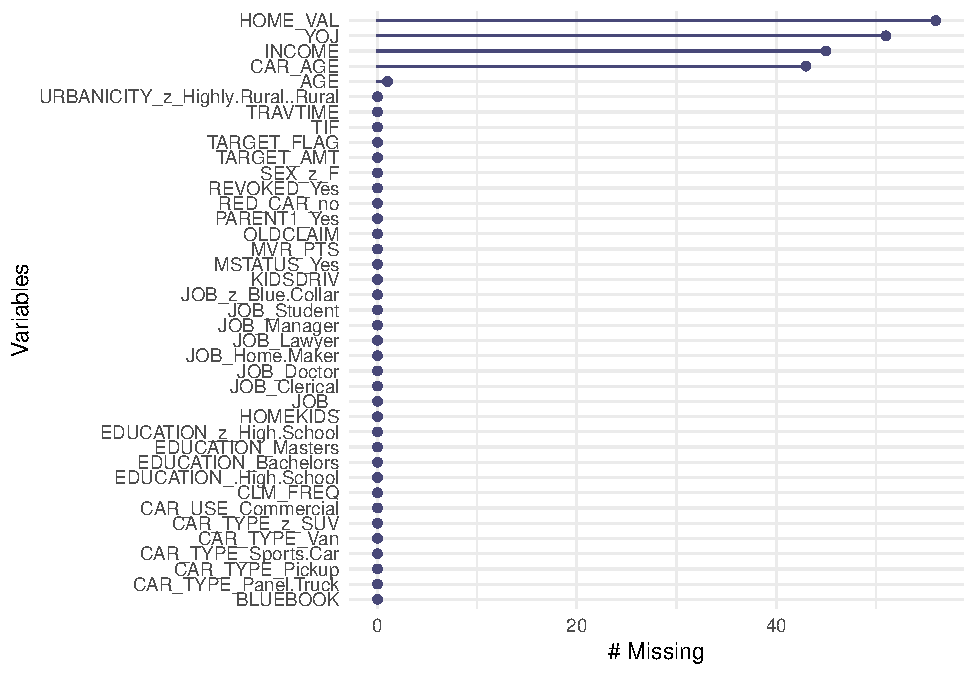
\includegraphics{Baseball5_files/figure-latex/unnamed-chunk-7-1.pdf}

\begin{Shaded}
\begin{Highlighting}[]
\FunctionTok{grid.arrange}\NormalTok{(}\AttributeTok{grobs=}\NormalTok{z1[}\FunctionTok{c}\NormalTok{(}\DecValTok{8}\SpecialCharTok{:}\DecValTok{13}\NormalTok{)],  }\AttributeTok{ncol=}\DecValTok{2}\NormalTok{, }\AttributeTok{nrow=}\DecValTok{3}\NormalTok{)}
\end{Highlighting}
\end{Shaded}

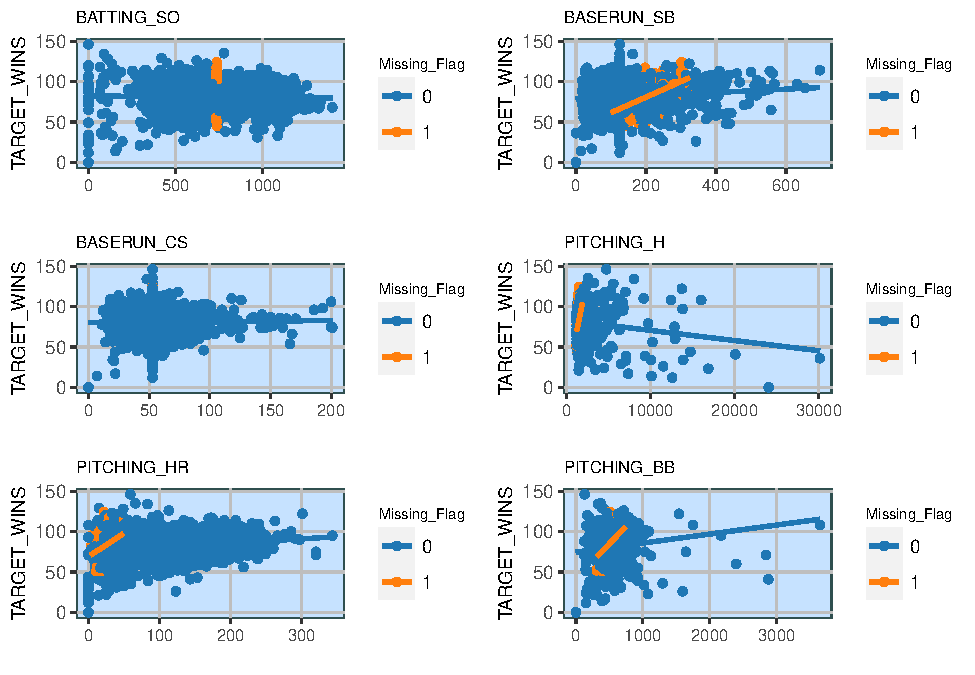
\includegraphics{Baseball5_files/figure-latex/unnamed-chunk-7-2.pdf}

\begin{Shaded}
\begin{Highlighting}[]
\FunctionTok{grid.arrange}\NormalTok{(}\AttributeTok{grobs=}\NormalTok{z1[}\FunctionTok{c}\NormalTok{(}\DecValTok{14}\SpecialCharTok{:}\DecValTok{16}\NormalTok{)],  }\AttributeTok{ncol=}\DecValTok{2}\NormalTok{, }\AttributeTok{nrow=}\DecValTok{3}\NormalTok{)}
\end{Highlighting}
\end{Shaded}

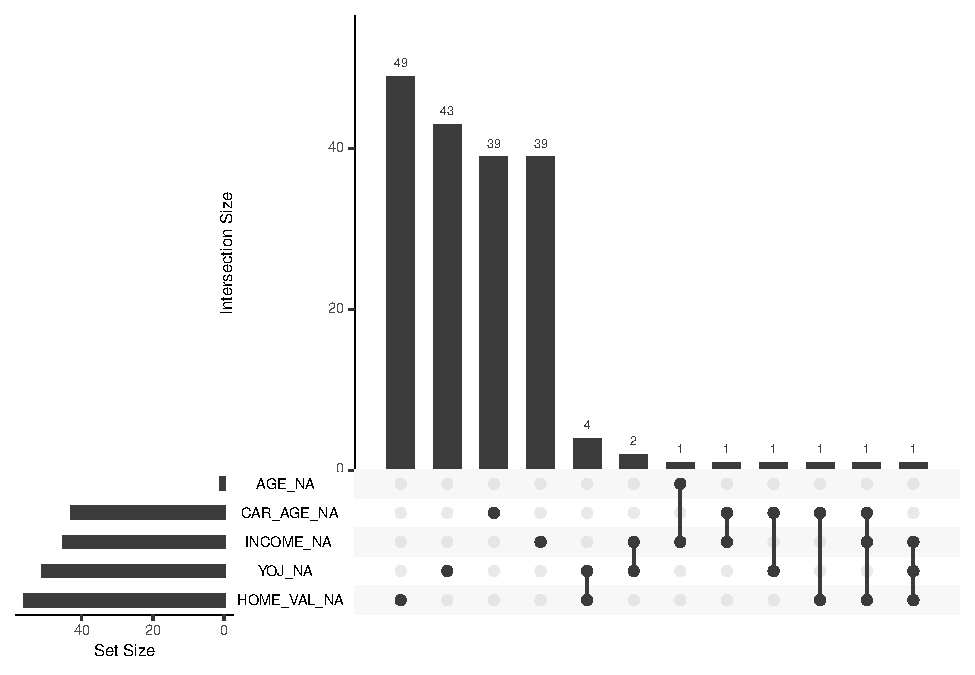
\includegraphics{Baseball5_files/figure-latex/unnamed-chunk-7-3.pdf}

The interaction analysis suggests that the cohort is not random - there
are numerous interactions with many other variables, some of which are
quite counterinutitive (team pitching H). So we could either do a random
effects/flag/interactions or toss them. Becuase bad data is not
reproducible I will toss, at the expense of better predicitons if I can
identify the cohort in the eval data.

No we can look at the stats in ur new dataset.

\begin{Shaded}
\begin{Highlighting}[]
\FunctionTok{summary}\NormalTok{(dfTrain\_ImputedMean\_NoCohort)}
\end{Highlighting}
\end{Shaded}

\begin{verbatim}
##      INDEX         TARGET_WINS       BATTING_H      BATTING_2B   
##  Min.   :   1.0   Min.   :  0.00   Min.   : 891   Min.   : 69.0  
##  1st Qu.: 640.2   1st Qu.: 71.00   1st Qu.:1389   1st Qu.:211.2  
##  Median :1275.5   Median : 82.00   Median :1458   Median :240.0  
##  Mean   :1275.2   Mean   : 80.76   Mean   :1475   Mean   :243.9  
##  3rd Qu.:1923.8   3rd Qu.: 91.00   3rd Qu.:1541   3rd Qu.:275.0  
##  Max.   :2535.0   Max.   :146.00   Max.   :2554   Max.   :458.0  
##    BATTING_3B       BATTING_HR      BATTING_BB      BATTING_SO    
##  Min.   :  0.00   Min.   :  0.0   Min.   :  0.0   Min.   :   0.0  
##  1st Qu.: 34.00   1st Qu.: 48.0   1st Qu.:456.0   1st Qu.: 548.0  
##  Median : 46.00   Median :107.0   Median :517.0   Median : 750.0  
##  Mean   : 54.45   Mean   :103.4   Mean   :505.1   Mean   : 735.6  
##  3rd Qu.: 71.00   3rd Qu.:148.0   3rd Qu.:582.0   3rd Qu.: 930.0  
##  Max.   :223.00   Max.   :264.0   Max.   :878.0   Max.   :1399.0  
##    BASERUN_SB      BASERUN_CS      PITCHING_H     PITCHING_HR   
##  Min.   :  0.0   Min.   :  0.0   Min.   : 1137   Min.   :  0.0  
##  1st Qu.: 66.0   1st Qu.: 44.0   1st Qu.: 1425   1st Qu.: 58.0  
##  Median :102.0   Median : 52.8   Median : 1521   Median :111.0  
##  Mean   :121.1   Mean   : 52.8   Mean   : 1794   Mean   :109.7  
##  3rd Qu.:143.8   3rd Qu.: 55.0   3rd Qu.: 1694   3rd Qu.:152.8  
##  Max.   :697.0   Max.   :201.0   Max.   :30132   Max.   :343.0  
##   PITCHING_BB      PITCHING_SO        FIELDING_E      FIELDING_DP   
##  Min.   :   0.0   Min.   :    0.0   Min.   :  65.0   Min.   : 52.0  
##  1st Qu.: 479.2   1st Qu.:  615.0   1st Qu.: 126.0   1st Qu.:137.0  
##  Median : 542.0   Median :  813.5   Median : 155.0   Median :146.4  
##  Mean   : 557.5   Mean   :  817.7   Mean   : 243.9   Mean   :148.6  
##  3rd Qu.: 614.8   3rd Qu.:  968.0   3rd Qu.: 234.0   3rd Qu.:162.0  
##  Max.   :3645.0   Max.   :19278.0   Max.   :1898.0   Max.   :228.0
\end{verbatim}

\hypertarget{now-we-can-do-outlier-analysis-and-check-to-see-if-zeroes-may-be-coded-as-nas}{%
\subsubsection{Now we can do Outlier Analysis, and check to see if
zeroes may be coded as
nas}\label{now-we-can-do-outlier-analysis-and-check-to-see-if-zeroes-may-be-coded-as-nas}}

\begin{Shaded}
\begin{Highlighting}[]
\NormalTok{EHExplore\_Outliers\_Boxplots }\OtherTok{\textless{}{-}} \ControlFlowTok{function}\NormalTok{(df, }\AttributeTok{size=}\StringTok{"small"}\NormalTok{)}
\NormalTok{\{}

\NormalTok{df }\OtherTok{\textless{}{-}} \FunctionTok{select\_if}\NormalTok{(df, is.numeric)}
  
\NormalTok{s }\OtherTok{\textless{}{-}} \DecValTok{7}
\ControlFlowTok{if}\NormalTok{ (size}\SpecialCharTok{==}\StringTok{"large"}\NormalTok{) \{}
\NormalTok{  s }\OtherTok{\textless{}{-}} \DecValTok{10}
\NormalTok{\}}
\NormalTok{plot\_list2 }\OtherTok{\textless{}{-}} \FunctionTok{list}\NormalTok{()}

\ControlFlowTok{for}\NormalTok{(i }\ControlFlowTok{in} \DecValTok{1}\SpecialCharTok{:}\FunctionTok{ncol}\NormalTok{(df)) \{     }
  
\NormalTok{  qp }\OtherTok{\textless{}{-}} \FunctionTok{toString}\NormalTok{(}\FunctionTok{head}\NormalTok{(}\FunctionTok{sort}\NormalTok{(}\FunctionTok{round}\NormalTok{(df[,i],}\DecValTok{2}\NormalTok{)),}\DecValTok{5}\NormalTok{))}
\NormalTok{  qz }\OtherTok{\textless{}{-}} \FunctionTok{toString}\NormalTok{(}\FunctionTok{tail}\NormalTok{(}\FunctionTok{sort}\NormalTok{(}\FunctionTok{round}\NormalTok{(df[,i],}\DecValTok{2}\NormalTok{)),}\DecValTok{5}\NormalTok{))}
\NormalTok{  qk }\OtherTok{\textless{}{-}} \FunctionTok{str\_c}\NormalTok{(}\StringTok{"L:   "}\NormalTok{, qp, }\StringTok{"}\SpecialCharTok{\textbackslash{}\textbackslash{}\textbackslash{}n}\StringTok{"}\NormalTok{, }\StringTok{"H:   "}\NormalTok{, qz)}
  
\NormalTok{  p }\OtherTok{\textless{}{-}} \FunctionTok{eval}\NormalTok{(}\FunctionTok{substitute}\NormalTok{(}\FunctionTok{ggplot}\NormalTok{(df, }\FunctionTok{aes}\NormalTok{(df[,i])) }\SpecialCharTok{+}
          \FunctionTok{coord\_flip}\NormalTok{() }\SpecialCharTok{+}  
          \FunctionTok{xlab}\NormalTok{(}\FunctionTok{colnames}\NormalTok{(df)[i])  }\SpecialCharTok{+}
          \FunctionTok{ylab}\NormalTok{(qk) }\SpecialCharTok{+}
          \FunctionTok{theme}\NormalTok{(}\AttributeTok{axis.title.x =} \FunctionTok{element\_text}\NormalTok{(}\AttributeTok{size =}\NormalTok{ s), }\AttributeTok{axis.title.y =} \FunctionTok{element\_text}\NormalTok{(}\AttributeTok{size =} \DecValTok{9}\NormalTok{), }\AttributeTok{axis.text.x =} \FunctionTok{element\_blank}\NormalTok{(), }\AttributeTok{axis.ticks.x =} \FunctionTok{element\_blank}\NormalTok{(), }\AttributeTok{panel.grid.major.x =} \FunctionTok{element\_blank}\NormalTok{(), }\AttributeTok{panel.grid.minor.x=}\FunctionTok{element\_blank}\NormalTok{(), }\AttributeTok{panel.grid.minor.y=}\FunctionTok{element\_blank}\NormalTok{(), }\AttributeTok{panel.grid.major.y=}\FunctionTok{element\_line}\NormalTok{(}\AttributeTok{color=}\StringTok{"gray"}\NormalTok{), }\AttributeTok{panel.background =} \FunctionTok{element\_rect}\NormalTok{(}\AttributeTok{fill =} \StringTok{"slategray2"}\NormalTok{, }\AttributeTok{color=}\StringTok{"darkslategray"}\NormalTok{))  }\SpecialCharTok{+} 
          \FunctionTok{geom\_boxplot}\NormalTok{(), }\FunctionTok{list}\NormalTok{(}\AttributeTok{i=}\NormalTok{i)))}
\NormalTok{  plot\_list2[[i]] }\OtherTok{\textless{}{-}}\NormalTok{ p }
  
  
\NormalTok{\}}
\FunctionTok{return}\NormalTok{ (plot\_list2)}
\NormalTok{\}}


\NormalTok{z }\OtherTok{\textless{}{-}} \FunctionTok{EHExplore\_Outliers\_Boxplots}\NormalTok{(dfTrain\_ImputedMean\_NoCohort, }\StringTok{"small"}\NormalTok{)}
\FunctionTok{wrap\_plots}\NormalTok{(z)}
\end{Highlighting}
\end{Shaded}

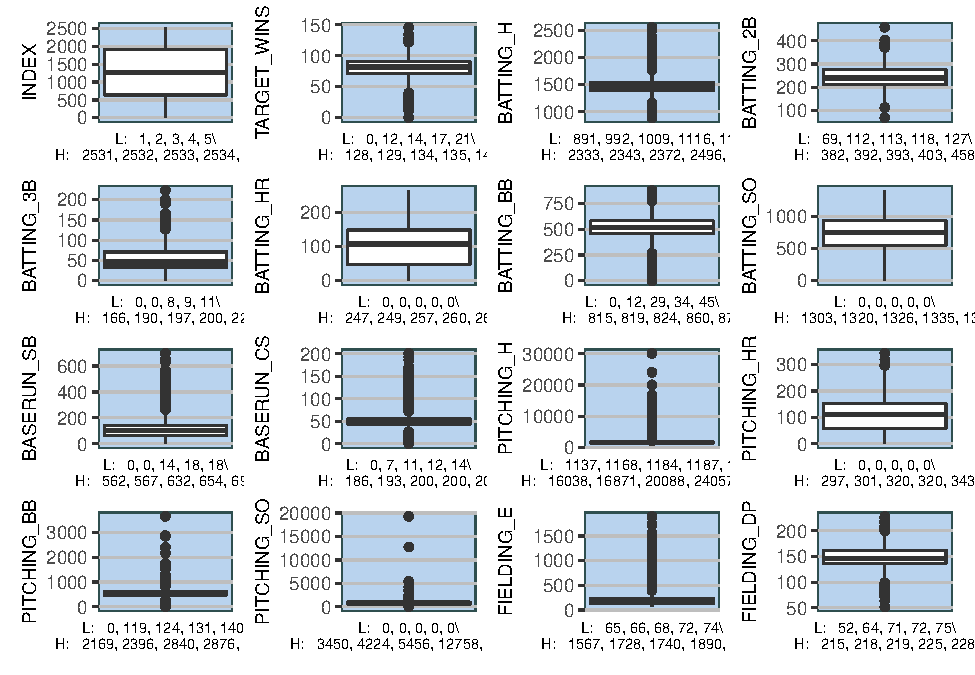
\includegraphics{Baseball5_files/figure-latex/unnamed-chunk-9-1.pdf}

\begin{Shaded}
\begin{Highlighting}[]
\NormalTok{EHExplore\_Distributions\_Histograms }\OtherTok{\textless{}{-}} \ControlFlowTok{function}\NormalTok{(df, }\AttributeTok{size =} \StringTok{"small"}\NormalTok{, }\AttributeTok{nbins =} \DecValTok{100}\NormalTok{)}
\NormalTok{\{}
  
\NormalTok{df }\OtherTok{\textless{}{-}} \FunctionTok{select\_if}\NormalTok{(df, is.numeric)}
    
\NormalTok{s }\OtherTok{\textless{}{-}} \DecValTok{7}
\ControlFlowTok{if}\NormalTok{ (size}\SpecialCharTok{==}\StringTok{"large"}\NormalTok{) \{}
\NormalTok{  s }\OtherTok{\textless{}{-}} \DecValTok{10}
\NormalTok{\}}

\NormalTok{plot\_list2 }\OtherTok{\textless{}{-}} \FunctionTok{list}\NormalTok{()}

\ControlFlowTok{for}\NormalTok{(i }\ControlFlowTok{in} \DecValTok{1}\SpecialCharTok{:}\FunctionTok{ncol}\NormalTok{(df)) \{     }
  
\NormalTok{  qp }\OtherTok{\textless{}{-}} \FunctionTok{toString}\NormalTok{(}\FunctionTok{head}\NormalTok{(}\FunctionTok{sort}\NormalTok{(}\FunctionTok{round}\NormalTok{(df[,i],}\DecValTok{2}\NormalTok{)),}\DecValTok{5}\NormalTok{))}
\NormalTok{  qz }\OtherTok{\textless{}{-}} \FunctionTok{toString}\NormalTok{(}\FunctionTok{tail}\NormalTok{(}\FunctionTok{sort}\NormalTok{(}\FunctionTok{round}\NormalTok{(df[,i],}\DecValTok{2}\NormalTok{)),}\DecValTok{5}\NormalTok{))}
\NormalTok{  qk }\OtherTok{\textless{}{-}} \FunctionTok{str\_c}\NormalTok{(}\StringTok{"L:   "}\NormalTok{, qp, }\StringTok{"}\SpecialCharTok{\textbackslash{}\textbackslash{}\textbackslash{}n}\StringTok{"}\NormalTok{, }\StringTok{"H:   "}\NormalTok{, qz)}
  
\NormalTok{  p }\OtherTok{\textless{}{-}} \FunctionTok{eval}\NormalTok{(}\FunctionTok{substitute}\NormalTok{(}\FunctionTok{ggplot}\NormalTok{(df, }\FunctionTok{aes}\NormalTok{(df[,i])) }\SpecialCharTok{+}
          \FunctionTok{ylab}\NormalTok{(}\FunctionTok{colnames}\NormalTok{(df)[i])  }\SpecialCharTok{+}
          \FunctionTok{xlab}\NormalTok{(qk) }\SpecialCharTok{+}
          \FunctionTok{theme}\NormalTok{(}\AttributeTok{axis.title.x =} \FunctionTok{element\_text}\NormalTok{(}\AttributeTok{size =}\NormalTok{ s), }\AttributeTok{axis.title.y =} \FunctionTok{element\_text}\NormalTok{(}\AttributeTok{size =} \DecValTok{9}\NormalTok{), }\AttributeTok{axis.text.y =} \FunctionTok{element\_blank}\NormalTok{(), }\AttributeTok{axis.ticks.y =} \FunctionTok{element\_blank}\NormalTok{(), }\AttributeTok{axis.text.x =} \FunctionTok{element\_text}\NormalTok{(}\AttributeTok{size=}\DecValTok{8}\NormalTok{),  }\AttributeTok{panel.grid.major.x =} \FunctionTok{element\_blank}\NormalTok{(), }\AttributeTok{panel.grid.minor.x=}\FunctionTok{element\_blank}\NormalTok{(), }\AttributeTok{panel.grid.minor.y=}\FunctionTok{element\_blank}\NormalTok{(), }\AttributeTok{panel.grid.major.y=}\FunctionTok{element\_blank}\NormalTok{(), }\AttributeTok{panel.background =} \FunctionTok{element\_rect}\NormalTok{(}\AttributeTok{fill =} \StringTok{"slategray2"}\NormalTok{, }\AttributeTok{color=}\StringTok{"darkslategray"}\NormalTok{))  }\SpecialCharTok{+} 
  \FunctionTok{geom\_histogram}\NormalTok{(}\AttributeTok{bins=}\NormalTok{nbins, }\AttributeTok{fill=}\StringTok{"white"}\NormalTok{, }\FunctionTok{aes}\NormalTok{(}\AttributeTok{y =} \FunctionTok{stat}\NormalTok{(density))) }\SpecialCharTok{+}
      \FunctionTok{geom\_density}\NormalTok{(}\AttributeTok{col =} \StringTok{"red"}\NormalTok{), }\FunctionTok{list}\NormalTok{(}\AttributeTok{i=}\NormalTok{i)))}
\NormalTok{  plot\_list2[[i]] }\OtherTok{\textless{}{-}}\NormalTok{ p }
  
\NormalTok{\}}
\FunctionTok{return}\NormalTok{ (plot\_list2)}
\NormalTok{\}}

\NormalTok{z6 }\OtherTok{\textless{}{-}} \FunctionTok{EHExplore\_Distributions\_Histograms}\NormalTok{(dfTrain\_ImputedMean\_NoCohort, }\StringTok{"small"}\NormalTok{)}
\FunctionTok{wrap\_plots}\NormalTok{(z6)}
\end{Highlighting}
\end{Shaded}

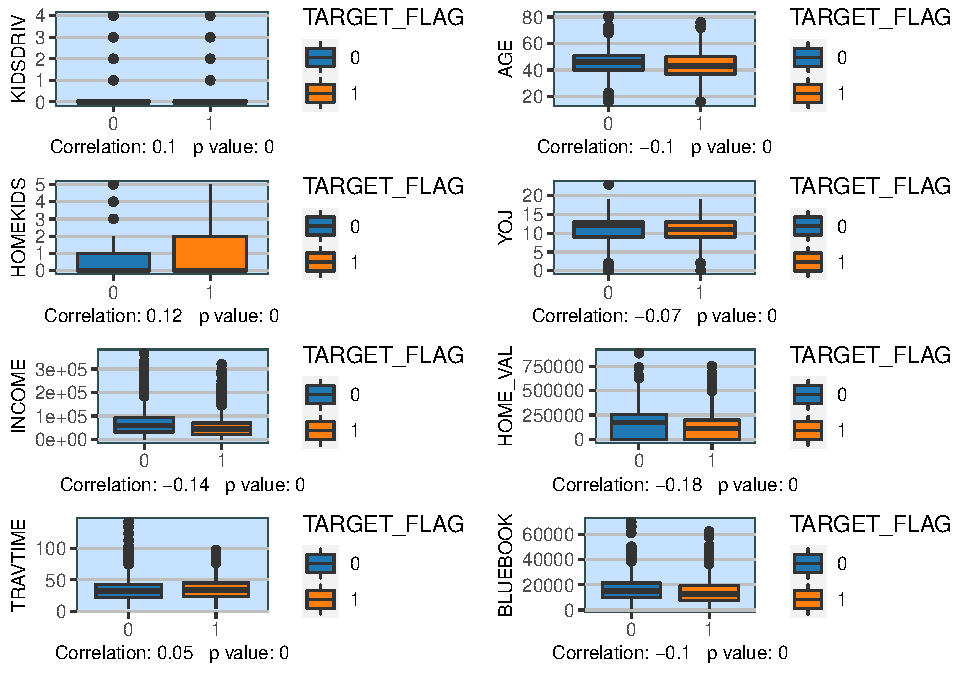
\includegraphics{Baseball5_files/figure-latex/unnamed-chunk-10-1.pdf}

\begin{Shaded}
\begin{Highlighting}[]
\CommentTok{\#zz1 \textless{}{-} EHExplore\_CombineGraphs(z, z4, z6)}

\CommentTok{\#grid.arrange(grobs=zz1[c(1:16)],  ncol=4, nrow=4)}
\CommentTok{\#grid.arrange(grobs=zz1[c(17:32)],  ncol=4, nrow=4)}
\end{Highlighting}
\end{Shaded}

There are 4 categories where 0s may be nas: Pitching and Batting HR and
Pitching and batting SO. We look more closely at these categories:

\begin{Shaded}
\begin{Highlighting}[]
\NormalTok{dfTrain\_ZeroAsNA }\OtherTok{\textless{}{-}}\NormalTok{ dfTrain }\SpecialCharTok{\%\textgreater{}\%}
\NormalTok{dplyr}\SpecialCharTok{::}\FunctionTok{select}\NormalTok{(PITCHING\_SO, PITCHING\_HR, BATTING\_SO, BATTING\_HR)}

\FunctionTok{hist}\NormalTok{(dfTrain\_ZeroAsNA)}
\end{Highlighting}
\end{Shaded}

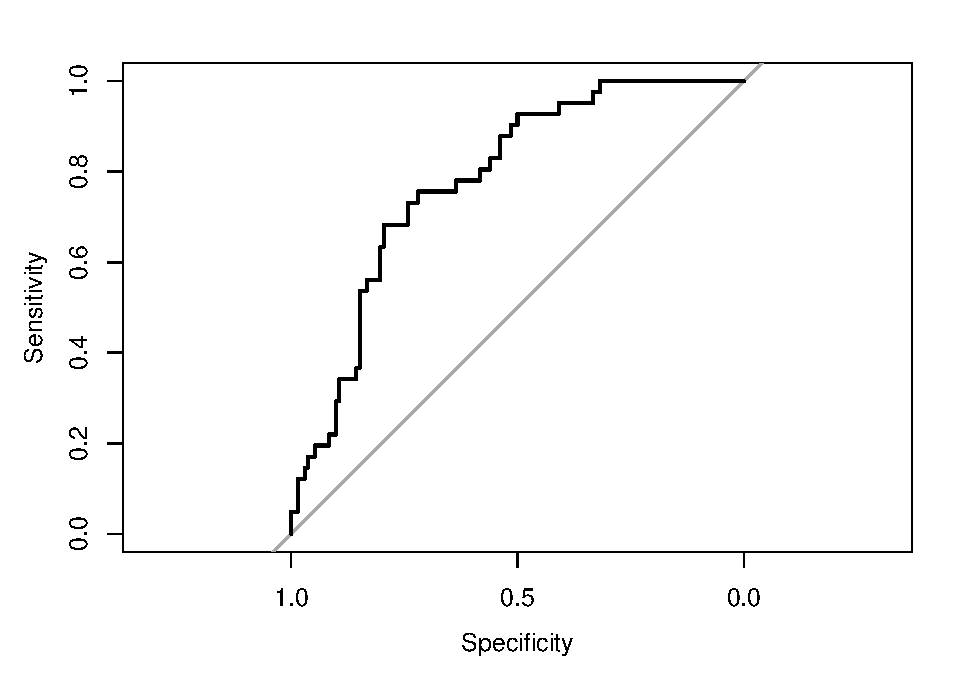
\includegraphics{Baseball5_files/figure-latex/unnamed-chunk-12-1.pdf}

We can check to see if the zeroes behave like nas or actual values. We
compare the interaction with Pitching\_h in both cases. They behave very
differently, neither like the overall sample:

\begin{Shaded}
\begin{Highlighting}[]
\NormalTok{dfTmp }\OtherTok{\textless{}{-}}\NormalTok{ dfTrain\_ImputedMean }\SpecialCharTok{\%\textgreater{}\%}
  \FunctionTok{mutate}\NormalTok{(}\AttributeTok{Zeros =} \FunctionTok{ifelse}\NormalTok{(PITCHING\_SO }\SpecialCharTok{\textless{}=} \DecValTok{0}\NormalTok{, }\DecValTok{1}\NormalTok{, }\DecValTok{0}\NormalTok{))}

\NormalTok{z2 }\OtherTok{\textless{}{-}} \FunctionTok{EHExplore\_Interactions\_Scatterplots}\NormalTok{(dfTmp, }\StringTok{"TARGET\_WINS"}\NormalTok{, }\StringTok{"Zeros"}\NormalTok{)}

\FunctionTok{grid.arrange}\NormalTok{(z2[[}\DecValTok{11}\NormalTok{]], z1[[}\DecValTok{11}\NormalTok{]],  }\AttributeTok{ncol=}\DecValTok{2}\NormalTok{, }\AttributeTok{nrow=}\DecValTok{3}\NormalTok{)}
\end{Highlighting}
\end{Shaded}

\begin{verbatim}
## `geom_smooth()` using formula 'y ~ x'
## `geom_smooth()` using formula 'y ~ x'
\end{verbatim}

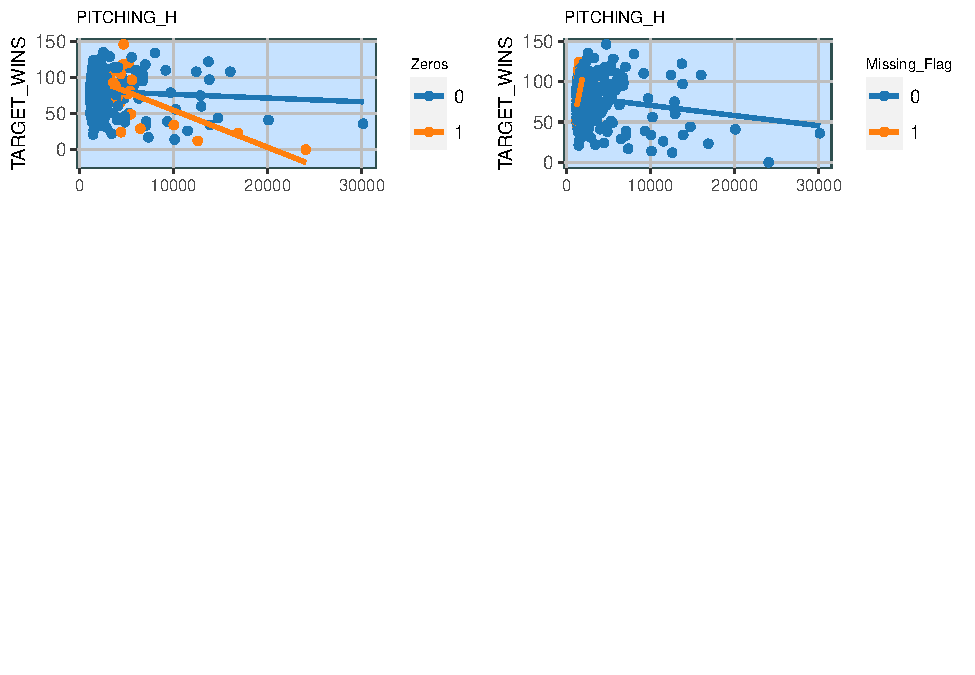
\includegraphics{Baseball5_files/figure-latex/unnamed-chunk-13-1.pdf}
Looking for other gorups, Hard to say - there seems to be something
about lower so being more negatively correlated with wins than later -
but the ns may be small:

\begin{Shaded}
\begin{Highlighting}[]
\NormalTok{dfTmp }\OtherTok{\textless{}{-}}\NormalTok{ dfTrain\_ImputedMean }\SpecialCharTok{\%\textgreater{}\%}
  \FunctionTok{mutate}\NormalTok{(}\AttributeTok{Zeros =} \FunctionTok{ifelse}\NormalTok{(PITCHING\_SO }\SpecialCharTok{\textless{}=} \DecValTok{400} \SpecialCharTok{\&}\NormalTok{ PITCHING\_SO }\SpecialCharTok{\textgreater{}=}\DecValTok{0}\NormalTok{, }\DecValTok{1}\NormalTok{, }\DecValTok{0}\NormalTok{))}

\NormalTok{dfx }\OtherTok{\textless{}{-}}\NormalTok{ dfTmp }\SpecialCharTok{\%\textgreater{}\%}
  \FunctionTok{filter}\NormalTok{(Zeros}\SpecialCharTok{==}\DecValTok{1}\NormalTok{)}

\NormalTok{z2 }\OtherTok{\textless{}{-}} \FunctionTok{EHExplore\_Interactions\_Scatterplots}\NormalTok{(dfTmp, }\StringTok{"TARGET\_WINS"}\NormalTok{, }\StringTok{"Zeros"}\NormalTok{)}

\FunctionTok{grid.arrange}\NormalTok{(z2[[}\DecValTok{11}\NormalTok{]], z1[[}\DecValTok{11}\NormalTok{]],  }\AttributeTok{ncol=}\DecValTok{2}\NormalTok{, }\AttributeTok{nrow=}\DecValTok{3}\NormalTok{)}
\end{Highlighting}
\end{Shaded}

\begin{verbatim}
## `geom_smooth()` using formula 'y ~ x'
## `geom_smooth()` using formula 'y ~ x'
\end{verbatim}

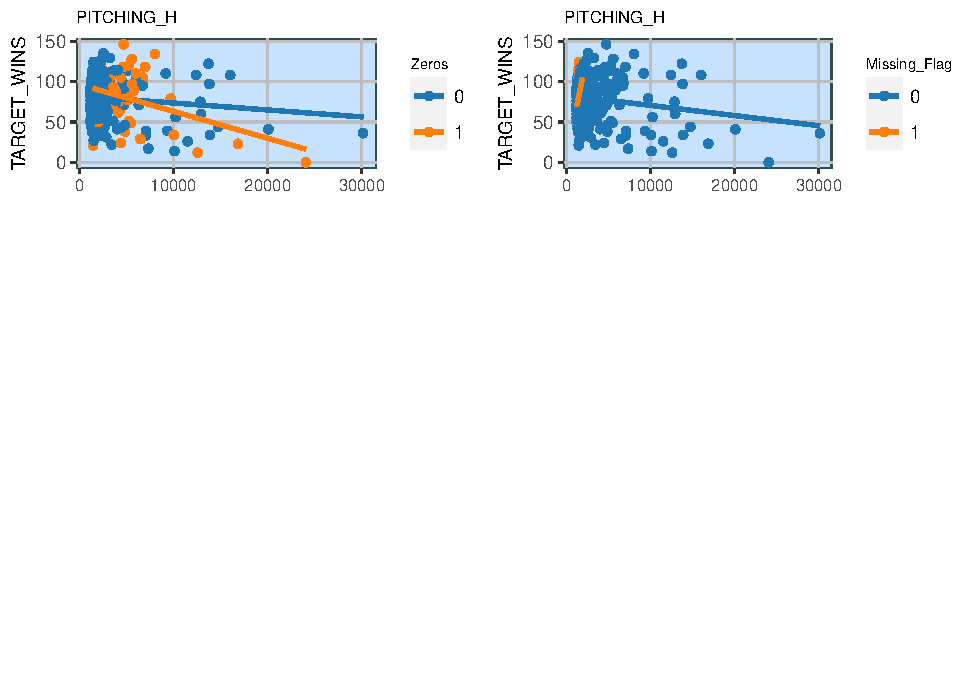
\includegraphics{Baseball5_files/figure-latex/unnamed-chunk-14-1.pdf}

Will do nothing with outliers or na as zero for now

\hypertarget{second-exploration}{%
\subsubsection{Second Exploration}\label{second-exploration}}

\hypertarget{a.-dependent-variable}{%
\paragraph{a. Dependent variable}\label{a.-dependent-variable}}

\begin{Shaded}
\begin{Highlighting}[]
\FunctionTok{hist}\NormalTok{(dfTrain}\SpecialCharTok{$}\NormalTok{TARGET\_WINS, }\AttributeTok{bins=}\DecValTok{20}\NormalTok{)}
\end{Highlighting}
\end{Shaded}

\begin{verbatim}
## Warning in plot.window(xlim, ylim, "", ...): "bins" is not a graphical parameter
\end{verbatim}

\begin{verbatim}
## Warning in title(main = main, sub = sub, xlab = xlab, ylab = ylab, ...): "bins"
## is not a graphical parameter
\end{verbatim}

\begin{verbatim}
## Warning in axis(1, ...): "bins" is not a graphical parameter
\end{verbatim}

\begin{verbatim}
## Warning in axis(2, ...): "bins" is not a graphical parameter
\end{verbatim}

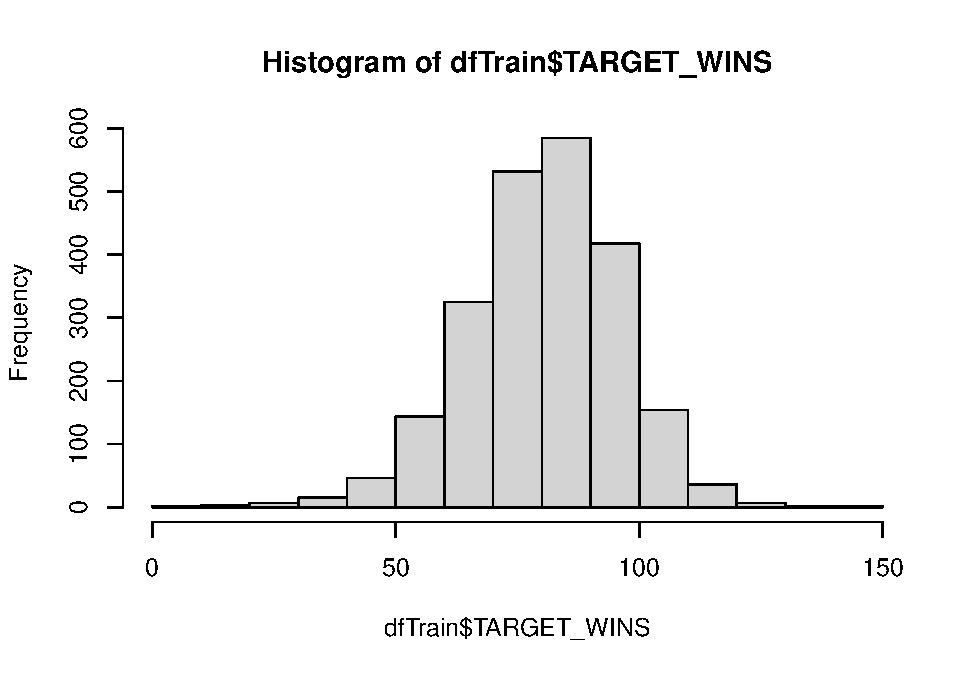
\includegraphics{Baseball5_files/figure-latex/unnamed-chunk-15-1.pdf}

\begin{Shaded}
\begin{Highlighting}[]
\FunctionTok{head}\NormalTok{(}\FunctionTok{sort}\NormalTok{(dfTrain}\SpecialCharTok{$}\NormalTok{TARGET\_WINS))}
\end{Highlighting}
\end{Shaded}

\begin{verbatim}
## [1]  0 12 14 17 21 22
\end{verbatim}

\begin{Shaded}
\begin{Highlighting}[]
\NormalTok{dfTrain\_ZeroWins }\OtherTok{\textless{}{-}}\NormalTok{ dfTrain }\SpecialCharTok{\%\textgreater{}\%}
\NormalTok{  dplyr}\SpecialCharTok{::}\FunctionTok{filter}\NormalTok{(TARGET\_WINS }\SpecialCharTok{==}\DecValTok{0}\NormalTok{)}

\FunctionTok{head}\NormalTok{(dfTrain\_ZeroWins, }\DecValTok{1}\NormalTok{)}
\end{Highlighting}
\end{Shaded}

\begin{verbatim}
##   INDEX TARGET_WINS BATTING_H BATTING_2B BATTING_3B BATTING_HR BATTING_BB
## 1  1347           0       891        135          0          0          0
##   BATTING_SO BASERUN_SB BASERUN_CS BATTING_HBP PITCHING_H PITCHING_HR
## 1          0          0          0          NA      24057           0
##   PITCHING_BB PITCHING_SO FIELDING_E FIELDING_DP
## 1           0           0       1890          NA
\end{verbatim}

Target\_Wins appears normally distributed - the zero is suspicious but
I'm going to leave it.

\hypertarget{b.-look-at-correlations-throughout-the-variables-and-inspect-multi-colinnearity}{%
\paragraph{b. Look at correlations throughout the variables and inspect
multi-colinnearity}\label{b.-look-at-correlations-throughout-the-variables-and-inspect-multi-colinnearity}}

\begin{Shaded}
\begin{Highlighting}[]
\NormalTok{dfCor }\OtherTok{\textless{}{-}} \FunctionTok{as.data.frame}\NormalTok{(}\FunctionTok{cor}\NormalTok{(dfTrain\_ImputedMean\_NoCohort))}
\NormalTok{dfCor}
\end{Highlighting}
\end{Shaded}

\begin{verbatim}
##                     INDEX TARGET_WINS   BATTING_H   BATTING_2B  BATTING_3B
## INDEX        1.0000000000 -0.02928140 -0.03131390 -0.003976934 -0.00497585
## TARGET_WINS -0.0292813985  1.00000000  0.39476995  0.293205037  0.13685882
## BATTING_H   -0.0313139014  0.39476995  1.00000000  0.540648272  0.45802046
## BATTING_2B  -0.0039769341  0.29320504  0.54064827  1.000000000 -0.08532550
## BATTING_3B  -0.0049758496  0.13685882  0.45802046 -0.085325497  1.00000000
## BATTING_HR   0.0413809930  0.19059035 -0.06194956  0.393641975 -0.63765753
## BATTING_BB  -0.0358540809  0.23250609 -0.10545406  0.230196649 -0.28160593
## BATTING_SO   0.0814501106 -0.03175071 -0.46385357  0.162685188 -0.66978119
## BASERUN_SB   0.0435154747  0.11143414  0.14886129 -0.153728585  0.49301668
## BASERUN_CS   0.0004632733  0.01610843  0.01198251 -0.077632602  0.19833581
## PITCHING_H   0.0146890757 -0.11576530  0.29979491  0.008872511  0.20396690
## PITCHING_HR  0.0403725584  0.20531868  0.02082589  0.412455481 -0.56629509
## PITCHING_BB -0.0233549401  0.12063924  0.07067846  0.149565361  0.01294580
## PITCHING_SO  0.0558901457 -0.07843609 -0.25265679  0.064792315 -0.25881893
## FIELDING_E  -0.0068738726 -0.17639551  0.28252119 -0.232247607  0.51354615
## FIELDING_DP  0.0061318975 -0.02860414  0.04535652  0.178563220 -0.21908499
##              BATTING_HR  BATTING_BB  BATTING_SO  BASERUN_SB    BASERUN_CS
## INDEX        0.04138099 -0.03585408  0.08145011  0.04351547  0.0004632733
## TARGET_WINS  0.19059035  0.23250609 -0.03175071  0.11143414  0.0161084320
## BATTING_H   -0.06194956 -0.10545406 -0.46385357  0.14886129  0.0119825143
## BATTING_2B   0.39364197  0.23019665  0.16268519 -0.15372858 -0.0776326024
## BATTING_3B  -0.63765753 -0.28160593 -0.66978119  0.49301668  0.1983358054
## BATTING_HR   1.00000000  0.50439692  0.72706935 -0.39942181 -0.3034743273
## BATTING_BB   0.50439692  1.00000000  0.37975087 -0.06545891 -0.0861202523
## BATTING_SO   0.72706935  0.37975087  1.00000000 -0.23837153 -0.1566149092
## BASERUN_SB  -0.39942181 -0.06545891 -0.23837153  1.00000000  0.2869124889
## BASERUN_CS  -0.30347433 -0.08612025 -0.15661491  0.28691249  1.0000000000
## PITCHING_H  -0.27656010 -0.46585690 -0.37568637  0.07198568 -0.0369545996
## PITCHING_HR  0.96659392  0.44681242  0.66717889 -0.36564098 -0.3034478040
## PITCHING_BB  0.10677385  0.47385394  0.03700514  0.14323815 -0.0542531880
## PITCHING_SO  0.18470756 -0.02075682  0.41623330 -0.05615058 -0.0686217842
## FIELDING_E  -0.59891151 -0.66138116 -0.58466444  0.36999309  0.0236201201
## FIELDING_DP  0.33368751  0.32158157  0.14599850 -0.24957358 -0.1563091914
##               PITCHING_H PITCHING_HR PITCHING_BB PITCHING_SO   FIELDING_E
## INDEX        0.014689076  0.04037256 -0.02335494  0.05589015 -0.006873873
## TARGET_WINS -0.115765302  0.20531868  0.12063924 -0.07843609 -0.176395507
## BATTING_H    0.299794910  0.02082589  0.07067846 -0.25265679  0.282521195
## BATTING_2B   0.008872511  0.41245548  0.14956536  0.06479231 -0.232247607
## BATTING_3B   0.203966905 -0.56629509  0.01294580 -0.25881893  0.513546149
## BATTING_HR  -0.276560100  0.96659392  0.10677385  0.18470756 -0.598911507
## BATTING_BB  -0.465856896  0.44681242  0.47385394 -0.02075682 -0.661381160
## BATTING_SO  -0.375686369  0.66717889  0.03700514  0.41623330 -0.584664436
## BASERUN_SB   0.071985680 -0.36564098  0.14323815 -0.05615058  0.369993094
## BASERUN_CS  -0.036954600 -0.30344780 -0.05425319 -0.06862178  0.023620120
## PITCHING_H   1.000000000 -0.16448724  0.31845282  0.26724807  0.672838853
## PITCHING_HR -0.164487236  1.00000000  0.19575531  0.20588053 -0.501758136
## PITCHING_BB  0.318452818  0.19575531  1.00000000  0.48849865 -0.016375919
## PITCHING_SO  0.267248074  0.20588053  0.48849865  1.00000000 -0.023291783
## FIELDING_E   0.672838853 -0.50175814 -0.01637592 -0.02329178  1.000000000
## FIELDING_DP -0.088957308  0.32336753  0.15211734  0.01039232 -0.257897297
##              FIELDING_DP
## INDEX        0.006131897
## TARGET_WINS -0.028604138
## BATTING_H    0.045356517
## BATTING_2B   0.178563220
## BATTING_3B  -0.219084985
## BATTING_HR   0.333687510
## BATTING_BB   0.321581568
## BATTING_SO   0.145998500
## BASERUN_SB  -0.249573580
## BASERUN_CS  -0.156309191
## PITCHING_H  -0.088957308
## PITCHING_HR  0.323367525
## PITCHING_BB  0.152117341
## PITCHING_SO  0.010392318
## FIELDING_E  -0.257897297
## FIELDING_DP  1.000000000
\end{verbatim}

\begin{Shaded}
\begin{Highlighting}[]
\FunctionTok{heatmap}\NormalTok{(}\FunctionTok{as.matrix}\NormalTok{(dfCor), }\AttributeTok{Rowv =} \ConstantTok{NA}\NormalTok{, }\AttributeTok{Colv =} \ConstantTok{NA}\NormalTok{) }
\end{Highlighting}
\end{Shaded}

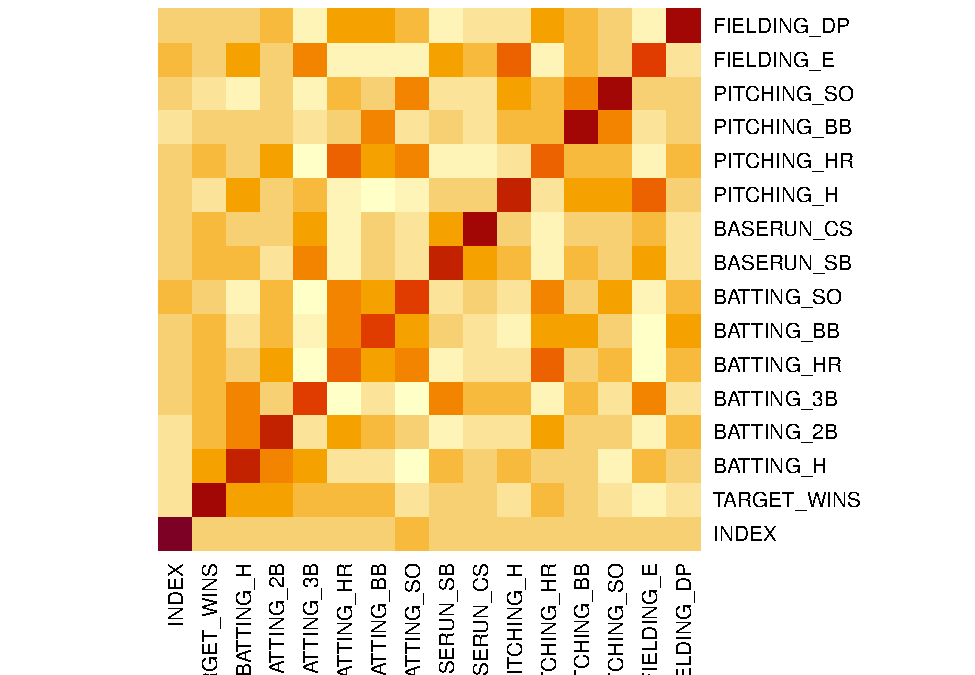
\includegraphics{Baseball5_files/figure-latex/unnamed-chunk-16-1.pdf}

\begin{Shaded}
\begin{Highlighting}[]
\FunctionTok{library}\NormalTok{(corrplot)}
\end{Highlighting}
\end{Shaded}

\begin{verbatim}
## corrplot 0.92 loaded
\end{verbatim}

\begin{Shaded}
\begin{Highlighting}[]
\NormalTok{my\_matrix }\OtherTok{\textless{}{-}}\NormalTok{ dfTrain\_ImputedMean\_NoCohort[]}
\NormalTok{cor\_res }\OtherTok{\textless{}{-}} \FunctionTok{cor}\NormalTok{(my\_matrix, }\AttributeTok{use =} \StringTok{"na.or.complete"}\NormalTok{)}
\FunctionTok{corrplot}\NormalTok{(cor\_res,}
\AttributeTok{type =} \StringTok{"upper"}\NormalTok{,}
\AttributeTok{order =} \StringTok{"original"}\NormalTok{,}
\AttributeTok{tl.col =} \StringTok{"black"}\NormalTok{,}
\AttributeTok{tl.srt =} \DecValTok{45}\NormalTok{,}
\AttributeTok{tl.cex =} \FloatTok{0.55}\NormalTok{)}
\end{Highlighting}
\end{Shaded}

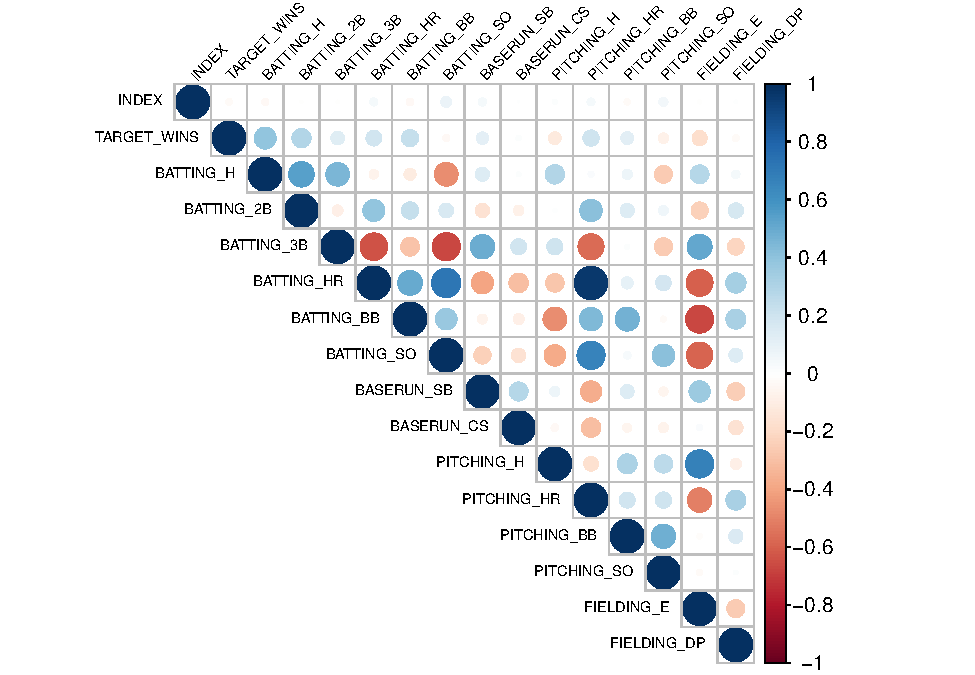
\includegraphics{Baseball5_files/figure-latex/unnamed-chunk-16-2.pdf}

Invsteigate suspicious HR category

\begin{Shaded}
\begin{Highlighting}[]
\FunctionTok{cor.test}\NormalTok{(dfTrain}\SpecialCharTok{$}\NormalTok{PITCHING\_HR, dfTrain}\SpecialCharTok{$}\NormalTok{TARGET\_WINS)}
\end{Highlighting}
\end{Shaded}

\begin{verbatim}
## 
##  Pearson's product-moment correlation
## 
## data:  dfTrain$PITCHING_HR and dfTrain$TARGET_WINS
## t = 9.1789, df = 2274, p-value < 2.2e-16
## alternative hypothesis: true correlation is not equal to 0
## 95 percent confidence interval:
##  0.1490846 0.2283275
## sample estimates:
##       cor 
## 0.1890137
\end{verbatim}

\begin{Shaded}
\begin{Highlighting}[]
\FunctionTok{ggplot}\NormalTok{(dfTrain, }\FunctionTok{aes}\NormalTok{(PITCHING\_HR, BATTING\_HR, }\AttributeTok{color=}\NormalTok{INDEX)) }\SpecialCharTok{+}
  \FunctionTok{geom\_point}\NormalTok{()}
\end{Highlighting}
\end{Shaded}

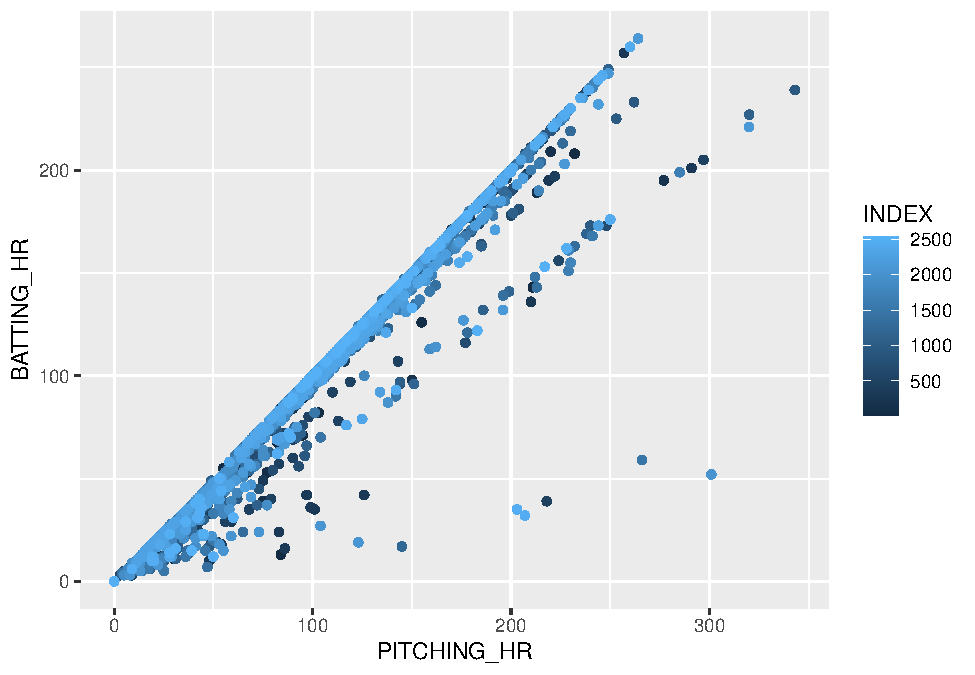
\includegraphics{Baseball5_files/figure-latex/unnamed-chunk-17-1.pdf}

\begin{Shaded}
\begin{Highlighting}[]
\FunctionTok{hist}\NormalTok{(dfTrain}\SpecialCharTok{$}\NormalTok{PITCHING\_HR, }\AttributeTok{breaks=}\DecValTok{100}\NormalTok{)}
\end{Highlighting}
\end{Shaded}

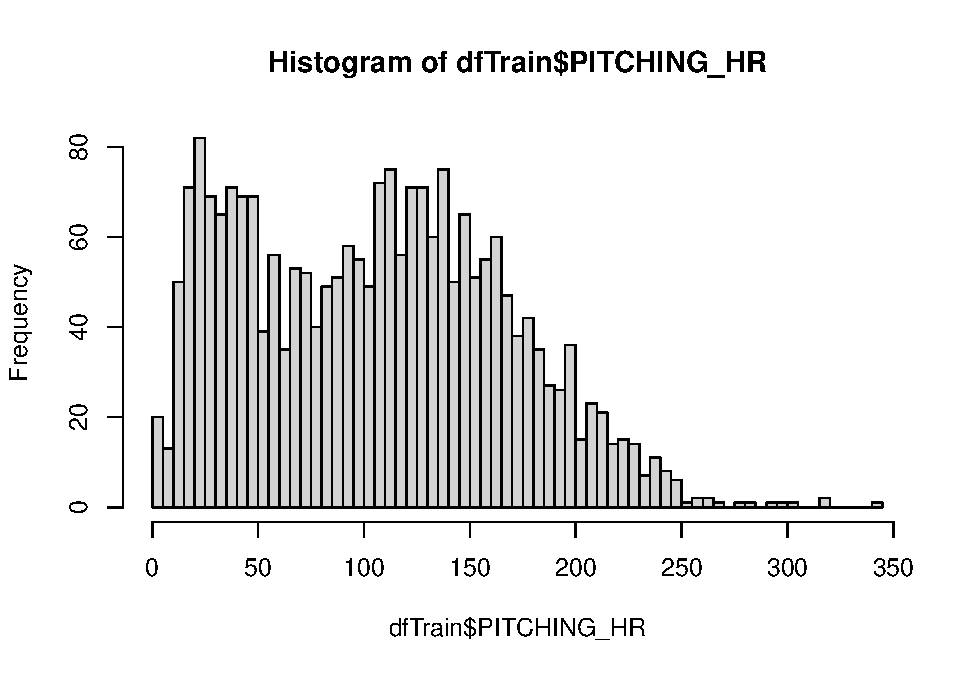
\includegraphics{Baseball5_files/figure-latex/unnamed-chunk-18-1.pdf}

\begin{Shaded}
\begin{Highlighting}[]
\FunctionTok{plot}\NormalTok{(dfTrain}\SpecialCharTok{$}\NormalTok{PITCHING\_HR, dfTrain}\SpecialCharTok{$}\NormalTok{TARGET\_WINS)}
\end{Highlighting}
\end{Shaded}

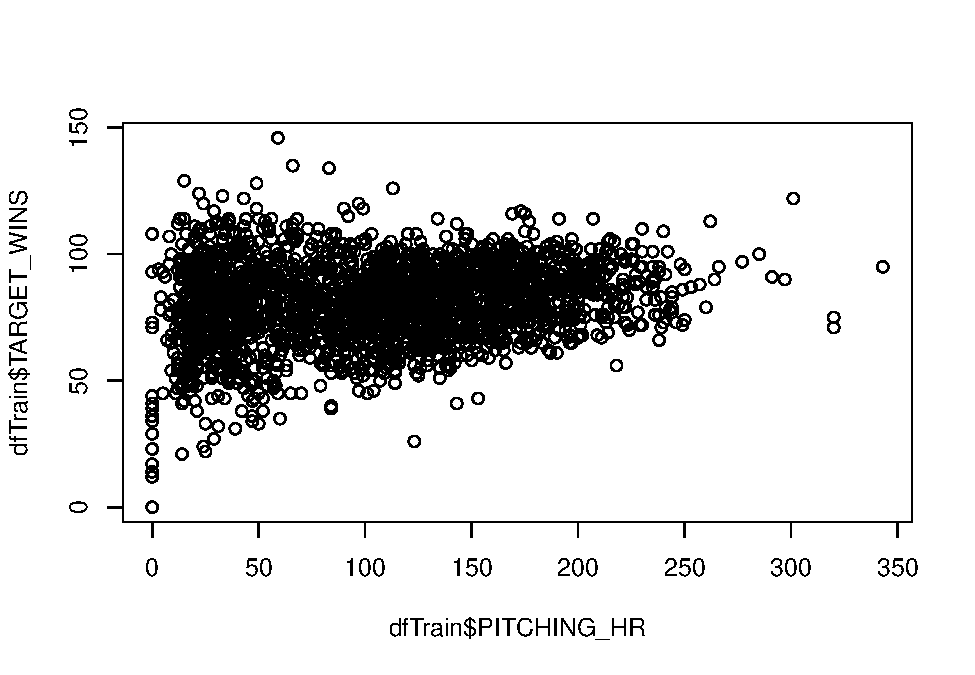
\includegraphics{Baseball5_files/figure-latex/unnamed-chunk-18-2.pdf}

\begin{Shaded}
\begin{Highlighting}[]
\NormalTok{EHModel\_PrintSummary }\OtherTok{\textless{}{-}} \ControlFlowTok{function}\NormalTok{(model)}
\NormalTok{\{}
  \FunctionTok{print}\NormalTok{(}\FunctionTok{summary}\NormalTok{(model))}
  \FunctionTok{par}\NormalTok{(}\AttributeTok{mfcol=}\FunctionTok{c}\NormalTok{(}\DecValTok{2}\NormalTok{,}\DecValTok{2}\NormalTok{))}
  \FunctionTok{print}\NormalTok{(}\FunctionTok{plot}\NormalTok{(model))}
\NormalTok{\}}

\NormalTok{m1 }\OtherTok{\textless{}{-}} \FunctionTok{lm}\NormalTok{(TARGET\_WINS }\SpecialCharTok{\textasciitilde{}}\NormalTok{ PITCHING\_HR, }\AttributeTok{data=}\NormalTok{dfTrain)}
\FunctionTok{summary}\NormalTok{(m1)}
\end{Highlighting}
\end{Shaded}

\begin{verbatim}
## 
## Call:
## lm(formula = TARGET_WINS ~ PITCHING_HR, data = dfTrain)
## 
## Residuals:
##     Min      1Q  Median      3Q     Max 
## -75.657  -9.956   0.636  10.055  67.477 
## 
## Coefficients:
##              Estimate Std. Error t value Pr(>|t|)    
## (Intercept) 75.656920   0.646540 117.018   <2e-16 ***
## PITCHING_HR  0.048572   0.005292   9.179   <2e-16 ***
## ---
## Signif. codes:  0 '***' 0.001 '**' 0.01 '*' 0.05 '.' 0.1 ' ' 1
## 
## Residual standard error: 15.47 on 2274 degrees of freedom
## Multiple R-squared:  0.03573,    Adjusted R-squared:  0.0353 
## F-statistic: 84.25 on 1 and 2274 DF,  p-value: < 2.2e-16
\end{verbatim}

\begin{Shaded}
\begin{Highlighting}[]
\FunctionTok{plot}\NormalTok{(m1)}
\end{Highlighting}
\end{Shaded}

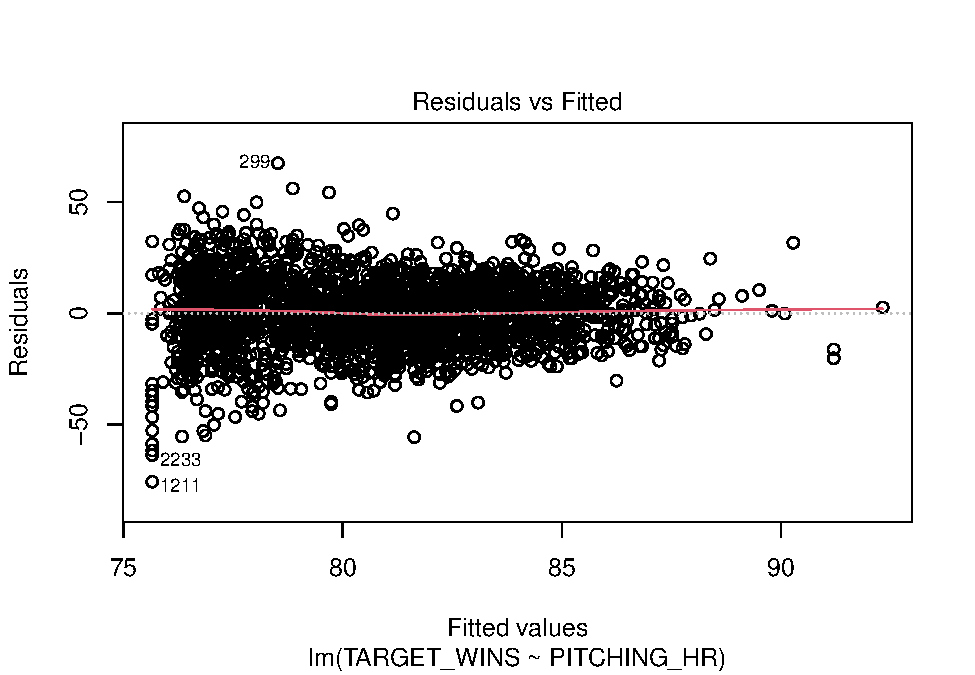
\includegraphics{Baseball5_files/figure-latex/unnamed-chunk-19-1.pdf}
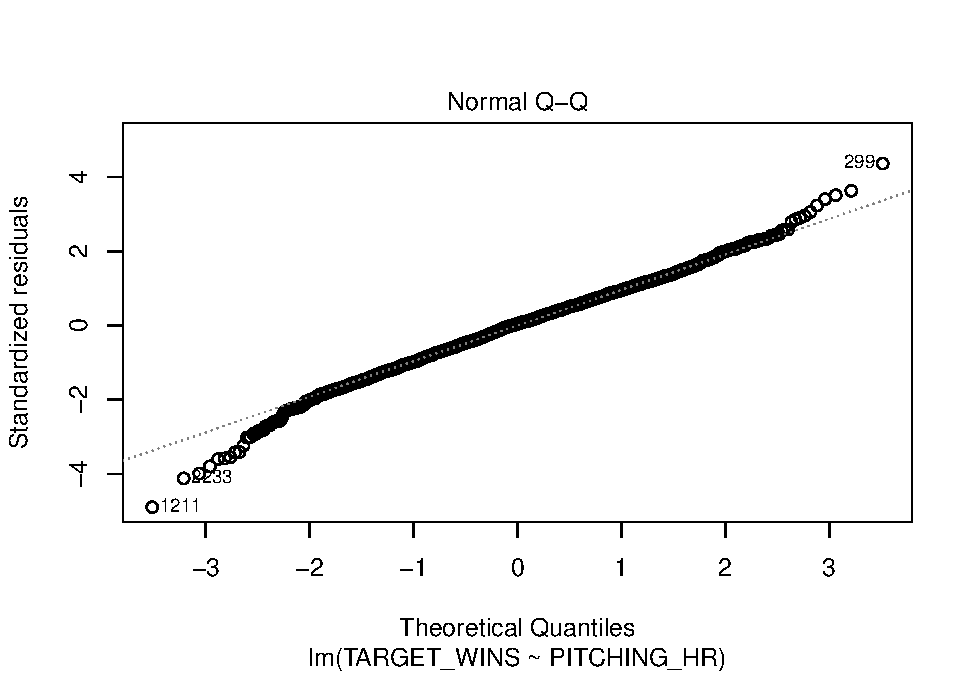
\includegraphics{Baseball5_files/figure-latex/unnamed-chunk-19-2.pdf}
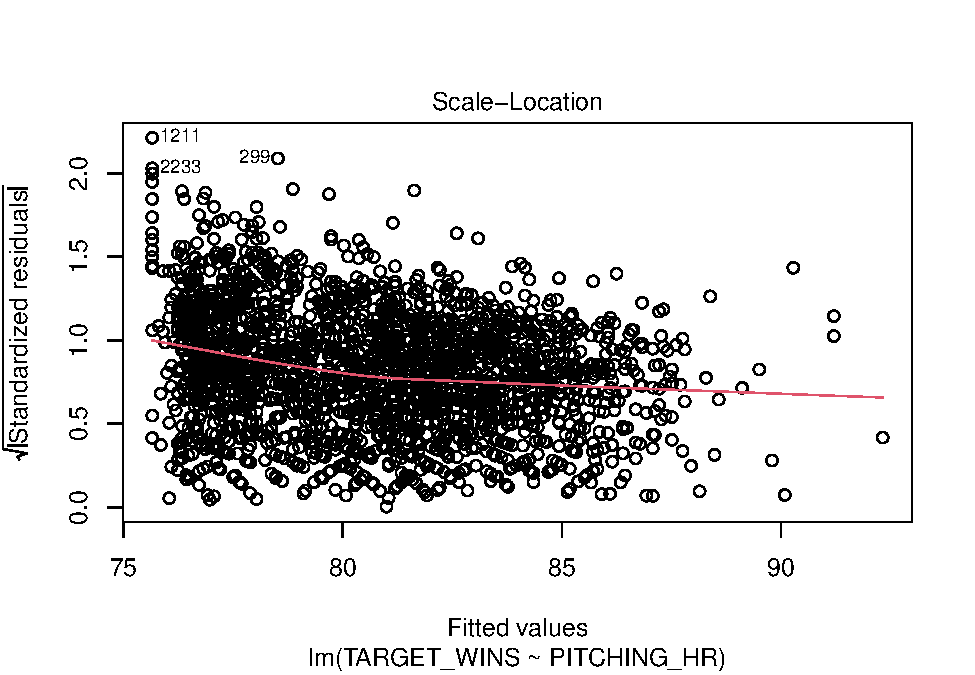
\includegraphics{Baseball5_files/figure-latex/unnamed-chunk-19-3.pdf}
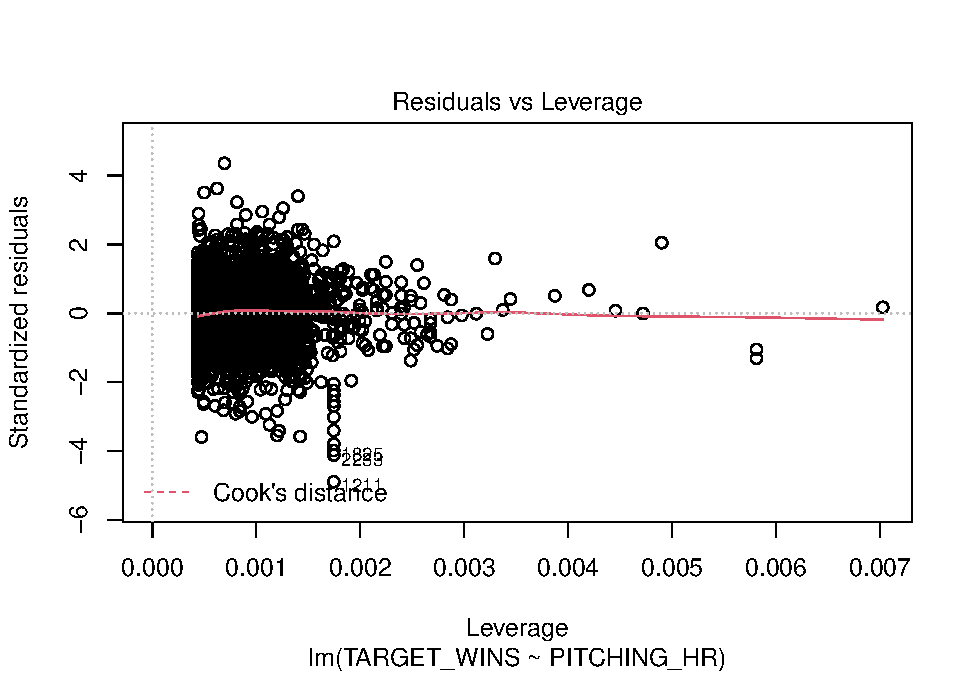
\includegraphics{Baseball5_files/figure-latex/unnamed-chunk-19-4.pdf}

\begin{Shaded}
\begin{Highlighting}[]
\FunctionTok{library}\NormalTok{(car) }
\end{Highlighting}
\end{Shaded}

\begin{verbatim}
## Warning: package 'car' was built under R version 4.0.5
\end{verbatim}

\begin{verbatim}
## Loading required package: carData
\end{verbatim}

\begin{verbatim}
## 
## Attaching package: 'car'
\end{verbatim}

\begin{verbatim}
## The following object is masked from 'package:dplyr':
## 
##     recode
\end{verbatim}

\begin{verbatim}
## The following object is masked from 'package:purrr':
## 
##     some
\end{verbatim}

\begin{verbatim}
## The following object is masked from 'package:psych':
## 
##     logit
\end{verbatim}

\begin{Shaded}
\begin{Highlighting}[]
\FunctionTok{influencePlot}\NormalTok{(m1, }\AttributeTok{id.method=}\StringTok{\textquotesingle{}identify\textquotesingle{}}\NormalTok{, }\AttributeTok{main=}\StringTok{\textquotesingle{}Influence Plot\textquotesingle{}}\NormalTok{, }\AttributeTok{sub=}\StringTok{\textquotesingle{}Circle size is proportional to Cook’s distance\textquotesingle{}}\NormalTok{)}
\end{Highlighting}
\end{Shaded}

\begin{verbatim}
## Warning in plot.window(...): "id.method" is not a graphical parameter
\end{verbatim}

\begin{verbatim}
## Warning in plot.xy(xy, type, ...): "id.method" is not a graphical parameter
\end{verbatim}

\begin{verbatim}
## Warning in axis(side = side, at = at, labels = labels, ...): "id.method" is not
## a graphical parameter

## Warning in axis(side = side, at = at, labels = labels, ...): "id.method" is not
## a graphical parameter
\end{verbatim}

\begin{verbatim}
## Warning in box(...): "id.method" is not a graphical parameter
\end{verbatim}

\begin{verbatim}
## Warning in title(...): "id.method" is not a graphical parameter
\end{verbatim}

\begin{verbatim}
## Warning in plot.xy(xy.coords(x, y), type = type, ...): "id.method" is not a
## graphical parameter
\end{verbatim}

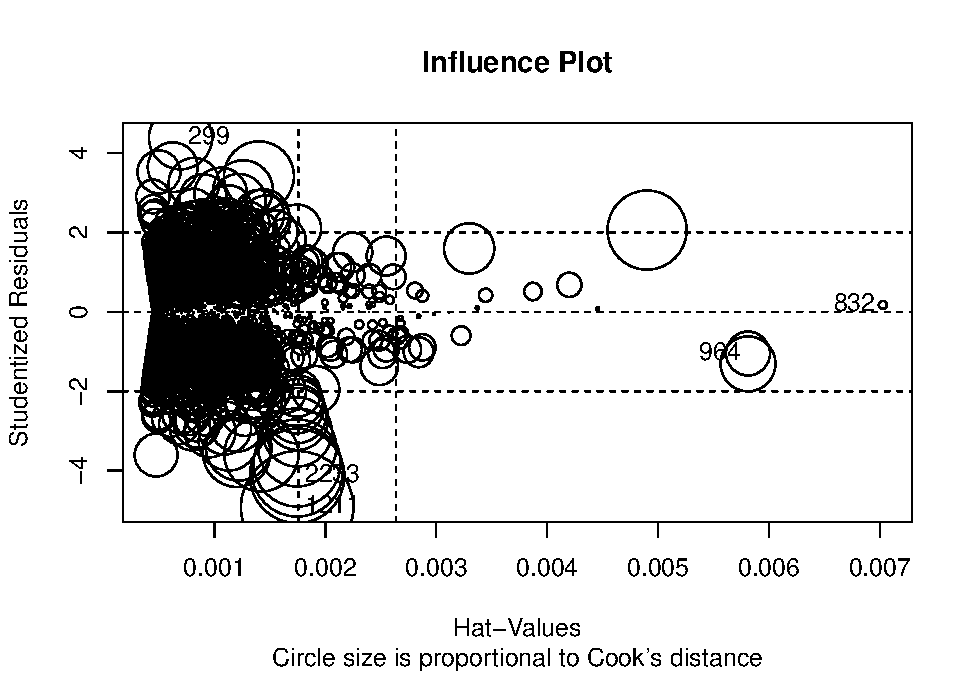
\includegraphics{Baseball5_files/figure-latex/unnamed-chunk-19-5.pdf}

\begin{verbatim}
##        StudRes          Hat        CookD
## 299   4.380293 0.0006944747 0.0066141630
## 832   0.173993 0.0070267976 0.0001071615
## 964  -1.050146 0.0058117315 0.0032231964
## 1211 -4.919225 0.0017463018 0.0209523937
## 2233 -4.132563 0.0017463018 0.0148329515
\end{verbatim}

\begin{Shaded}
\begin{Highlighting}[]
\NormalTok{dfTrain2 }\OtherTok{\textless{}{-}}\NormalTok{ dfTrain[}\SpecialCharTok{{-}}\FunctionTok{c}\NormalTok{(}\DecValTok{1211}\NormalTok{,}\DecValTok{2233}\NormalTok{,}\DecValTok{299}\NormalTok{,}\DecValTok{1825}\NormalTok{, }\DecValTok{832}\NormalTok{), ]}
\FunctionTok{cor.test}\NormalTok{(dfTrain2}\SpecialCharTok{$}\NormalTok{PITCHING\_HR, dfTrain2}\SpecialCharTok{$}\NormalTok{TARGET\_WINS)}
\end{Highlighting}
\end{Shaded}

\begin{verbatim}
## 
##  Pearson's product-moment correlation
## 
## data:  dfTrain2$PITCHING_HR and dfTrain2$TARGET_WINS
## t = 8.8525, df = 2269, p-value < 2.2e-16
## alternative hypothesis: true correlation is not equal to 0
## 95 percent confidence interval:
##  0.1426547 0.2221771
## sample estimates:
##       cor 
## 0.1827147
\end{verbatim}

\begin{Shaded}
\begin{Highlighting}[]
\NormalTok{m2 }\OtherTok{\textless{}{-}} \FunctionTok{lm}\NormalTok{(TARGET\_WINS }\SpecialCharTok{\textasciitilde{}}\NormalTok{ PITCHING\_HR, }\AttributeTok{data=}\NormalTok{dfTrain2)}
\FunctionTok{summary}\NormalTok{(m2)}
\end{Highlighting}
\end{Shaded}

\begin{verbatim}
## 
## Call:
## lm(formula = TARGET_WINS ~ PITCHING_HR, data = dfTrain2)
## 
## Residuals:
##     Min      1Q  Median      3Q     Max 
## -58.949  -9.929   0.614  10.028  55.992 
## 
## Coefficients:
##              Estimate Std. Error t value Pr(>|t|)    
## (Intercept) 75.948820   0.639361 118.789   <2e-16 ***
## PITCHING_HR  0.046356   0.005237   8.852   <2e-16 ***
## ---
## Signif. codes:  0 '***' 0.001 '**' 0.01 '*' 0.05 '.' 0.1 ' ' 1
## 
## Residual standard error: 15.23 on 2269 degrees of freedom
## Multiple R-squared:  0.03338,    Adjusted R-squared:  0.03296 
## F-statistic: 78.37 on 1 and 2269 DF,  p-value: < 2.2e-16
\end{verbatim}

\begin{Shaded}
\begin{Highlighting}[]
\FunctionTok{plot}\NormalTok{(m2)}
\end{Highlighting}
\end{Shaded}

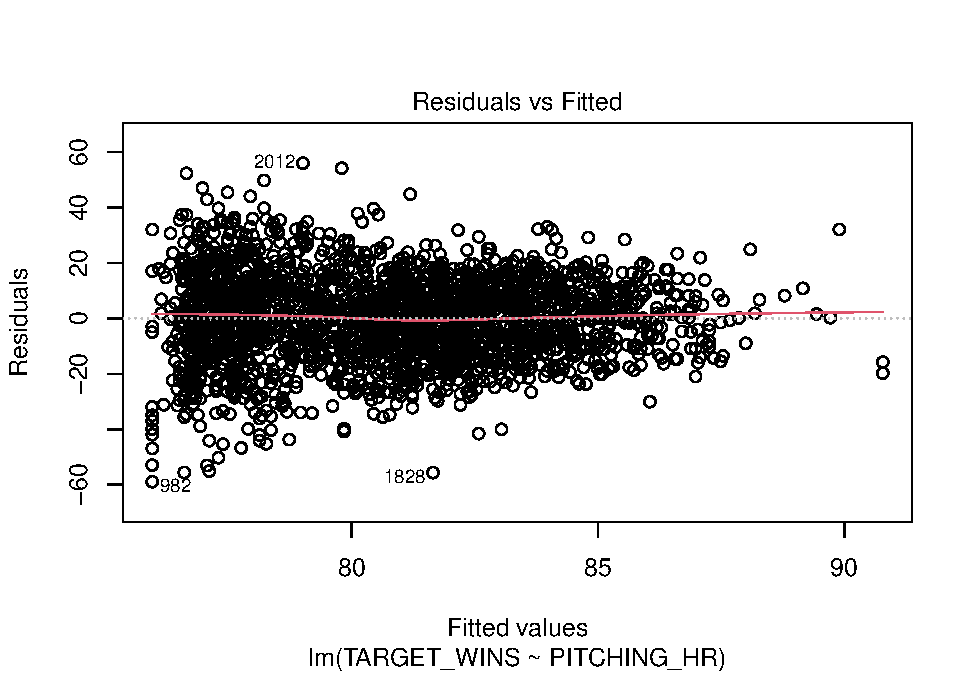
\includegraphics{Baseball5_files/figure-latex/unnamed-chunk-20-1.pdf}
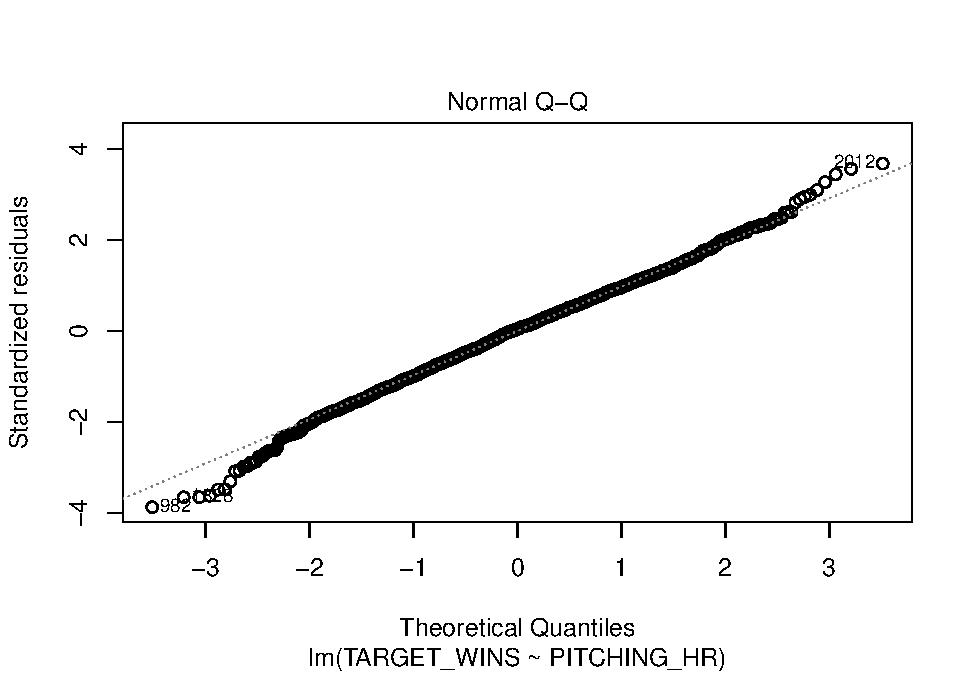
\includegraphics{Baseball5_files/figure-latex/unnamed-chunk-20-2.pdf}
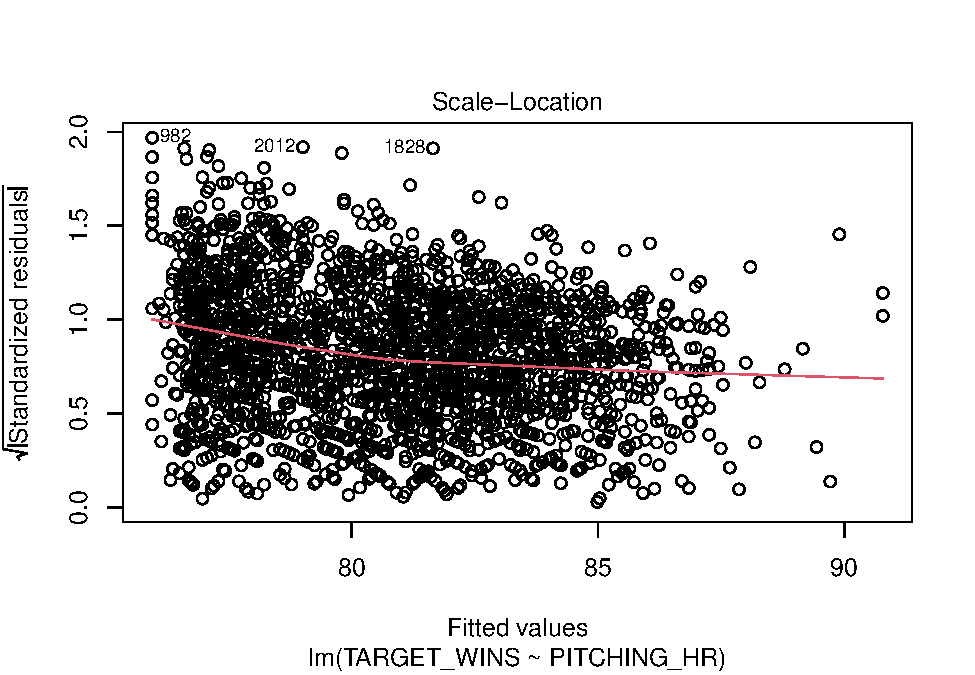
\includegraphics{Baseball5_files/figure-latex/unnamed-chunk-20-3.pdf}
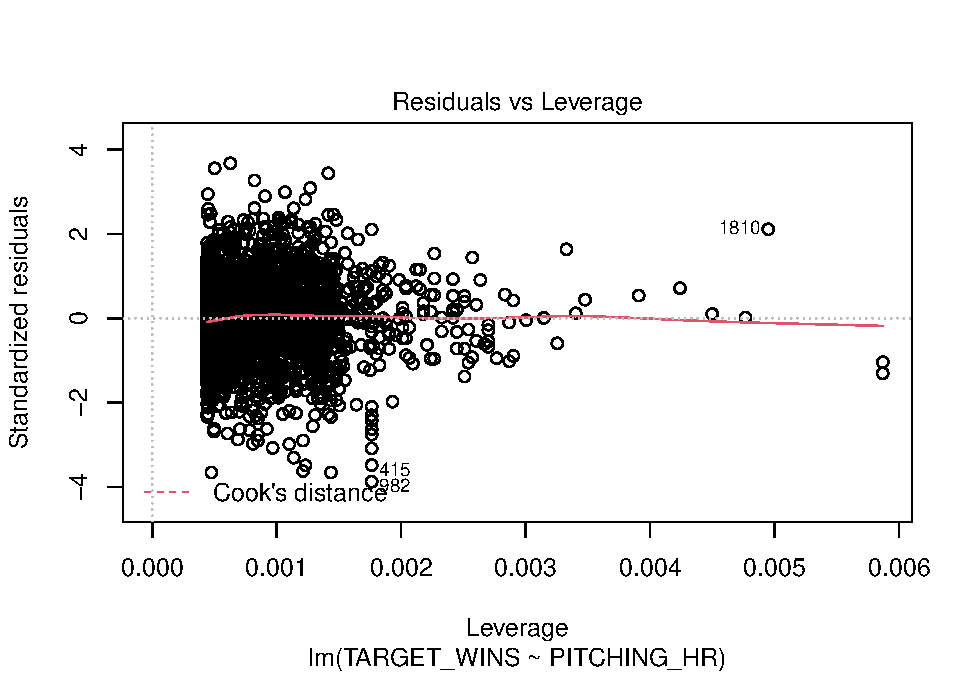
\includegraphics{Baseball5_files/figure-latex/unnamed-chunk-20-4.pdf}

\begin{Shaded}
\begin{Highlighting}[]
\FunctionTok{library}\NormalTok{(car) }
\FunctionTok{influencePlot}\NormalTok{(m2, }\AttributeTok{id.method=}\StringTok{\textquotesingle{}identify\textquotesingle{}}\NormalTok{, }\AttributeTok{main=}\StringTok{\textquotesingle{}Influence Plot\textquotesingle{}}\NormalTok{, }\AttributeTok{sub=}\StringTok{\textquotesingle{}Circle size is proportional to Cook’s distance\textquotesingle{}}\NormalTok{)}
\end{Highlighting}
\end{Shaded}

\begin{verbatim}
## Warning in plot.window(...): "id.method" is not a graphical parameter
\end{verbatim}

\begin{verbatim}
## Warning in plot.xy(xy, type, ...): "id.method" is not a graphical parameter
\end{verbatim}

\begin{verbatim}
## Warning in axis(side = side, at = at, labels = labels, ...): "id.method" is not
## a graphical parameter

## Warning in axis(side = side, at = at, labels = labels, ...): "id.method" is not
## a graphical parameter
\end{verbatim}

\begin{verbatim}
## Warning in box(...): "id.method" is not a graphical parameter
\end{verbatim}

\begin{verbatim}
## Warning in title(...): "id.method" is not a graphical parameter
\end{verbatim}

\begin{verbatim}
## Warning in plot.xy(xy.coords(x, y), type = type, ...): "id.method" is not a
## graphical parameter
\end{verbatim}

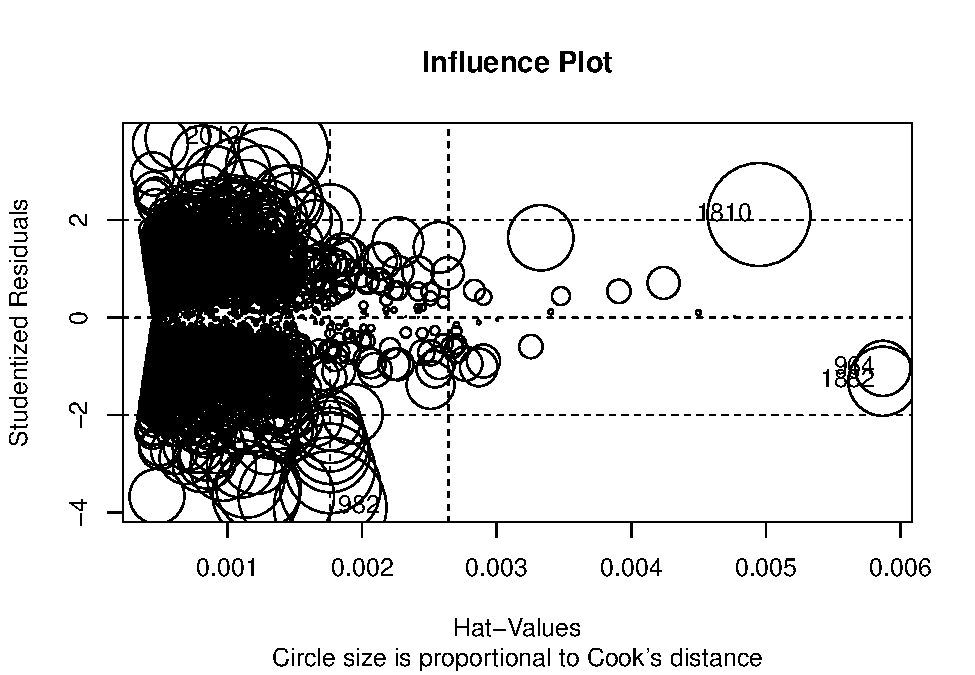
\includegraphics{Baseball5_files/figure-latex/unnamed-chunk-20-5.pdf}

\begin{verbatim}
##        StudRes          Hat       CookD
## 964  -1.039523 0.0058683344 0.003189286
## 982  -3.886600 0.0017628831 0.013255859
## 1810  2.114722 0.0049482791 0.011102505
## 1882 -1.303158 0.0058683344 0.005010737
## 2012  3.688318 0.0006272236 0.004245374
\end{verbatim}

\begin{Shaded}
\begin{Highlighting}[]
\FunctionTok{summary}\NormalTok{(m1}\SpecialCharTok{$}\NormalTok{residuals)}
\end{Highlighting}
\end{Shaded}

\begin{verbatim}
##     Min.  1st Qu.   Median     Mean  3rd Qu.     Max. 
## -75.6569  -9.9562   0.6359   0.0000  10.0552  67.4774
\end{verbatim}

\begin{Shaded}
\begin{Highlighting}[]
\FunctionTok{describe}\NormalTok{(m1}\SpecialCharTok{$}\NormalTok{residuals)}
\end{Highlighting}
\end{Shaded}

\begin{verbatim}
##    vars    n mean    sd median trimmed   mad    min   max  range  skew kurtosis
## X1    1 2276    0 15.47   0.64     0.2 14.84 -75.66 67.48 143.13 -0.18     0.86
##      se
## X1 0.32
\end{verbatim}

\begin{Shaded}
\begin{Highlighting}[]
\NormalTok{dfTrain}\SpecialCharTok{$}\NormalTok{Residuals }\OtherTok{\textless{}{-}}\NormalTok{ m1}\SpecialCharTok{$}\NormalTok{residuals}
\NormalTok{dfTrain}\SpecialCharTok{$}\NormalTok{Fitted }\OtherTok{\textless{}{-}}\NormalTok{ m1}\SpecialCharTok{$}\NormalTok{fitted.values}
\end{Highlighting}
\end{Shaded}

\begin{Shaded}
\begin{Highlighting}[]
\FunctionTok{library}\NormalTok{(tidyverse)}
\end{Highlighting}
\end{Shaded}

\begin{Shaded}
\begin{Highlighting}[]
\NormalTok{dfTrain\_WithoutHR }\OtherTok{\textless{}{-}}\NormalTok{ dfTrain }\SpecialCharTok{\%\textgreater{}\%}
\NormalTok{  dplyr}\SpecialCharTok{::}\FunctionTok{filter}\NormalTok{(TARGET\_WINS }\SpecialCharTok{\textgreater{}=}\DecValTok{50} \SpecialCharTok{|}\NormalTok{ PITCHING\_HR}\SpecialCharTok{!=}\DecValTok{0}\NormalTok{)}

\FunctionTok{hist}\NormalTok{(dfTrain\_WithoutHR}\SpecialCharTok{$}\NormalTok{PITCHING\_HR)}
\end{Highlighting}
\end{Shaded}

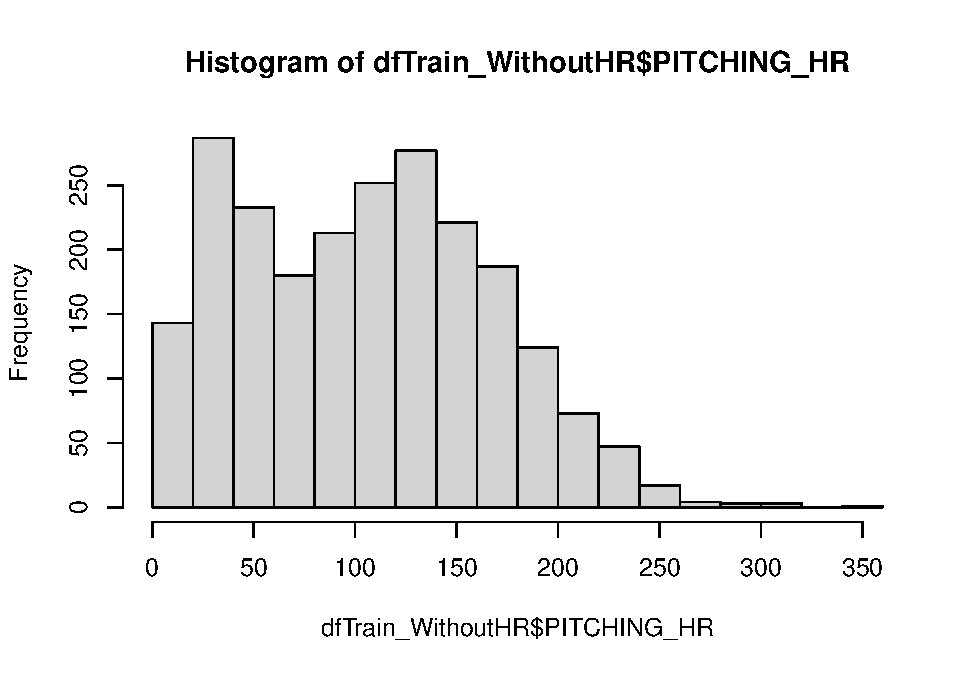
\includegraphics{Baseball5_files/figure-latex/unnamed-chunk-24-1.pdf}

\begin{Shaded}
\begin{Highlighting}[]
\FunctionTok{plot}\NormalTok{(dfTrain\_WithoutHR}\SpecialCharTok{$}\NormalTok{PITCHING\_HR, dfTrain\_WithoutHR}\SpecialCharTok{$}\NormalTok{TARGET\_WINS)}
\end{Highlighting}
\end{Shaded}

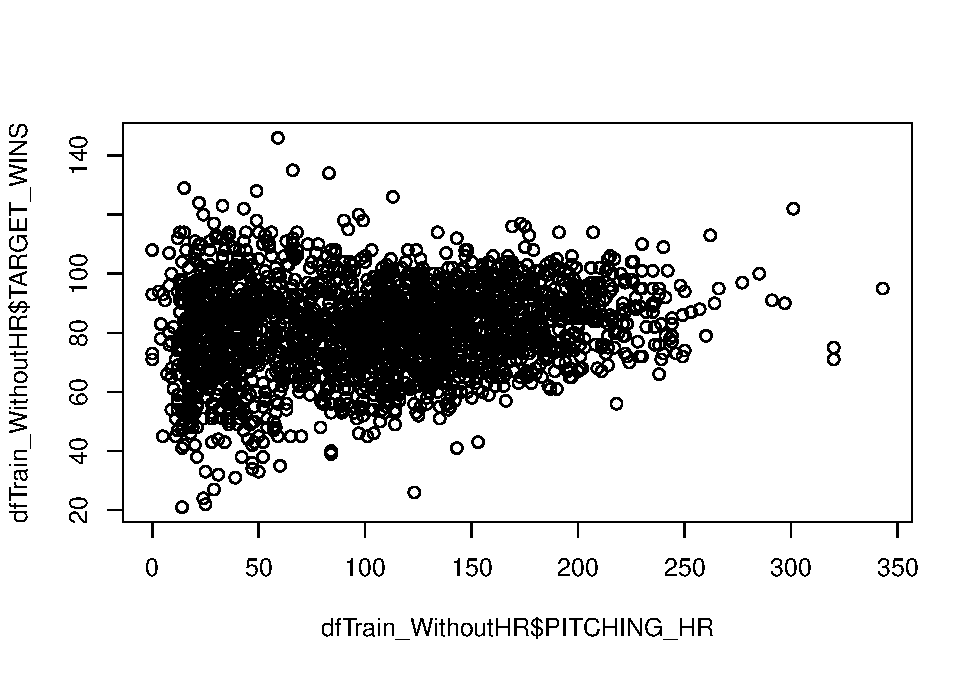
\includegraphics{Baseball5_files/figure-latex/unnamed-chunk-24-2.pdf}

\begin{Shaded}
\begin{Highlighting}[]
\NormalTok{m3 }\OtherTok{\textless{}{-}} \FunctionTok{lm}\NormalTok{(TARGET\_WINS }\SpecialCharTok{\textasciitilde{}}\NormalTok{ PITCHING\_HR, }\AttributeTok{data=}\NormalTok{dfTrain\_WithoutHR)}
\FunctionTok{summary}\NormalTok{(m3)}
\end{Highlighting}
\end{Shaded}

\begin{verbatim}
## 
## Call:
## lm(formula = TARGET_WINS ~ PITCHING_HR, data = dfTrain_WithoutHR)
## 
## Residuals:
##     Min      1Q  Median      3Q     Max 
## -56.208  -9.802   0.653   9.952  66.914 
## 
## Coefficients:
##              Estimate Std. Error t value Pr(>|t|)    
## (Intercept) 76.624136   0.636539 120.376  < 2e-16 ***
## PITCHING_HR  0.041723   0.005197   8.028 1.58e-15 ***
## ---
## Signif. codes:  0 '***' 0.001 '**' 0.01 '*' 0.05 '.' 0.1 ' ' 1
## 
## Residual standard error: 15.09 on 2263 degrees of freedom
## Multiple R-squared:  0.02769,    Adjusted R-squared:  0.02726 
## F-statistic: 64.45 on 1 and 2263 DF,  p-value: 1.576e-15
\end{verbatim}

\begin{Shaded}
\begin{Highlighting}[]
\FunctionTok{plot}\NormalTok{(m3)}
\end{Highlighting}
\end{Shaded}

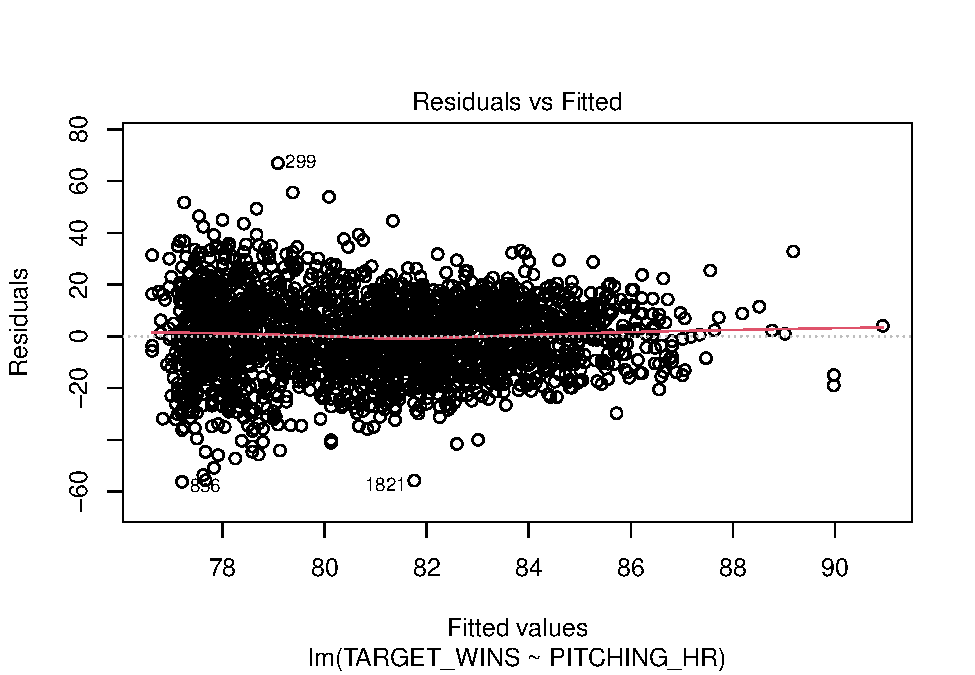
\includegraphics{Baseball5_files/figure-latex/unnamed-chunk-24-3.pdf}
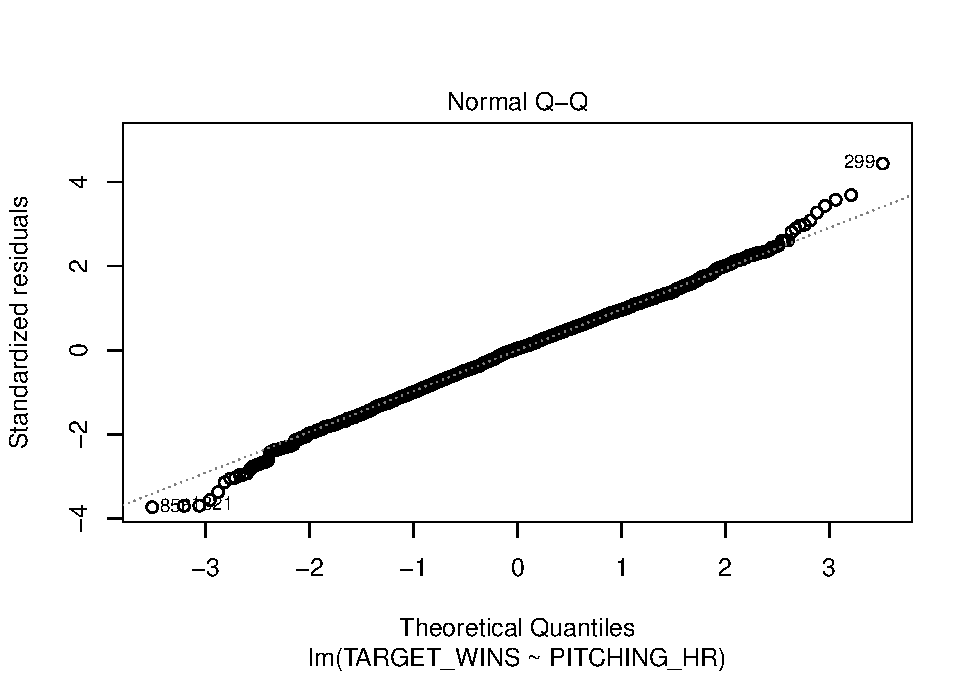
\includegraphics{Baseball5_files/figure-latex/unnamed-chunk-24-4.pdf}
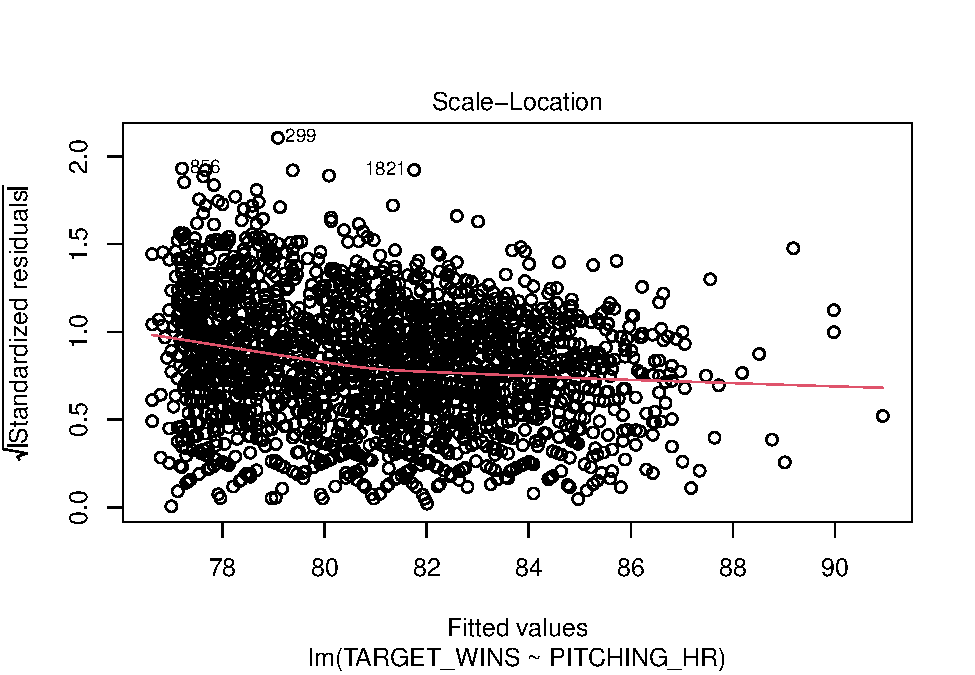
\includegraphics{Baseball5_files/figure-latex/unnamed-chunk-24-5.pdf}
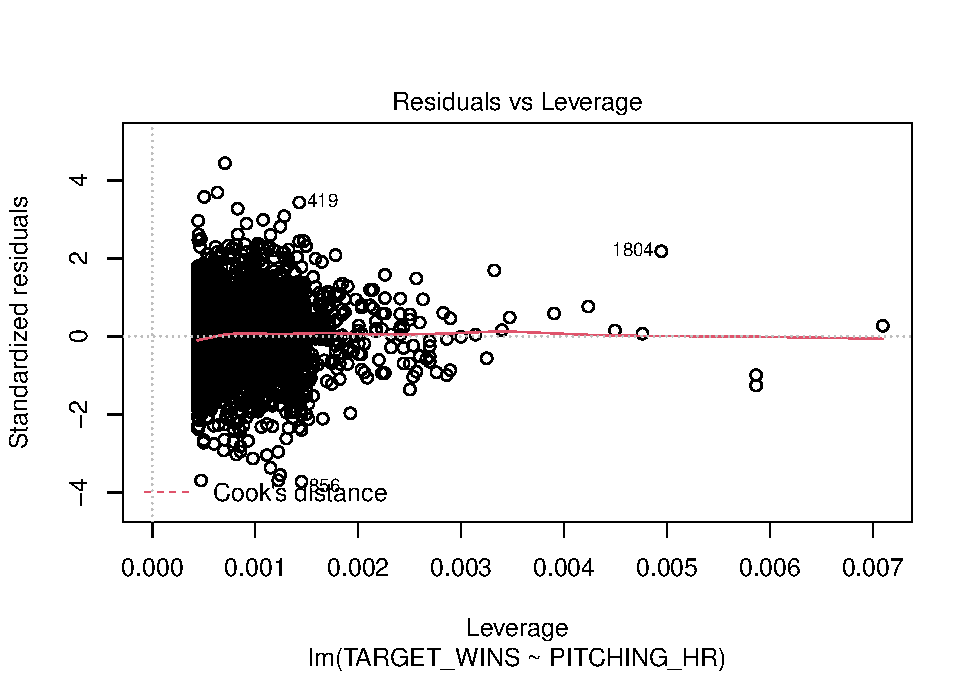
\includegraphics{Baseball5_files/figure-latex/unnamed-chunk-24-6.pdf}

\begin{Shaded}
\begin{Highlighting}[]
\FunctionTok{library}\NormalTok{(car) }
\FunctionTok{influencePlot}\NormalTok{(m3, }\AttributeTok{id.method=}\StringTok{\textquotesingle{}identify\textquotesingle{}}\NormalTok{, }\AttributeTok{main=}\StringTok{\textquotesingle{}Influence Plot\textquotesingle{}}\NormalTok{, }\AttributeTok{sub=}\StringTok{\textquotesingle{}Circle size is proportional to Cook’s distance\textquotesingle{}}\NormalTok{)}
\end{Highlighting}
\end{Shaded}

\begin{verbatim}
## Warning in plot.window(...): "id.method" is not a graphical parameter
\end{verbatim}

\begin{verbatim}
## Warning in plot.xy(xy, type, ...): "id.method" is not a graphical parameter
\end{verbatim}

\begin{verbatim}
## Warning in axis(side = side, at = at, labels = labels, ...): "id.method" is not
## a graphical parameter

## Warning in axis(side = side, at = at, labels = labels, ...): "id.method" is not
## a graphical parameter
\end{verbatim}

\begin{verbatim}
## Warning in box(...): "id.method" is not a graphical parameter
\end{verbatim}

\begin{verbatim}
## Warning in title(...): "id.method" is not a graphical parameter
\end{verbatim}

\begin{verbatim}
## Warning in plot.xy(xy.coords(x, y), type = type, ...): "id.method" is not a
## graphical parameter
\end{verbatim}

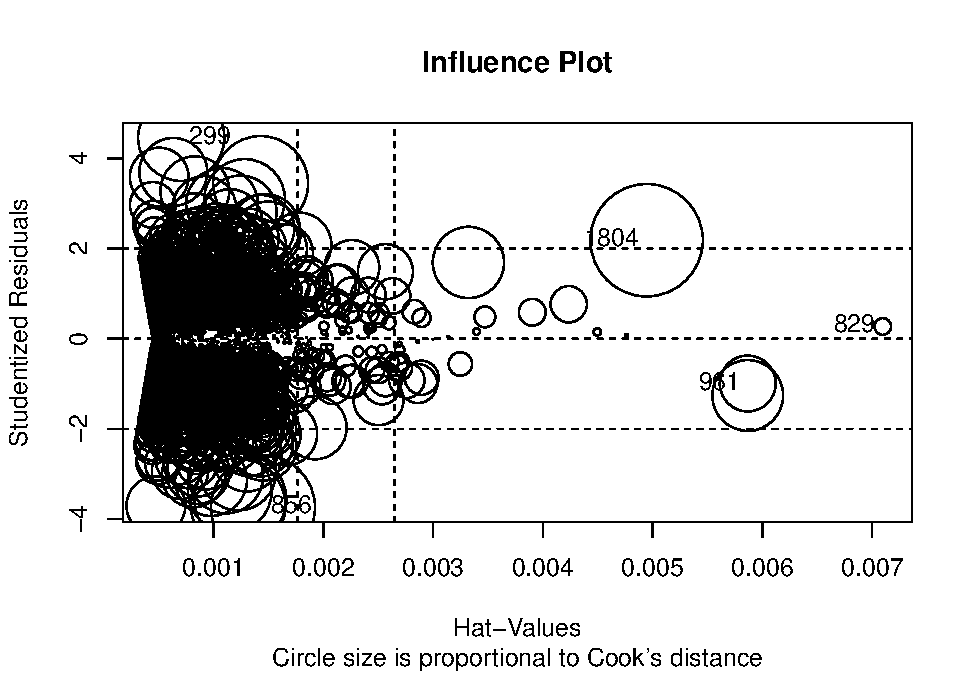
\includegraphics{Baseball5_files/figure-latex/unnamed-chunk-24-7.pdf}

\begin{verbatim}
##         StudRes          Hat        CookD
## 299   4.4557422 0.0007060697 0.0069560265
## 829   0.2703629 0.0070966028 0.0002613277
## 856  -3.7394216 0.0014507753 0.0101000850
## 961  -0.9956483 0.0058665293 0.0029249611
## 1804  2.1826581 0.0049451007 0.0118181032
\end{verbatim}

\begin{Shaded}
\begin{Highlighting}[]
\NormalTok{dfTrain\_BiModal }\OtherTok{\textless{}{-}}\NormalTok{ dfTrain }\SpecialCharTok{\%\textgreater{}\%}
  \FunctionTok{mutate}\NormalTok{(}\AttributeTok{HR\_Low =} \FunctionTok{if\_else}\NormalTok{(PITCHING\_HR}\SpecialCharTok{\textless{}}\DecValTok{50}\NormalTok{,}\DecValTok{1}\NormalTok{,}\DecValTok{0}\NormalTok{)) }\SpecialCharTok{\%\textgreater{}\%}
  \FunctionTok{mutate}\NormalTok{(}\AttributeTok{HR\_High =} \FunctionTok{if\_else}\NormalTok{(PITCHING\_HR}\SpecialCharTok{\textgreater{}=}\DecValTok{50}\NormalTok{,}\DecValTok{1}\NormalTok{,}\DecValTok{0}\NormalTok{))}

\NormalTok{dfCor\_BiModal }\OtherTok{\textless{}{-}} \FunctionTok{as.data.frame}\NormalTok{(}\FunctionTok{cor}\NormalTok{(dfTrain\_BiModal))}
\end{Highlighting}
\end{Shaded}

\begin{Shaded}
\begin{Highlighting}[]
\NormalTok{m4 }\OtherTok{\textless{}{-}} \FunctionTok{lm}\NormalTok{(TARGET\_WINS }\SpecialCharTok{\textasciitilde{}}\NormalTok{ PITCHING\_HR }\SpecialCharTok{+}\NormalTok{ HR\_Low, }\AttributeTok{data=}\NormalTok{dfTrain\_BiModal)}
\FunctionTok{summary}\NormalTok{(m4)}
\end{Highlighting}
\end{Shaded}

\begin{verbatim}
## 
## Call:
## lm(formula = TARGET_WINS ~ PITCHING_HR + HR_Low, data = dfTrain_BiModal)
## 
## Residuals:
##     Min      1Q  Median      3Q     Max 
## -75.692  -9.976   0.653  10.058  67.556 
## 
## Coefficients:
##              Estimate Std. Error t value Pr(>|t|)    
## (Intercept) 75.529253   1.069339  70.632  < 2e-16 ***
## PITCHING_HR  0.049398   0.007641   6.465 1.24e-10 ***
## HR_Low       0.162504   1.084033   0.150    0.881    
## ---
## Signif. codes:  0 '***' 0.001 '**' 0.01 '*' 0.05 '.' 0.1 ' ' 1
## 
## Residual standard error: 15.47 on 2273 degrees of freedom
## Multiple R-squared:  0.03574,    Adjusted R-squared:  0.03489 
## F-statistic: 42.12 on 2 and 2273 DF,  p-value: < 2.2e-16
\end{verbatim}

\begin{Shaded}
\begin{Highlighting}[]
\FunctionTok{plot}\NormalTok{(m4)}
\end{Highlighting}
\end{Shaded}

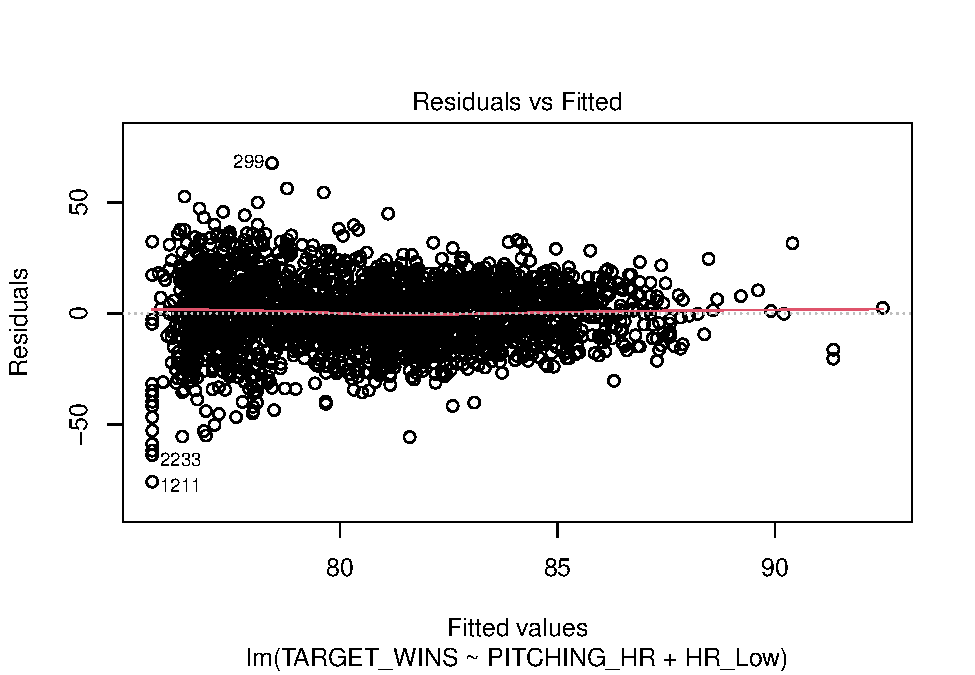
\includegraphics{Baseball5_files/figure-latex/unnamed-chunk-26-1.pdf}
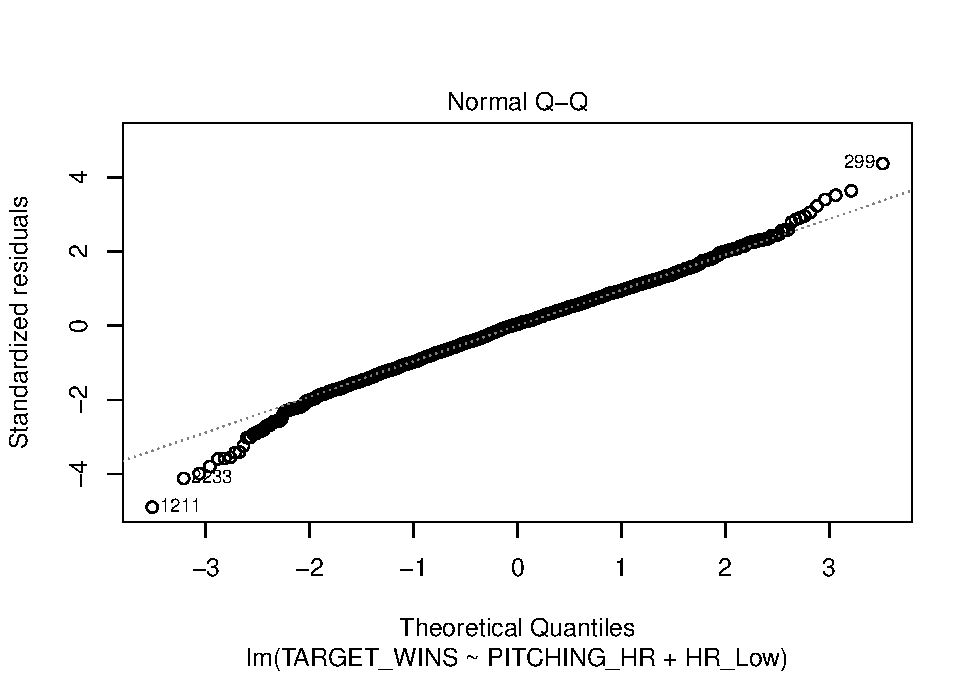
\includegraphics{Baseball5_files/figure-latex/unnamed-chunk-26-2.pdf}
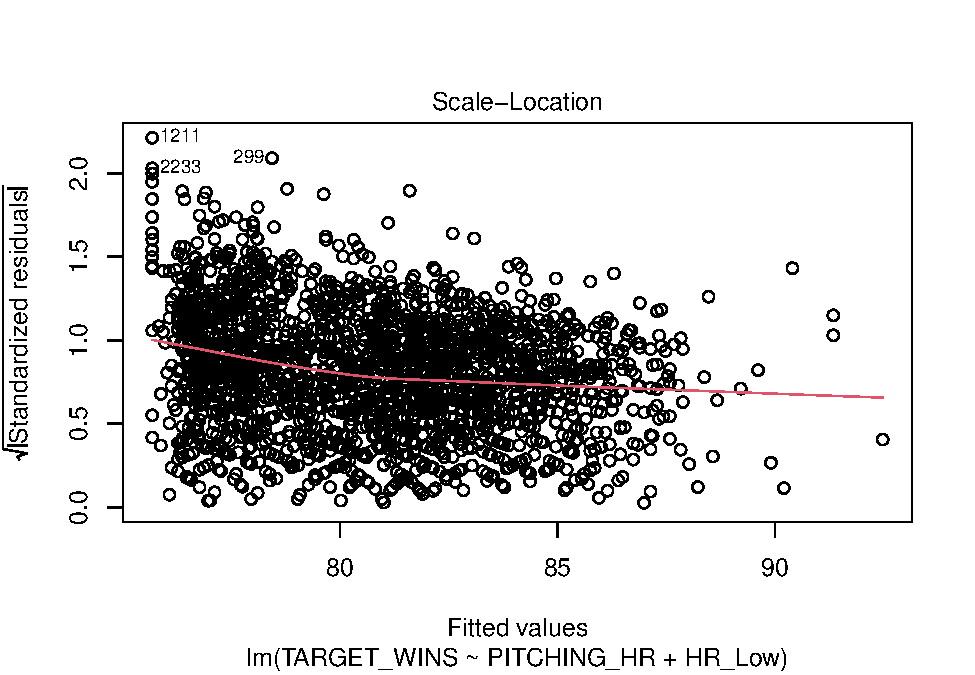
\includegraphics{Baseball5_files/figure-latex/unnamed-chunk-26-3.pdf}
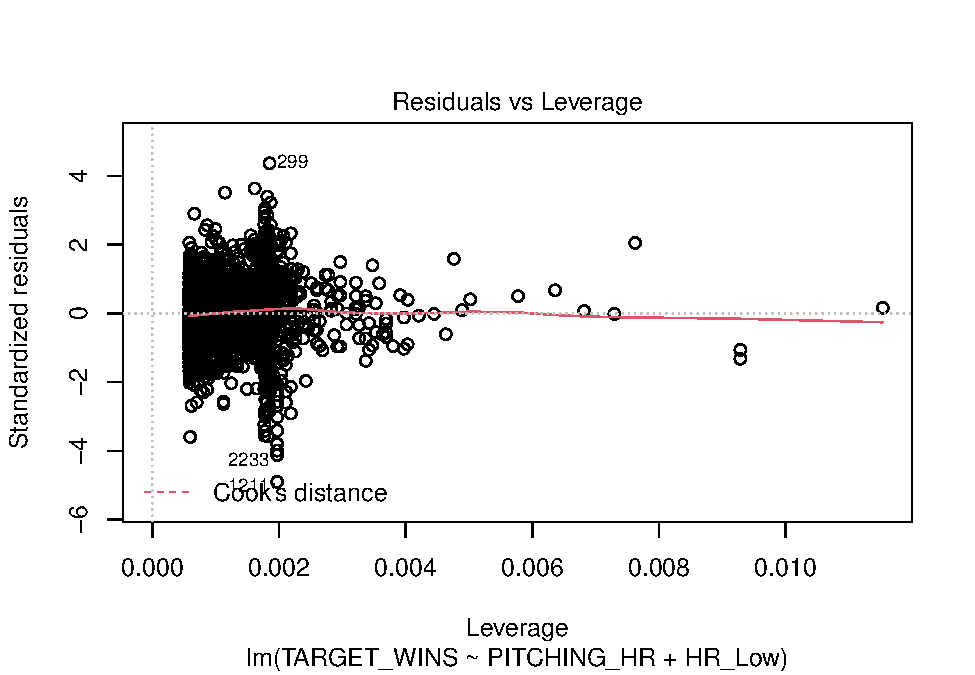
\includegraphics{Baseball5_files/figure-latex/unnamed-chunk-26-4.pdf}

\begin{Shaded}
\begin{Highlighting}[]
\NormalTok{dfHighHR }\OtherTok{\textless{}{-}}\NormalTok{ dfTrain\_BiModal }\SpecialCharTok{\%\textgreater{}\%}
\NormalTok{  dplyr}\SpecialCharTok{::}\FunctionTok{filter}\NormalTok{(HR\_High }\SpecialCharTok{==}\DecValTok{1}\NormalTok{)}

\NormalTok{dfLowHR }\OtherTok{\textless{}{-}}\NormalTok{ dfTrain\_BiModal }\SpecialCharTok{\%\textgreater{}\%}
\NormalTok{  dplyr}\SpecialCharTok{::}\FunctionTok{filter}\NormalTok{(HR\_Low}\SpecialCharTok{==}\DecValTok{1}\NormalTok{)}

\FunctionTok{t.test}\NormalTok{(dfLowHR}\SpecialCharTok{$}\NormalTok{TARGET\_WINS, dfHighHR}\SpecialCharTok{$}\NormalTok{TARGET\_WINS)}
\end{Highlighting}
\end{Shaded}

\begin{verbatim}
## 
##  Welch Two Sample t-test
## 
## data:  dfLowHR$TARGET_WINS and dfHighHR$TARGET_WINS
## t = -5.4141, df = 753, p-value = 8.291e-08
## alternative hypothesis: true difference in means is not equal to 0
## 95 percent confidence interval:
##  -6.665804 -3.118167
## sample estimates:
## mean of x mean of y 
##  77.11327  82.00526
\end{verbatim}

\begin{Shaded}
\begin{Highlighting}[]
\NormalTok{m5 }\OtherTok{\textless{}{-}} \FunctionTok{lm}\NormalTok{(TARGET\_WINS }\SpecialCharTok{\textasciitilde{}}\NormalTok{ PITCHING\_HR, }\AttributeTok{data=}\NormalTok{dfHighHR)}
\FunctionTok{summary}\NormalTok{(m5)}
\end{Highlighting}
\end{Shaded}

\begin{verbatim}
## 
## Call:
## lm(formula = TARGET_WINS ~ PITCHING_HR, data = dfHighHR)
## 
## Residuals:
##     Min      1Q  Median      3Q     Max 
## -55.641  -9.293   0.650   9.127  67.238 
## 
## Coefficients:
##              Estimate Std. Error t value Pr(>|t|)    
## (Intercept) 76.107959   0.957161  79.514  < 2e-16 ***
## PITCHING_HR  0.044983   0.006848   6.569 6.72e-11 ***
## ---
## Signif. codes:  0 '***' 0.001 '**' 0.01 '*' 0.05 '.' 0.1 ' ' 1
## 
## Residual standard error: 13.73 on 1709 degrees of freedom
## Multiple R-squared:  0.02463,    Adjusted R-squared:  0.02405 
## F-statistic: 43.15 on 1 and 1709 DF,  p-value: 6.72e-11
\end{verbatim}

\begin{Shaded}
\begin{Highlighting}[]
\FunctionTok{plot}\NormalTok{(m5)}
\end{Highlighting}
\end{Shaded}

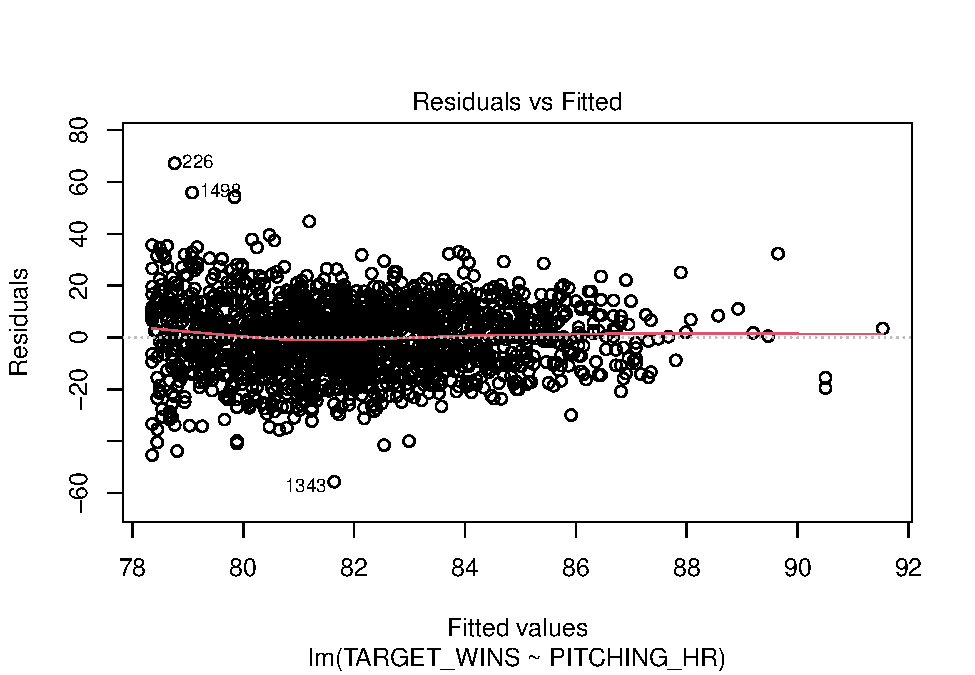
\includegraphics{Baseball5_files/figure-latex/unnamed-chunk-27-1.pdf}
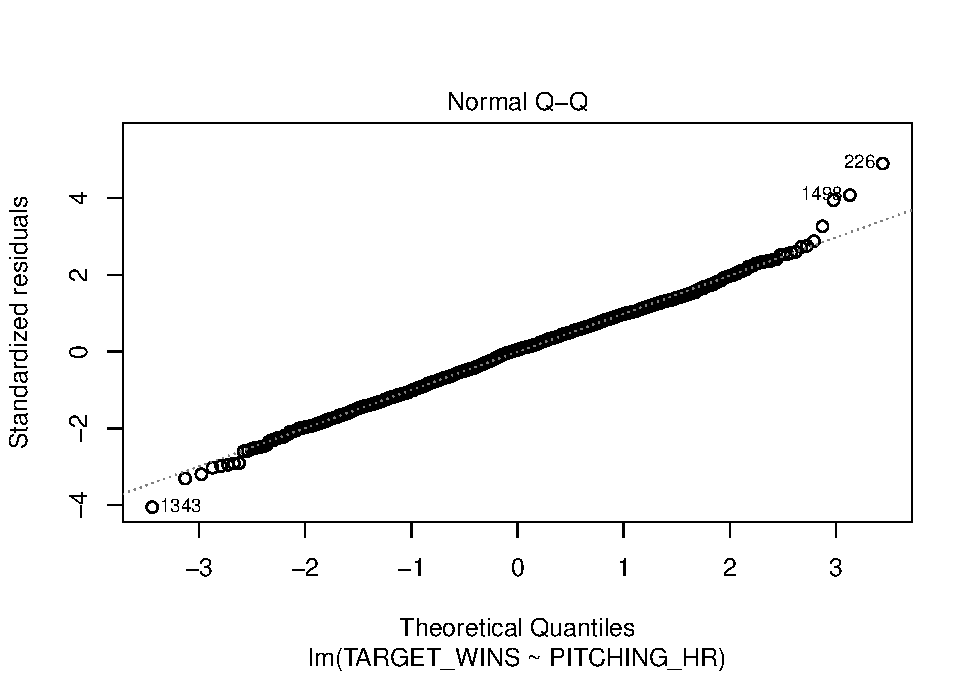
\includegraphics{Baseball5_files/figure-latex/unnamed-chunk-27-2.pdf}
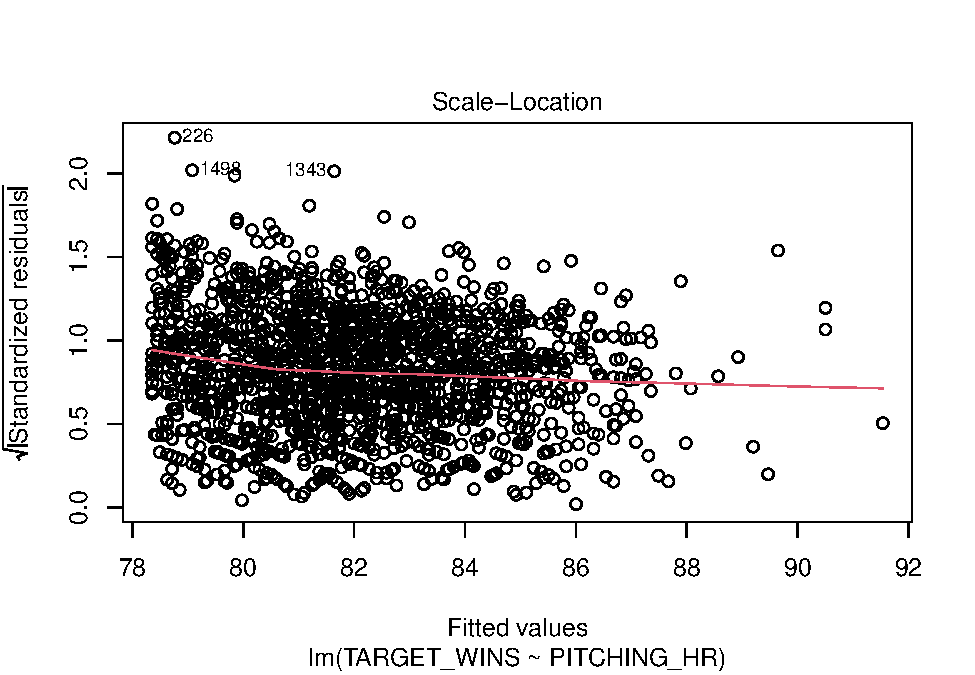
\includegraphics{Baseball5_files/figure-latex/unnamed-chunk-27-3.pdf}
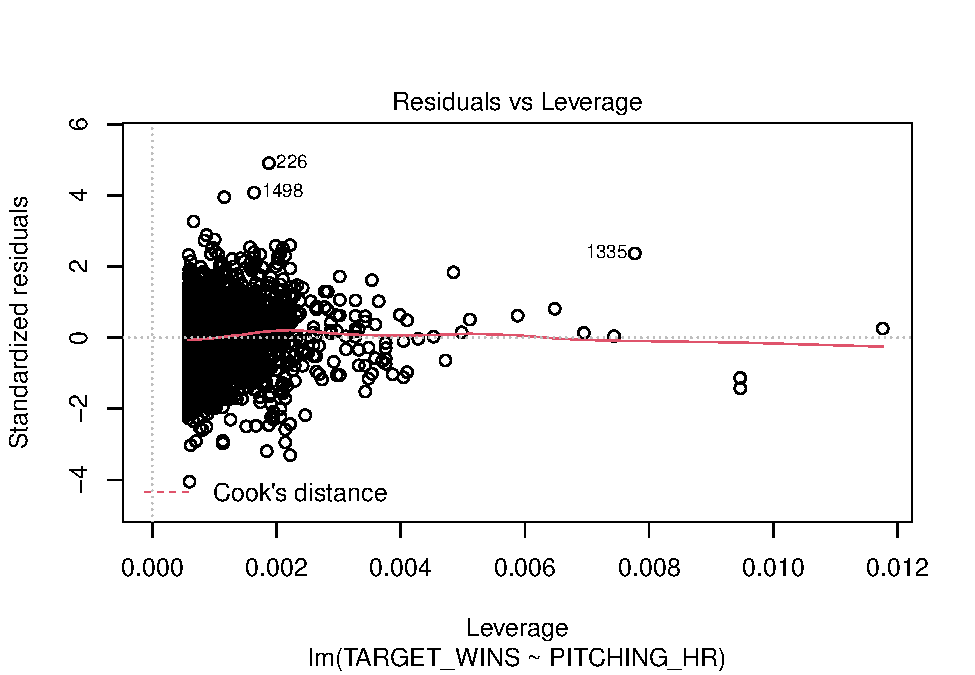
\includegraphics{Baseball5_files/figure-latex/unnamed-chunk-27-4.pdf}

\begin{Shaded}
\begin{Highlighting}[]
\NormalTok{dfCor\_HR }\OtherTok{\textless{}{-}} \FunctionTok{as.data.frame}\NormalTok{(}\FunctionTok{cor}\NormalTok{(dfTrain\_BiModal[}\SpecialCharTok{{-}}\DecValTok{1}\NormalTok{], dfTrain\_BiModal}\SpecialCharTok{$}\NormalTok{PITCHING\_HR)) }
\NormalTok{dfCor\_Low }\OtherTok{\textless{}{-}} \FunctionTok{as.data.frame}\NormalTok{(}\FunctionTok{cor}\NormalTok{(dfTrain\_BiModal[}\SpecialCharTok{{-}}\DecValTok{1}\NormalTok{], dfTrain\_BiModal}\SpecialCharTok{$}\NormalTok{HR\_Low))}

\FunctionTok{plot}\NormalTok{(dfTrain}\SpecialCharTok{$}\NormalTok{BATTING\_HR, dfTrain}\SpecialCharTok{$}\NormalTok{PITCHING\_HR)}
\end{Highlighting}
\end{Shaded}

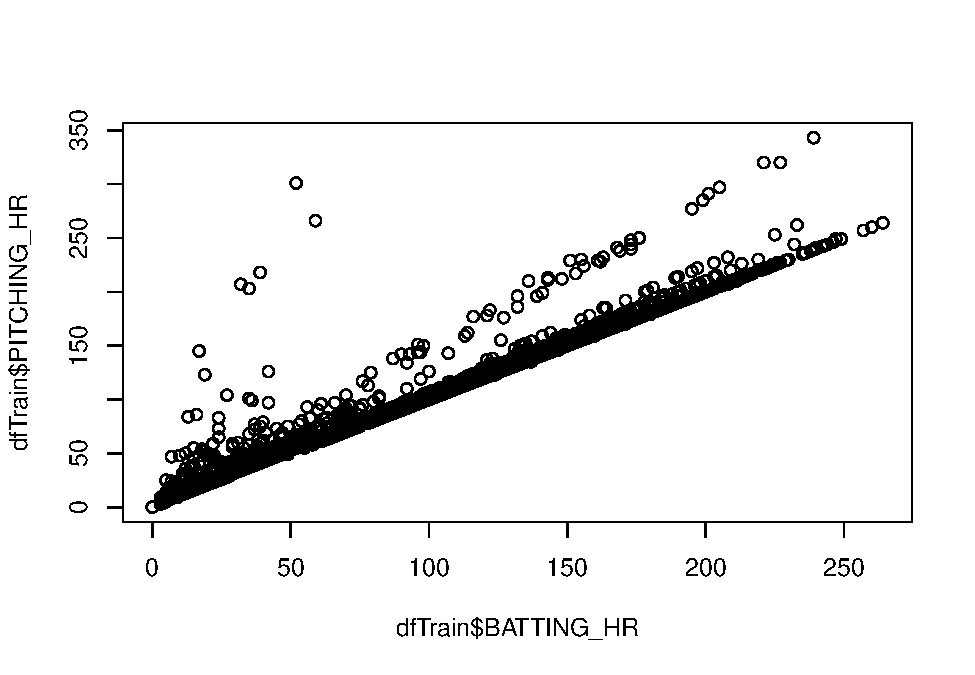
\includegraphics{Baseball5_files/figure-latex/unnamed-chunk-28-1.pdf}

\begin{Shaded}
\begin{Highlighting}[]
\NormalTok{dfTrain}\SpecialCharTok{$}\NormalTok{HR\_Diff }\OtherTok{\textless{}{-}}\NormalTok{ dfTrain}\SpecialCharTok{$}\NormalTok{PITCHING\_HR }\SpecialCharTok{{-}}\NormalTok{dfTrain}\SpecialCharTok{$}\NormalTok{BATTING\_HR}
\FunctionTok{hist}\NormalTok{(dfTrain}\SpecialCharTok{$}\NormalTok{HR\_Diff, }\AttributeTok{breaks=}\DecValTok{100}\NormalTok{)}
\end{Highlighting}
\end{Shaded}

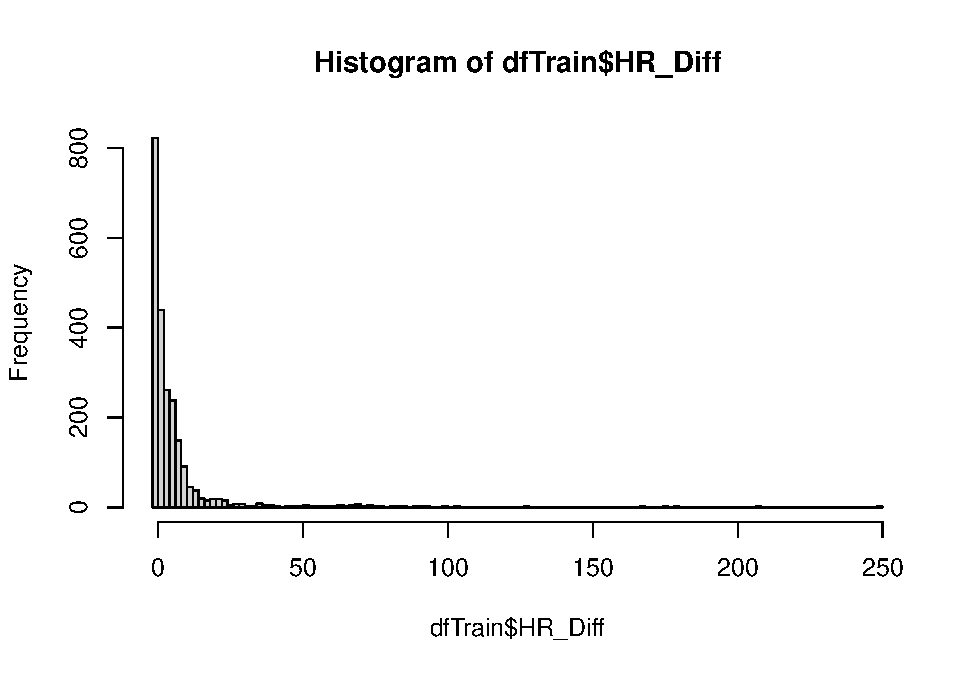
\includegraphics{Baseball5_files/figure-latex/unnamed-chunk-29-1.pdf}

\begin{Shaded}
\begin{Highlighting}[]
\FunctionTok{describe}\NormalTok{(dfTrain}\SpecialCharTok{$}\NormalTok{HR\_Diff)}
\end{Highlighting}
\end{Shaded}

\begin{verbatim}
##    vars    n mean   sd median trimmed  mad min max range skew kurtosis   se
## X1    1 2276 6.09 15.1      2    2.93 2.97  -2 249   251 6.98    71.83 0.32
\end{verbatim}

Sum of HR allowed greatly exceeds sum of HR hit

\begin{Shaded}
\begin{Highlighting}[]
\NormalTok{m6 }\OtherTok{\textless{}{-}} \FunctionTok{lm}\NormalTok{(dfTrain}\SpecialCharTok{$}\NormalTok{BATTING\_HR }\SpecialCharTok{\textasciitilde{}}\NormalTok{ dfTrain}\SpecialCharTok{$}\NormalTok{PITCHING\_HR)}
\FunctionTok{summary}\NormalTok{(m6)}
\end{Highlighting}
\end{Shaded}

\begin{verbatim}
## 
## Call:
## lm(formula = dfTrain$BATTING_HR ~ dfTrain$PITCHING_HR)
## 
## Residuals:
##      Min       1Q   Median       3Q      Max 
## -234.609    0.123    1.336    6.992   12.817 
## 
## Coefficients:
##                      Estimate Std. Error t value Pr(>|t|)    
## (Intercept)         -1.592392   0.621547  -2.562   0.0105 *  
## dfTrain$PITCHING_HR  0.957481   0.005087 188.217   <2e-16 ***
## ---
## Signif. codes:  0 '***' 0.001 '**' 0.01 '*' 0.05 '.' 0.1 ' ' 1
## 
## Residual standard error: 14.87 on 2274 degrees of freedom
## Multiple R-squared:  0.9397, Adjusted R-squared:  0.9397 
## F-statistic: 3.543e+04 on 1 and 2274 DF,  p-value: < 2.2e-16
\end{verbatim}

\begin{Shaded}
\begin{Highlighting}[]
\FunctionTok{plot}\NormalTok{(m6)}
\end{Highlighting}
\end{Shaded}

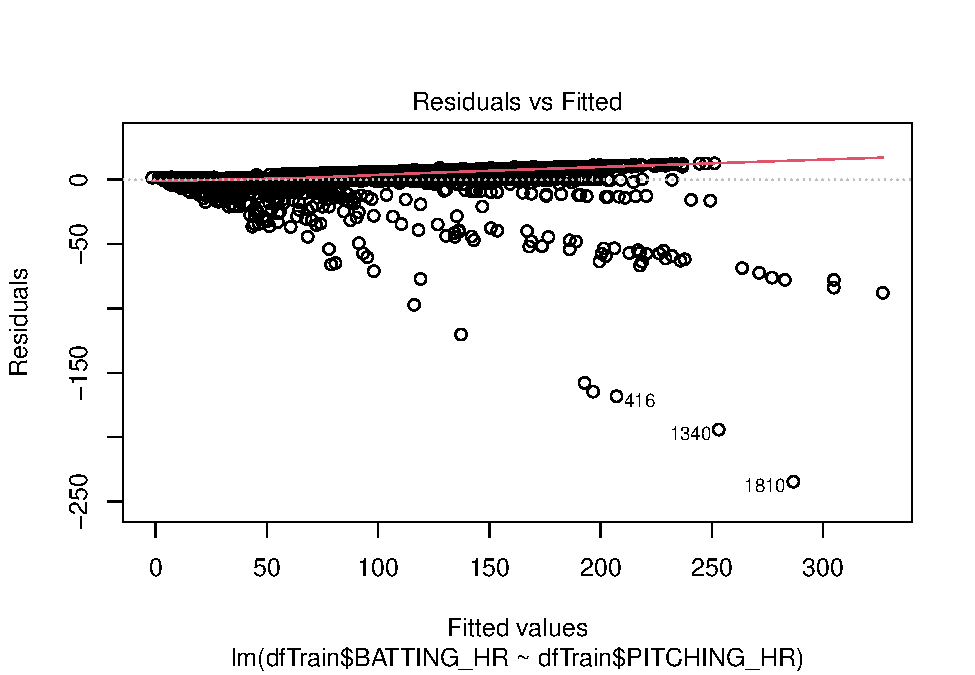
\includegraphics{Baseball5_files/figure-latex/unnamed-chunk-31-1.pdf}
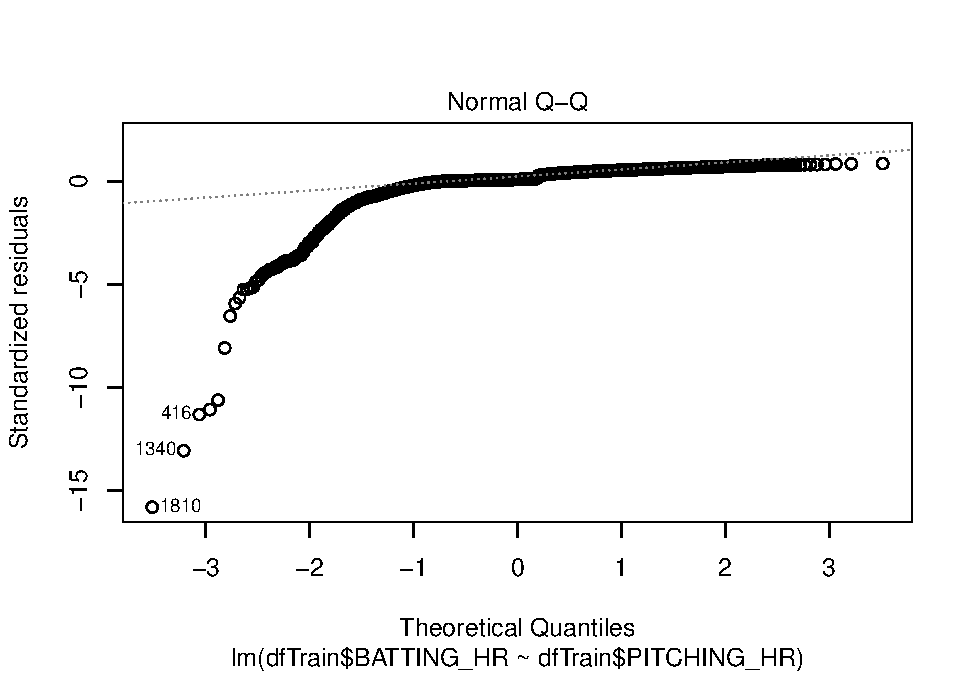
\includegraphics{Baseball5_files/figure-latex/unnamed-chunk-31-2.pdf}
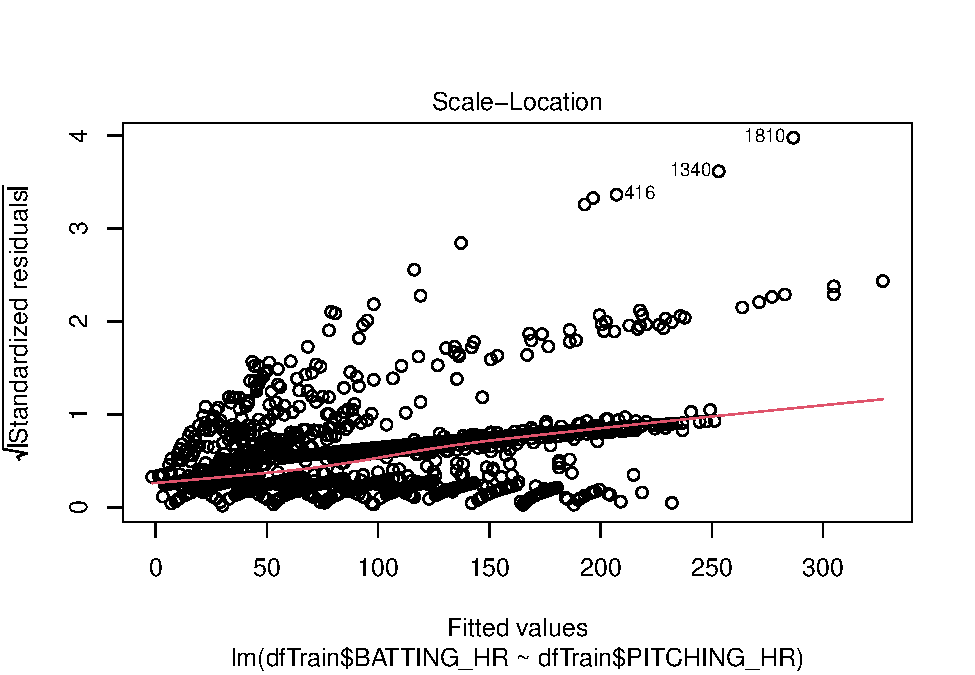
\includegraphics{Baseball5_files/figure-latex/unnamed-chunk-31-3.pdf}
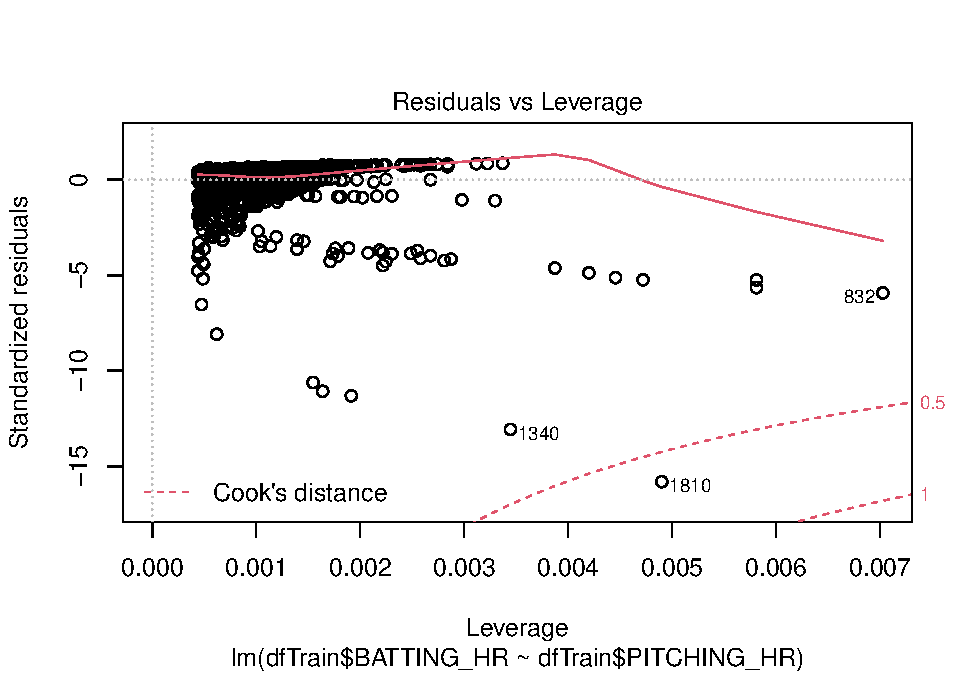
\includegraphics{Baseball5_files/figure-latex/unnamed-chunk-31-4.pdf}

\begin{Shaded}
\begin{Highlighting}[]
\FunctionTok{cor.test}\NormalTok{(dfTrain}\SpecialCharTok{$}\NormalTok{BATTING\_BB, dfTrain}\SpecialCharTok{$}\NormalTok{PITCHING\_BB)}
\end{Highlighting}
\end{Shaded}

\begin{verbatim}
## 
##  Pearson's product-moment correlation
## 
## data:  dfTrain$BATTING_BB and dfTrain$PITCHING_BB
## t = 26.759, df = 2274, p-value < 2.2e-16
## alternative hypothesis: true correlation is not equal to 0
## 95 percent confidence interval:
##  0.4574724 0.5199930
## sample estimates:
##       cor 
## 0.4893613
\end{verbatim}

\begin{Shaded}
\begin{Highlighting}[]
\FunctionTok{plot}\NormalTok{(dfTrain}\SpecialCharTok{$}\NormalTok{BATTING\_BB, dfTrain}\SpecialCharTok{$}\NormalTok{PITCHING\_BB)}
\end{Highlighting}
\end{Shaded}

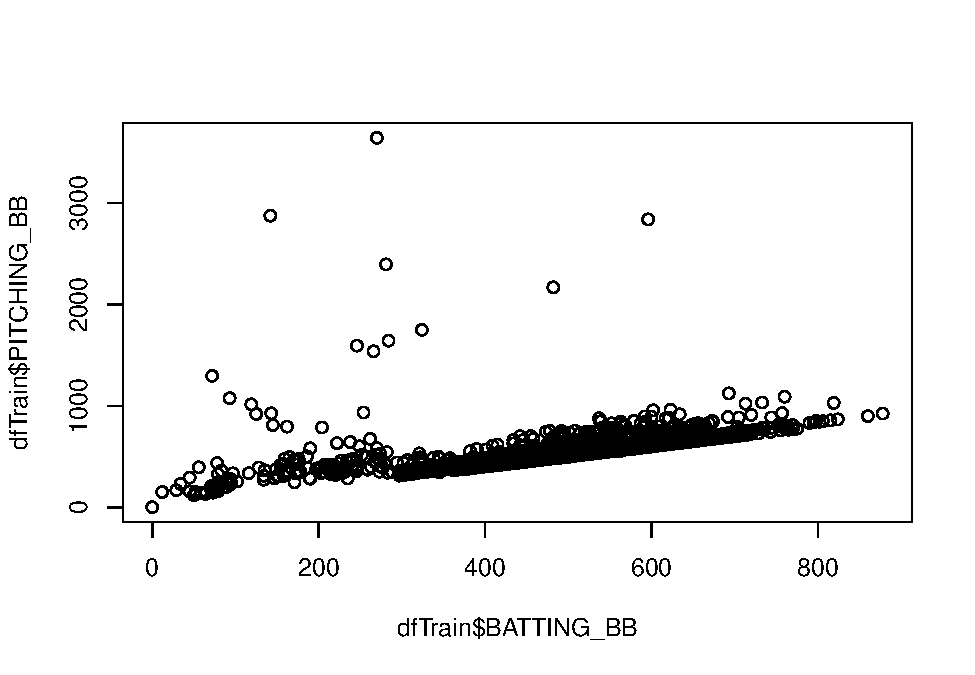
\includegraphics{Baseball5_files/figure-latex/unnamed-chunk-32-1.pdf}

\begin{enumerate}
\def\labelenumi{\alph{enumi}.}
\setcounter{enumi}{2}
\tightlist
\item
  look at relationships with Dependent variable
\end{enumerate}

\begin{Shaded}
\begin{Highlighting}[]
\NormalTok{dfTrain\_ImputedMedian }\OtherTok{\textless{}{-}}\NormalTok{ dfTrain\_ImputedMean\_NoCohort}

\ControlFlowTok{for}\NormalTok{(i }\ControlFlowTok{in} \DecValTok{2}\SpecialCharTok{:}\FunctionTok{ncol}\NormalTok{(dfTrain\_ImputedMedian)) \{                              }
  \FunctionTok{print}\NormalTok{(}\FunctionTok{ggplot}\NormalTok{(dfTrain\_ImputedMedian, }\FunctionTok{aes}\NormalTok{(}\AttributeTok{x =}\NormalTok{ dfTrain\_ImputedMedian[ ,i], }\AttributeTok{y =}\NormalTok{ dfTrain\_ImputedMedian}\SpecialCharTok{$}\NormalTok{TARGET\_WINS)) }\SpecialCharTok{+}
          \FunctionTok{xlab}\NormalTok{(}\FunctionTok{colnames}\NormalTok{(dfTrain)[i])  }\SpecialCharTok{+}
          \FunctionTok{stat\_smooth}\NormalTok{(}\AttributeTok{method=}\NormalTok{loess) }\SpecialCharTok{+}
          \FunctionTok{geom\_point}\NormalTok{())}

\NormalTok{m }\OtherTok{\textless{}{-}} \FunctionTok{lm}\NormalTok{(dfTrain\_ImputedMedian}\SpecialCharTok{$}\NormalTok{TARGET\_WINS }\SpecialCharTok{\textasciitilde{}}\NormalTok{ dfTrain\_ImputedMedian[ ,i])}

\FunctionTok{par}\NormalTok{(}\AttributeTok{mfcol=}\FunctionTok{c}\NormalTok{(}\DecValTok{2}\NormalTok{,}\DecValTok{2}\NormalTok{))}
\FunctionTok{print}\NormalTok{(}\FunctionTok{summary}\NormalTok{(m))}
\FunctionTok{print}\NormalTok{(}\FunctionTok{plot}\NormalTok{(m))}
\NormalTok{\}}
\end{Highlighting}
\end{Shaded}

\begin{verbatim}
## Warning: Use of `dfTrain_ImputedMedian$TARGET_WINS` is discouraged. Use
## `TARGET_WINS` instead.

## Warning: Use of `dfTrain_ImputedMedian$TARGET_WINS` is discouraged. Use
## `TARGET_WINS` instead.
\end{verbatim}

\begin{verbatim}
## `geom_smooth()` using formula 'y ~ x'
\end{verbatim}

\begin{verbatim}
## Warning in summary.lm(m): essentially perfect fit: summary may be unreliable
\end{verbatim}

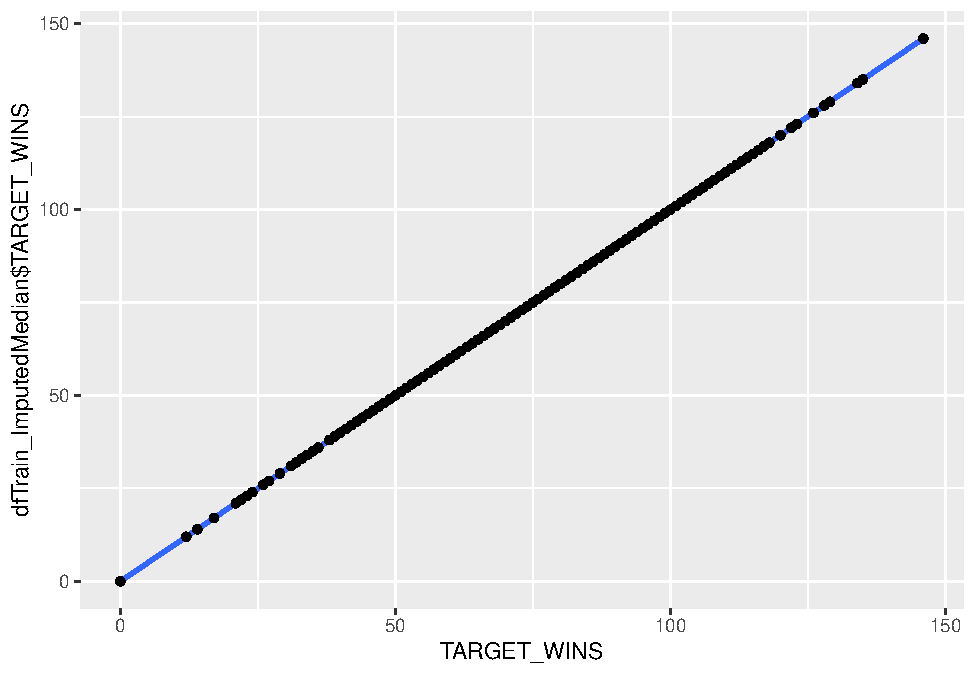
\includegraphics{Baseball5_files/figure-latex/unnamed-chunk-33-1.pdf}

\begin{verbatim}
## 
## Call:
## lm(formula = dfTrain_ImputedMedian$TARGET_WINS ~ dfTrain_ImputedMedian[, 
##     i])
## 
## Residuals:
##        Min         1Q     Median         3Q        Max 
## -3.647e-14 -1.120e-15 -7.000e-16 -2.800e-16  1.614e-12 
## 
## Coefficients:
##                             Estimate Std. Error   t value Pr(>|t|)    
## (Intercept)                1.756e-13  3.928e-15 4.470e+01   <2e-16 ***
## dfTrain_ImputedMedian[, i] 1.000e+00  4.775e-17 2.094e+16   <2e-16 ***
## ---
## Signif. codes:  0 '***' 0.001 '**' 0.01 '*' 0.05 '.' 0.1 ' ' 1
## 
## Residual standard error: 3.467e-14 on 2172 degrees of freedom
## Multiple R-squared:      1,  Adjusted R-squared:      1 
## F-statistic: 4.385e+32 on 1 and 2172 DF,  p-value: < 2.2e-16
\end{verbatim}

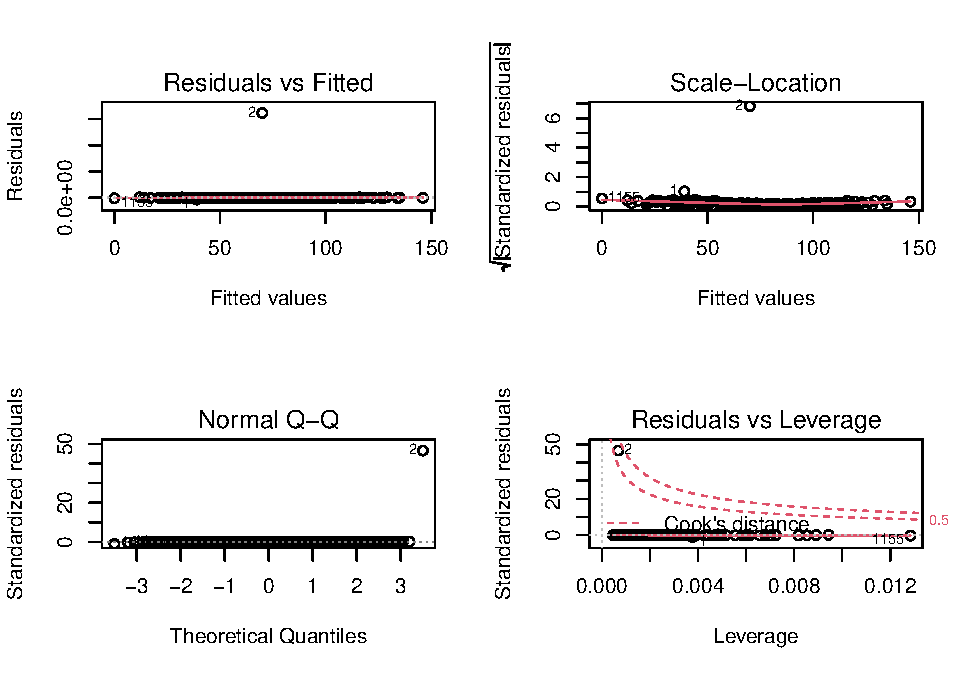
\includegraphics{Baseball5_files/figure-latex/unnamed-chunk-33-2.pdf}

\begin{verbatim}
## NULL
\end{verbatim}

\begin{verbatim}
## Warning: Use of `dfTrain_ImputedMedian$TARGET_WINS` is discouraged. Use
## `TARGET_WINS` instead.

## Warning: Use of `dfTrain_ImputedMedian$TARGET_WINS` is discouraged. Use
## `TARGET_WINS` instead.
\end{verbatim}

\begin{verbatim}
## `geom_smooth()` using formula 'y ~ x'
\end{verbatim}

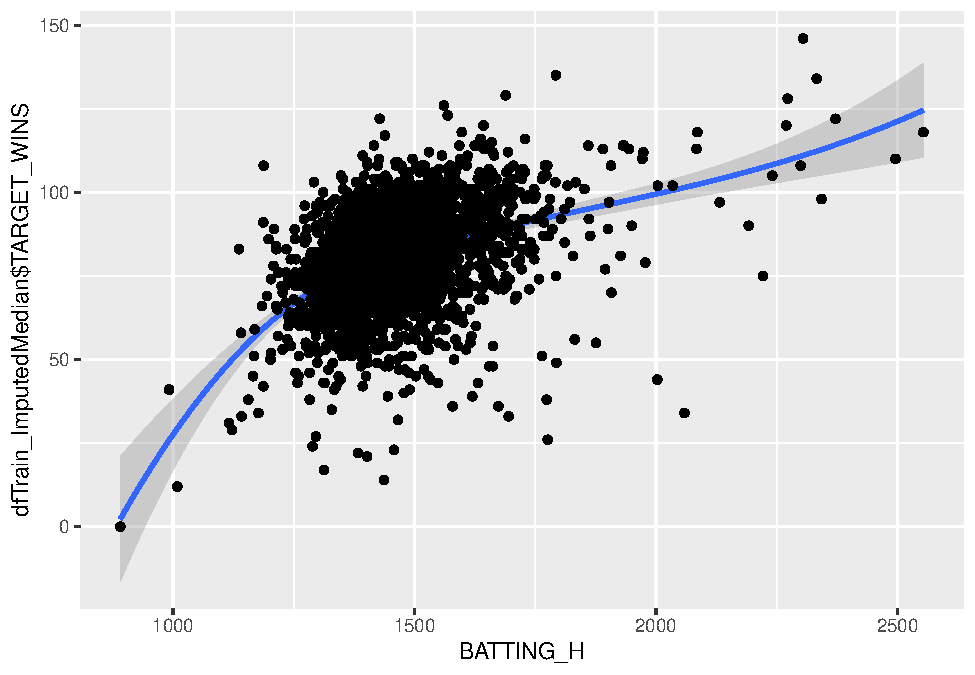
\includegraphics{Baseball5_files/figure-latex/unnamed-chunk-33-3.pdf}

\begin{verbatim}
## 
## Call:
## lm(formula = dfTrain_ImputedMedian$TARGET_WINS ~ dfTrain_ImputedMedian[, 
##     i])
## 
## Residuals:
##     Min      1Q  Median      3Q     Max 
## -71.761  -8.515   0.971   9.783  43.230 
## 
## Coefficients:
##                             Estimate Std. Error t value Pr(>|t|)    
## (Intercept)                17.686332   3.164963   5.588 2.58e-08 ***
## dfTrain_ImputedMedian[, i]  0.042775   0.002136  20.025  < 2e-16 ***
## ---
## Signif. codes:  0 '***' 0.001 '**' 0.01 '*' 0.05 '.' 0.1 ' ' 1
## 
## Residual standard error: 14.31 on 2172 degrees of freedom
## Multiple R-squared:  0.1558, Adjusted R-squared:  0.1555 
## F-statistic:   401 on 1 and 2172 DF,  p-value: < 2.2e-16
\end{verbatim}

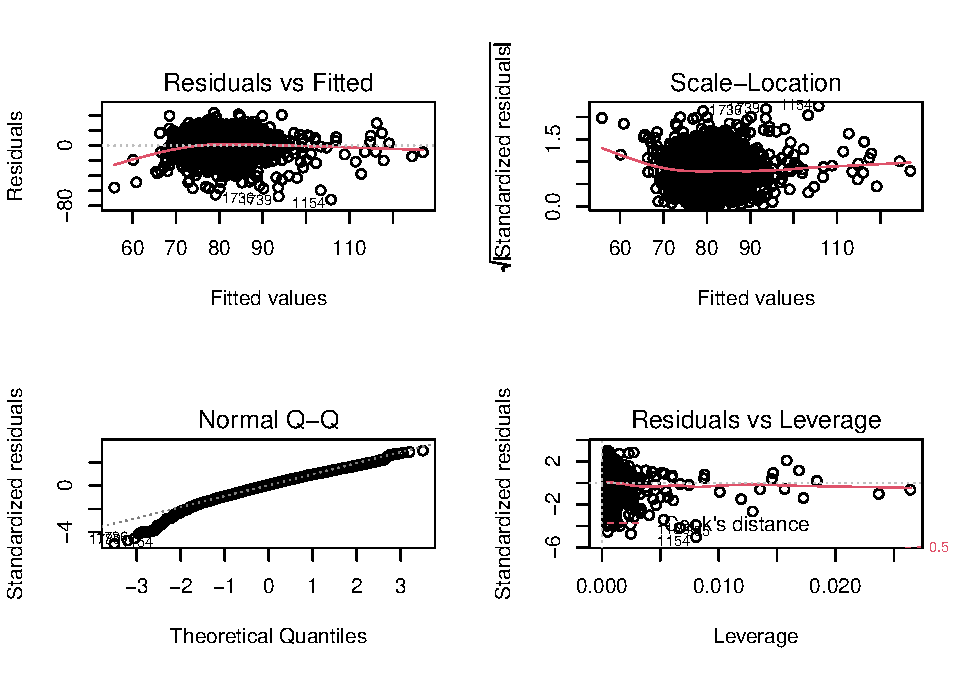
\includegraphics{Baseball5_files/figure-latex/unnamed-chunk-33-4.pdf}

\begin{verbatim}
## NULL
\end{verbatim}

\begin{verbatim}
## Warning: Use of `dfTrain_ImputedMedian$TARGET_WINS` is discouraged. Use
## `TARGET_WINS` instead.

## Warning: Use of `dfTrain_ImputedMedian$TARGET_WINS` is discouraged. Use
## `TARGET_WINS` instead.
\end{verbatim}

\begin{verbatim}
## `geom_smooth()` using formula 'y ~ x'
\end{verbatim}

\includegraphics{Baseball5_files/figure-latex/unnamed-chunk-33-5.pdf}

\begin{verbatim}
## 
## Call:
## lm(formula = dfTrain_ImputedMedian$TARGET_WINS ~ dfTrain_ImputedMedian[, 
##     i])
## 
## Residuals:
##     Min      1Q  Median      3Q     Max 
## -69.863  -9.376   0.670  10.121  57.415 
## 
## Coefficients:
##                             Estimate Std. Error t value Pr(>|t|)    
## (Intercept)                56.346919   1.737969   32.42   <2e-16 ***
## dfTrain_ImputedMedian[, i]  0.100118   0.007005   14.29   <2e-16 ***
## ---
## Signif. codes:  0 '***' 0.001 '**' 0.01 '*' 0.05 '.' 0.1 ' ' 1
## 
## Residual standard error: 14.89 on 2172 degrees of freedom
## Multiple R-squared:  0.08597,    Adjusted R-squared:  0.08555 
## F-statistic: 204.3 on 1 and 2172 DF,  p-value: < 2.2e-16
\end{verbatim}

\includegraphics{Baseball5_files/figure-latex/unnamed-chunk-33-6.pdf}

\begin{verbatim}
## NULL
\end{verbatim}

\begin{verbatim}
## Warning: Use of `dfTrain_ImputedMedian$TARGET_WINS` is discouraged. Use
## `TARGET_WINS` instead.

## Warning: Use of `dfTrain_ImputedMedian$TARGET_WINS` is discouraged. Use
## `TARGET_WINS` instead.
\end{verbatim}

\begin{verbatim}
## `geom_smooth()` using formula 'y ~ x'
\end{verbatim}

\includegraphics{Baseball5_files/figure-latex/unnamed-chunk-33-7.pdf}

\begin{verbatim}
## 
## Call:
## lm(formula = dfTrain_ImputedMedian$TARGET_WINS ~ dfTrain_ImputedMedian[, 
##     i])
## 
## Residuals:
##     Min      1Q  Median      3Q     Max 
## -76.628  -8.980   1.143  10.428  60.940 
## 
## Coefficients:
##                            Estimate Std. Error t value Pr(>|t|)    
## (Intercept)                76.62804    0.72265 106.038  < 2e-16 ***
## dfTrain_ImputedMedian[, i]  0.07596    0.01180   6.439 1.48e-10 ***
## ---
## Signif. codes:  0 '***' 0.001 '**' 0.01 '*' 0.05 '.' 0.1 ' ' 1
## 
## Residual standard error: 15.43 on 2172 degrees of freedom
## Multiple R-squared:  0.01873,    Adjusted R-squared:  0.01828 
## F-statistic: 41.46 on 1 and 2172 DF,  p-value: 1.477e-10
\end{verbatim}

\includegraphics{Baseball5_files/figure-latex/unnamed-chunk-33-8.pdf}

\begin{verbatim}
## NULL
\end{verbatim}

\begin{verbatim}
## Warning: Use of `dfTrain_ImputedMedian$TARGET_WINS` is discouraged. Use
## `TARGET_WINS` instead.

## Warning: Use of `dfTrain_ImputedMedian$TARGET_WINS` is discouraged. Use
## `TARGET_WINS` instead.
\end{verbatim}

\begin{verbatim}
## `geom_smooth()` using formula 'y ~ x'
\end{verbatim}

\includegraphics{Baseball5_files/figure-latex/unnamed-chunk-33-9.pdf}

\begin{verbatim}
## 
## Call:
## lm(formula = dfTrain_ImputedMedian$TARGET_WINS ~ dfTrain_ImputedMedian[, 
##     i])
## 
## Residuals:
##     Min      1Q  Median      3Q     Max 
## -75.596  -9.734   0.553  10.041  68.954 
## 
## Coefficients:
##                             Estimate Std. Error t value Pr(>|t|)    
## (Intercept)                75.595947   0.658670 114.771   <2e-16 ***
## dfTrain_ImputedMedian[, i]  0.050009   0.005527   9.048   <2e-16 ***
## ---
## Signif. codes:  0 '***' 0.001 '**' 0.01 '*' 0.05 '.' 0.1 ' ' 1
## 
## Residual standard error: 15.29 on 2172 degrees of freedom
## Multiple R-squared:  0.03632,    Adjusted R-squared:  0.03588 
## F-statistic: 81.87 on 1 and 2172 DF,  p-value: < 2.2e-16
\end{verbatim}

\includegraphics{Baseball5_files/figure-latex/unnamed-chunk-33-10.pdf}

\begin{verbatim}
## NULL
\end{verbatim}

\begin{verbatim}
## Warning: Use of `dfTrain_ImputedMedian$TARGET_WINS` is discouraged. Use
## `TARGET_WINS` instead.

## Warning: Use of `dfTrain_ImputedMedian$TARGET_WINS` is discouraged. Use
## `TARGET_WINS` instead.
\end{verbatim}

\begin{verbatim}
## `geom_smooth()` using formula 'y ~ x'
\end{verbatim}

\includegraphics{Baseball5_files/figure-latex/unnamed-chunk-33-11.pdf}

\begin{verbatim}
## 
## Call:
## lm(formula = dfTrain_ImputedMedian$TARGET_WINS ~ dfTrain_ImputedMedian[, 
##     i])
## 
## Residuals:
##     Min      1Q  Median      3Q     Max 
## -65.936  -9.554   0.579   9.674  78.185 
## 
## Coefficients:
##                             Estimate Std. Error t value Pr(>|t|)    
## (Intercept)                65.935670   1.370076   48.13   <2e-16 ***
## dfTrain_ImputedMedian[, i]  0.029358   0.002635   11.14   <2e-16 ***
## ---
## Signif. codes:  0 '***' 0.001 '**' 0.01 '*' 0.05 '.' 0.1 ' ' 1
## 
## Residual standard error: 15.15 on 2172 degrees of freedom
## Multiple R-squared:  0.05406,    Adjusted R-squared:  0.05362 
## F-statistic: 124.1 on 1 and 2172 DF,  p-value: < 2.2e-16
\end{verbatim}

\includegraphics{Baseball5_files/figure-latex/unnamed-chunk-33-12.pdf}

\begin{verbatim}
## NULL
\end{verbatim}

\begin{verbatim}
## Warning: Use of `dfTrain_ImputedMedian$TARGET_WINS` is discouraged. Use
## `TARGET_WINS` instead.

## Warning: Use of `dfTrain_ImputedMedian$TARGET_WINS` is discouraged. Use
## `TARGET_WINS` instead.
\end{verbatim}

\begin{verbatim}
## `geom_smooth()` using formula 'y ~ x'
\end{verbatim}

\includegraphics{Baseball5_files/figure-latex/unnamed-chunk-33-13.pdf}

\begin{verbatim}
## 
## Call:
## lm(formula = dfTrain_ImputedMedian$TARGET_WINS ~ dfTrain_ImputedMedian[, 
##     i])
## 
## Residuals:
##     Min      1Q  Median      3Q     Max 
## -82.228  -9.308   0.963  10.609  63.772 
## 
## Coefficients:
##                             Estimate Std. Error t value Pr(>|t|)    
## (Intercept)                82.228036   1.043434   78.81   <2e-16 ***
## dfTrain_ImputedMedian[, i] -0.001990   0.001344   -1.48    0.139    
## ---
## Signif. codes:  0 '***' 0.001 '**' 0.01 '*' 0.05 '.' 0.1 ' ' 1
## 
## Residual standard error: 15.57 on 2172 degrees of freedom
## Multiple R-squared:  0.001008,   Adjusted R-squared:  0.0005482 
## F-statistic: 2.192 on 1 and 2172 DF,  p-value: 0.1389
\end{verbatim}

\includegraphics{Baseball5_files/figure-latex/unnamed-chunk-33-14.pdf}

\begin{verbatim}
## NULL
\end{verbatim}

\begin{verbatim}
## Warning: Use of `dfTrain_ImputedMedian$TARGET_WINS` is discouraged. Use
## `TARGET_WINS` instead.

## Warning: Use of `dfTrain_ImputedMedian$TARGET_WINS` is discouraged. Use
## `TARGET_WINS` instead.
\end{verbatim}

\begin{verbatim}
## `geom_smooth()` using formula 'y ~ x'
\end{verbatim}

\includegraphics{Baseball5_files/figure-latex/unnamed-chunk-33-15.pdf}

\begin{verbatim}
## 
## Call:
## lm(formula = dfTrain_ImputedMedian$TARGET_WINS ~ dfTrain_ImputedMedian[, 
##     i])
## 
## Residuals:
##     Min      1Q  Median      3Q     Max 
## -78.284  -9.080   1.024  10.198  65.160 
## 
## Coefficients:
##                            Estimate Std. Error t value Pr(>|t|)    
## (Intercept)                78.28444    0.57917 135.166  < 2e-16 ***
## dfTrain_ImputedMedian[, i]  0.02048    0.00392   5.226  1.9e-07 ***
## ---
## Signif. codes:  0 '***' 0.001 '**' 0.01 '*' 0.05 '.' 0.1 ' ' 1
## 
## Residual standard error: 15.48 on 2172 degrees of freedom
## Multiple R-squared:  0.01242,    Adjusted R-squared:  0.01196 
## F-statistic: 27.31 on 1 and 2172 DF,  p-value: 1.899e-07
\end{verbatim}

\includegraphics{Baseball5_files/figure-latex/unnamed-chunk-33-16.pdf}

\begin{verbatim}
## NULL
\end{verbatim}

\begin{verbatim}
## Warning: Use of `dfTrain_ImputedMedian$TARGET_WINS` is discouraged. Use
## `TARGET_WINS` instead.

## Warning: Use of `dfTrain_ImputedMedian$TARGET_WINS` is discouraged. Use
## `TARGET_WINS` instead.
\end{verbatim}

\begin{verbatim}
## `geom_smooth()` using formula 'y ~ x'
\end{verbatim}

\includegraphics{Baseball5_files/figure-latex/unnamed-chunk-33-17.pdf}

\begin{verbatim}
## 
## Call:
## lm(formula = dfTrain_ImputedMedian$TARGET_WINS ~ dfTrain_ImputedMedian[, 
##     i])
## 
## Residuals:
##     Min      1Q  Median      3Q     Max 
## -80.071  -9.493   1.233  10.483  65.236 
## 
## Coefficients:
##                            Estimate Std. Error t value Pr(>|t|)    
## (Intercept)                80.07067    0.98260  81.489   <2e-16 ***
## dfTrain_ImputedMedian[, i]  0.01314    0.01750   0.751    0.453    
## ---
## Signif. codes:  0 '***' 0.001 '**' 0.01 '*' 0.05 '.' 0.1 ' ' 1
## 
## Residual standard error: 15.57 on 2172 degrees of freedom
## Multiple R-squared:  0.0002595,  Adjusted R-squared:  -0.0002008 
## F-statistic: 0.5637 on 1 and 2172 DF,  p-value: 0.4528
\end{verbatim}

\includegraphics{Baseball5_files/figure-latex/unnamed-chunk-33-18.pdf}

\begin{verbatim}
## NULL
\end{verbatim}

\begin{verbatim}
## Warning: Use of `dfTrain_ImputedMedian$TARGET_WINS` is discouraged. Use
## `TARGET_WINS` instead.

## Warning: Use of `dfTrain_ImputedMedian$TARGET_WINS` is discouraged. Use
## `TARGET_WINS` instead.
\end{verbatim}

\begin{verbatim}
## `geom_smooth()` using formula 'y ~ x'
\end{verbatim}

\includegraphics{Baseball5_files/figure-latex/unnamed-chunk-33-19.pdf}

\begin{verbatim}
## 
## Call:
## lm(formula = dfTrain_ImputedMedian$TARGET_WINS ~ dfTrain_ImputedMedian[, 
##     i])
## 
## Residuals:
##     Min      1Q  Median      3Q     Max 
## -60.165  -9.462   0.897  10.651  68.914 
## 
## Coefficients:
##                              Estimate Std. Error t value Pr(>|t|)    
## (Intercept)                83.0150688  0.5308401 156.384  < 2e-16 ***
## dfTrain_ImputedMedian[, i] -0.0012543  0.0002309  -5.432  6.2e-08 ***
## ---
## Signif. codes:  0 '***' 0.001 '**' 0.01 '*' 0.05 '.' 0.1 ' ' 1
## 
## Residual standard error: 15.47 on 2172 degrees of freedom
## Multiple R-squared:  0.0134, Adjusted R-squared:  0.01295 
## F-statistic:  29.5 on 1 and 2172 DF,  p-value: 6.205e-08
\end{verbatim}

\includegraphics{Baseball5_files/figure-latex/unnamed-chunk-33-20.pdf}

\begin{verbatim}
## NULL
\end{verbatim}

\begin{verbatim}
## Warning: Use of `dfTrain_ImputedMedian$TARGET_WINS` is discouraged. Use
## `TARGET_WINS` instead.

## Warning: Use of `dfTrain_ImputedMedian$TARGET_WINS` is discouraged. Use
## `TARGET_WINS` instead.
\end{verbatim}

\begin{verbatim}
## `geom_smooth()` using formula 'y ~ x'
\end{verbatim}

\includegraphics{Baseball5_files/figure-latex/unnamed-chunk-33-21.pdf}

\begin{verbatim}
## 
## Call:
## lm(formula = dfTrain_ImputedMedian$TARGET_WINS ~ dfTrain_ImputedMedian[, 
##     i])
## 
## Residuals:
##     Min      1Q  Median      3Q     Max 
## -74.906  -9.846   0.705   9.965  67.942 
## 
## Coefficients:
##                             Estimate Std. Error t value Pr(>|t|)    
## (Intercept)                74.905514   0.682649 109.728   <2e-16 ***
## dfTrain_ImputedMedian[, i]  0.053432   0.005465   9.777   <2e-16 ***
## ---
## Signif. codes:  0 '***' 0.001 '**' 0.01 '*' 0.05 '.' 0.1 ' ' 1
## 
## Residual standard error: 15.25 on 2172 degrees of freedom
## Multiple R-squared:  0.04216,    Adjusted R-squared:  0.04171 
## F-statistic: 95.59 on 1 and 2172 DF,  p-value: < 2.2e-16
\end{verbatim}

\includegraphics{Baseball5_files/figure-latex/unnamed-chunk-33-22.pdf}

\begin{verbatim}
## NULL
\end{verbatim}

\begin{verbatim}
## Warning: Use of `dfTrain_ImputedMedian$TARGET_WINS` is discouraged. Use
## `TARGET_WINS` instead.

## Warning: Use of `dfTrain_ImputedMedian$TARGET_WINS` is discouraged. Use
## `TARGET_WINS` instead.
\end{verbatim}

\begin{verbatim}
## `geom_smooth()` using formula 'y ~ x'
\end{verbatim}

\includegraphics{Baseball5_files/figure-latex/unnamed-chunk-33-23.pdf}

\begin{verbatim}
## 
## Call:
## lm(formula = dfTrain_ImputedMedian$TARGET_WINS ~ dfTrain_ImputedMedian[, 
##     i])
## 
## Residuals:
##     Min      1Q  Median      3Q     Max 
## -74.528  -9.251   0.948  10.415  70.006 
## 
## Coefficients:
##                             Estimate Std. Error t value Pr(>|t|)    
## (Intercept)                74.528116   1.149967  64.809  < 2e-16 ***
## dfTrain_ImputedMedian[, i]  0.011187   0.001975   5.664 1.68e-08 ***
## ---
## Signif. codes:  0 '***' 0.001 '**' 0.01 '*' 0.05 '.' 0.1 ' ' 1
## 
## Residual standard error: 15.46 on 2172 degrees of freedom
## Multiple R-squared:  0.01455,    Adjusted R-squared:  0.0141 
## F-statistic: 32.08 on 1 and 2172 DF,  p-value: 1.678e-08
\end{verbatim}

\includegraphics{Baseball5_files/figure-latex/unnamed-chunk-33-24.pdf}

\begin{verbatim}
## NULL
\end{verbatim}

\begin{verbatim}
## Warning: Use of `dfTrain_ImputedMedian$TARGET_WINS` is discouraged. Use
## `TARGET_WINS` instead.

## Warning: Use of `dfTrain_ImputedMedian$TARGET_WINS` is discouraged. Use
## `TARGET_WINS` instead.
\end{verbatim}

\begin{verbatim}
## `geom_smooth()` using formula 'y ~ x'
\end{verbatim}

\includegraphics{Baseball5_files/figure-latex/unnamed-chunk-33-25.pdf}

\begin{verbatim}
## 
## Call:
## lm(formula = dfTrain_ImputedMedian$TARGET_WINS ~ dfTrain_ImputedMedian[, 
##     i])
## 
## Residuals:
##     Min      1Q  Median      3Q     Max 
## -82.570  -9.402   0.970  10.484  63.430 
## 
## Coefficients:
##                              Estimate Std. Error t value Pr(>|t|)    
## (Intercept)                82.5704787  0.5945630 138.876  < 2e-16 ***
## dfTrain_ImputedMedian[, i] -0.0022085  0.0006023  -3.667 0.000252 ***
## ---
## Signif. codes:  0 '***' 0.001 '**' 0.01 '*' 0.05 '.' 0.1 ' ' 1
## 
## Residual standard error: 15.53 on 2172 degrees of freedom
## Multiple R-squared:  0.006152,   Adjusted R-squared:  0.005695 
## F-statistic: 13.45 on 1 and 2172 DF,  p-value: 0.0002515
\end{verbatim}

\includegraphics{Baseball5_files/figure-latex/unnamed-chunk-33-26.pdf}

\begin{verbatim}
## NULL
\end{verbatim}

\begin{verbatim}
## Warning: Use of `dfTrain_ImputedMedian$TARGET_WINS` is discouraged. Use
## `TARGET_WINS` instead.

## Warning: Use of `dfTrain_ImputedMedian$TARGET_WINS` is discouraged. Use
## `TARGET_WINS` instead.
\end{verbatim}

\begin{verbatim}
## `geom_smooth()` using formula 'y ~ x'
\end{verbatim}

\includegraphics{Baseball5_files/figure-latex/unnamed-chunk-33-27.pdf}

\begin{verbatim}
## 
## Call:
## lm(formula = dfTrain_ImputedMedian$TARGET_WINS ~ dfTrain_ImputedMedian[, 
##     i])
## 
## Residuals:
##     Min      1Q  Median      3Q     Max 
## -61.638  -9.847   0.708  10.050  73.590 
## 
## Coefficients:
##                             Estimate Std. Error t value Pr(>|t|)    
## (Intercept)                83.645750   0.476605 175.503   <2e-16 ***
## dfTrain_ImputedMedian[, i] -0.011815   0.001415  -8.352   <2e-16 ***
## ---
## Signif. codes:  0 '***' 0.001 '**' 0.01 '*' 0.05 '.' 0.1 ' ' 1
## 
## Residual standard error: 15.33 on 2172 degrees of freedom
## Multiple R-squared:  0.03112,    Adjusted R-squared:  0.03067 
## F-statistic: 69.75 on 1 and 2172 DF,  p-value: < 2.2e-16
\end{verbatim}

\includegraphics{Baseball5_files/figure-latex/unnamed-chunk-33-28.pdf}

\begin{verbatim}
## NULL
\end{verbatim}

\begin{verbatim}
## Warning: Use of `dfTrain_ImputedMedian$TARGET_WINS` is discouraged. Use
## `TARGET_WINS` instead.

## Warning: Use of `dfTrain_ImputedMedian$TARGET_WINS` is discouraged. Use
## `TARGET_WINS` instead.
\end{verbatim}

\begin{verbatim}
## `geom_smooth()` using formula 'y ~ x'
\end{verbatim}

\includegraphics{Baseball5_files/figure-latex/unnamed-chunk-33-29.pdf}

\begin{verbatim}
## 
## Call:
## lm(formula = dfTrain_ImputedMedian$TARGET_WINS ~ dfTrain_ImputedMedian[, 
##     i])
## 
## Residuals:
##     Min      1Q  Median      3Q     Max 
## -80.809  -9.322   1.075  10.459  65.191 
## 
## Coefficients:
##                            Estimate Std. Error t value Pr(>|t|)    
## (Intercept)                83.70498    2.23001  37.536   <2e-16 ***
## dfTrain_ImputedMedian[, i] -0.01979    0.01484  -1.334    0.182    
## ---
## Signif. codes:  0 '***' 0.001 '**' 0.01 '*' 0.05 '.' 0.1 ' ' 1
## 
## Residual standard error: 15.57 on 2172 degrees of freedom
## Multiple R-squared:  0.0008182,  Adjusted R-squared:  0.0003582 
## F-statistic: 1.779 on 1 and 2172 DF,  p-value: 0.1825
\end{verbatim}

\includegraphics{Baseball5_files/figure-latex/unnamed-chunk-33-30.pdf}

\begin{verbatim}
## NULL
\end{verbatim}

\begin{Shaded}
\begin{Highlighting}[]
\NormalTok{dfTrain\_ImputedMedian }\OtherTok{\textless{}{-}}\NormalTok{ dfTrain\_ImputedMean\_NoCohort}

\NormalTok{EHExplore\_Correlations\_Scatterplots }\OtherTok{\textless{}{-}} \ControlFlowTok{function}\NormalTok{(df, y, }\AttributeTok{flip=}\ConstantTok{FALSE}\NormalTok{)}
\NormalTok{\{}
\NormalTok{  plot\_list }\OtherTok{\textless{}{-}} \FunctionTok{list}\NormalTok{()}
  
\NormalTok{  df }\OtherTok{\textless{}{-}} \FunctionTok{select\_if}\NormalTok{(df, is.numeric)}
  
  \ControlFlowTok{for}\NormalTok{(i }\ControlFlowTok{in} \DecValTok{1}\SpecialCharTok{:}\FunctionTok{ncol}\NormalTok{(df)) \{}
  
\NormalTok{    ct }\OtherTok{\textless{}{-}} \FunctionTok{cor.test}\NormalTok{(df[,i], df[,y])}
    
\NormalTok{  xText }\OtherTok{\textless{}{-}} \FunctionTok{str\_c}\NormalTok{(}\StringTok{"Correlation: "}\NormalTok{, }\FunctionTok{round}\NormalTok{(ct}\SpecialCharTok{$}\NormalTok{estimate,}\DecValTok{2}\NormalTok{), }\StringTok{"   p value: "}\NormalTok{, }\FunctionTok{round}\NormalTok{(ct}\SpecialCharTok{$}\NormalTok{p.value,}\DecValTok{2}\NormalTok{))}
  
\NormalTok{  x1 }\OtherTok{=}\NormalTok{ df[[i]]}
\NormalTok{  y1 }\OtherTok{=}\NormalTok{y}
  
  \ControlFlowTok{if}\NormalTok{(flip)}
\NormalTok{  \{}
\NormalTok{    x1}\OtherTok{=}\NormalTok{y}
\NormalTok{    y1}\OtherTok{=}\NormalTok{df[[i]]}
\NormalTok{  \}}
  
\NormalTok{    p }\OtherTok{\textless{}{-}} \FunctionTok{ggplot}\NormalTok{(df, }\FunctionTok{aes\_string}\NormalTok{(x1, y1)) }\SpecialCharTok{+}
  \FunctionTok{geom\_point}\NormalTok{(}\AttributeTok{fill=}\StringTok{"navy"}\NormalTok{, }\AttributeTok{color=}\StringTok{"white"}\NormalTok{) }\SpecialCharTok{+}
  \FunctionTok{geom\_smooth}\NormalTok{(}\AttributeTok{method =} \StringTok{"loess"}\NormalTok{, }\AttributeTok{color=}\StringTok{"red"}\NormalTok{, }\AttributeTok{fill=}\StringTok{"lightcoral"}\NormalTok{) }\SpecialCharTok{+}
  \FunctionTok{ylab}\NormalTok{(y) }\SpecialCharTok{+}
    \FunctionTok{xlab}\NormalTok{(xText) }\SpecialCharTok{+}
    \FunctionTok{theme}\NormalTok{(}\AttributeTok{title =} \FunctionTok{element\_text}\NormalTok{(}\AttributeTok{size=}\DecValTok{9}\NormalTok{), }\AttributeTok{axis.title.x =} \FunctionTok{element\_text}\NormalTok{(}\AttributeTok{size =} \DecValTok{8}\NormalTok{), }\AttributeTok{axis.title.y =} \FunctionTok{element\_text}\NormalTok{(}\AttributeTok{size =} \DecValTok{9}\NormalTok{), }\AttributeTok{axis.text.x =} \FunctionTok{element\_text}\NormalTok{(}\AttributeTok{size =} \DecValTok{8}\NormalTok{), }\AttributeTok{axis.ticks.x =} \FunctionTok{element\_blank}\NormalTok{(), }\AttributeTok{panel.grid.major.x =} \FunctionTok{element\_blank}\NormalTok{(), }\AttributeTok{panel.grid.minor.x=}\FunctionTok{element\_blank}\NormalTok{(), }\AttributeTok{panel.grid.minor.y=}\FunctionTok{element\_blank}\NormalTok{(), }\AttributeTok{panel.grid.major.y=}\FunctionTok{element\_line}\NormalTok{(}\AttributeTok{color=}\StringTok{"gray"}\NormalTok{), }\AttributeTok{panel.background =} \FunctionTok{element\_rect}\NormalTok{(}\AttributeTok{fill =} \StringTok{"slategray2"}\NormalTok{, }\AttributeTok{color=}\StringTok{"darkslategray"}\NormalTok{)) }\SpecialCharTok{+}
  \FunctionTok{ggtitle}\NormalTok{(}\FunctionTok{colnames}\NormalTok{(df)[i])}

\NormalTok{  p }\OtherTok{\textless{}{-}} \FunctionTok{eval}\NormalTok{(}\FunctionTok{substitute}\NormalTok{(p, }\FunctionTok{list}\NormalTok{(}\AttributeTok{i=}\NormalTok{i)))}
\NormalTok{  plot\_list[[i]] }\OtherTok{\textless{}{-}}\NormalTok{ p }
    
\NormalTok{\}}
  \FunctionTok{return}\NormalTok{(plot\_list)}
\NormalTok{\}}

\NormalTok{z4 }\OtherTok{\textless{}{-}} \FunctionTok{EHExplore\_Correlations\_Scatterplots}\NormalTok{(dfTrain\_ImputedMedian, }\StringTok{"TARGET\_WINS"}\NormalTok{)}

\FunctionTok{grid.arrange}\NormalTok{(}\AttributeTok{grobs=}\NormalTok{z4[}\FunctionTok{c}\NormalTok{(}\DecValTok{2}\SpecialCharTok{:}\DecValTok{11}\NormalTok{)],  }\AttributeTok{ncol=}\DecValTok{3}\NormalTok{, }\AttributeTok{nrow=}\DecValTok{5}\NormalTok{)}
\end{Highlighting}
\end{Shaded}

\begin{verbatim}
## `geom_smooth()` using formula 'y ~ x'
## `geom_smooth()` using formula 'y ~ x'
## `geom_smooth()` using formula 'y ~ x'
## `geom_smooth()` using formula 'y ~ x'
## `geom_smooth()` using formula 'y ~ x'
## `geom_smooth()` using formula 'y ~ x'
## `geom_smooth()` using formula 'y ~ x'
## `geom_smooth()` using formula 'y ~ x'
## `geom_smooth()` using formula 'y ~ x'
## `geom_smooth()` using formula 'y ~ x'
\end{verbatim}

\includegraphics{Baseball5_files/figure-latex/unnamed-chunk-34-1.pdf}

\begin{Shaded}
\begin{Highlighting}[]
\CommentTok{\#grid.arrange(grobs=z4[c(11:16)],  ncol=3, nrow=6)}
\end{Highlighting}
\end{Shaded}

\begin{Shaded}
\begin{Highlighting}[]
\NormalTok{EHExplore\_IntegratePlotLists }\OtherTok{\textless{}{-}}\ControlFlowTok{function}\NormalTok{(list1, list2, list3)}
\NormalTok{\{  }
\NormalTok{zz2 }\OtherTok{\textless{}{-}} \FunctionTok{list}\NormalTok{()}

\ControlFlowTok{for}\NormalTok{(i }\ControlFlowTok{in} \DecValTok{1}\SpecialCharTok{:}\FunctionTok{length}\NormalTok{(list1)) \{}
\NormalTok{zz2[i}\SpecialCharTok{*}\DecValTok{3{-}2}\NormalTok{] }\OtherTok{\textless{}{-}}\NormalTok{ list1[i]}
\NormalTok{zz2[i}\SpecialCharTok{*}\DecValTok{3{-}1}\NormalTok{] }\OtherTok{\textless{}{-}}\NormalTok{ list2[i]}
\NormalTok{zz2[i}\SpecialCharTok{*}\DecValTok{3}\NormalTok{] }\OtherTok{\textless{}{-}}\NormalTok{ list3[i]}
\NormalTok{\}}
\FunctionTok{return}\NormalTok{(zz2)}
\NormalTok{\}}



\NormalTok{zz1 }\OtherTok{\textless{}{-}} \FunctionTok{list}\NormalTok{()}

\ControlFlowTok{for}\NormalTok{(i }\ControlFlowTok{in} \DecValTok{1}\SpecialCharTok{:}\FunctionTok{length}\NormalTok{(z)) \{}
\NormalTok{zz1[i}\SpecialCharTok{*}\DecValTok{3{-}2}\NormalTok{] }\OtherTok{\textless{}{-}}\NormalTok{ z[i]}
\NormalTok{zz1[i}\SpecialCharTok{*}\DecValTok{3{-}1}\NormalTok{] }\OtherTok{\textless{}{-}}\NormalTok{ z6[i]}
\NormalTok{zz1[i}\SpecialCharTok{*}\DecValTok{3}\NormalTok{] }\OtherTok{\textless{}{-}}\NormalTok{ z4[i]}
\NormalTok{\}}

\FunctionTok{grid.arrange}\NormalTok{(}\AttributeTok{grobs=}\NormalTok{zz1[}\FunctionTok{c}\NormalTok{(}\DecValTok{1}\SpecialCharTok{:}\DecValTok{24}\NormalTok{)],  }\AttributeTok{ncol=}\DecValTok{3}\NormalTok{, }\AttributeTok{nrow=}\DecValTok{8}\NormalTok{)}
\end{Highlighting}
\end{Shaded}

\begin{verbatim}
## `geom_smooth()` using formula 'y ~ x'
## `geom_smooth()` using formula 'y ~ x'
## `geom_smooth()` using formula 'y ~ x'
## `geom_smooth()` using formula 'y ~ x'
## `geom_smooth()` using formula 'y ~ x'
## `geom_smooth()` using formula 'y ~ x'
## `geom_smooth()` using formula 'y ~ x'
## `geom_smooth()` using formula 'y ~ x'
\end{verbatim}

\includegraphics{Baseball5_files/figure-latex/unnamed-chunk-35-1.pdf}

\begin{Shaded}
\begin{Highlighting}[]
\FunctionTok{grid.arrange}\NormalTok{(}\AttributeTok{grobs=}\NormalTok{zz1[}\FunctionTok{c}\NormalTok{(}\DecValTok{25}\SpecialCharTok{:}\DecValTok{48}\NormalTok{)],  }\AttributeTok{ncol=}\DecValTok{3}\NormalTok{, }\AttributeTok{nrow=}\DecValTok{8}\NormalTok{)}
\end{Highlighting}
\end{Shaded}

\begin{verbatim}
## `geom_smooth()` using formula 'y ~ x'
## `geom_smooth()` using formula 'y ~ x'
## `geom_smooth()` using formula 'y ~ x'
## `geom_smooth()` using formula 'y ~ x'
## `geom_smooth()` using formula 'y ~ x'
## `geom_smooth()` using formula 'y ~ x'
## `geom_smooth()` using formula 'y ~ x'
## `geom_smooth()` using formula 'y ~ x'
\end{verbatim}

\includegraphics{Baseball5_files/figure-latex/unnamed-chunk-35-2.pdf}

\begin{Shaded}
\begin{Highlighting}[]
\CommentTok{\#grid.arrange(grobs=zz1[c(25:36)],  ncol=3, nrow=4)}
\CommentTok{\#grid.arrange(grobs=zz1[c(37:48)],  ncol=3, nrow=4)}
\end{Highlighting}
\end{Shaded}

Trying a transformation on team fielding error. it improves it to some
degree.

\begin{Shaded}
\begin{Highlighting}[]
\NormalTok{dfTrain\_ImputedMedian2 }\OtherTok{\textless{}{-}}\NormalTok{ dfTrain\_ImputedMedian }\SpecialCharTok{\%\textgreater{}\%}
  \FunctionTok{mutate}\NormalTok{(}\AttributeTok{sq =}\NormalTok{ FIELDING\_E}\SpecialCharTok{\^{}}\DecValTok{2}\NormalTok{)}

\FunctionTok{summary}\NormalTok{(}\FunctionTok{lm}\NormalTok{(TARGET\_WINS }\SpecialCharTok{\textasciitilde{}}\NormalTok{ FIELDING\_E, dfTrain\_ImputedMedian2))}
\end{Highlighting}
\end{Shaded}

\begin{verbatim}
## 
## Call:
## lm(formula = TARGET_WINS ~ FIELDING_E, data = dfTrain_ImputedMedian2)
## 
## Residuals:
##     Min      1Q  Median      3Q     Max 
## -61.638  -9.847   0.708  10.050  73.590 
## 
## Coefficients:
##              Estimate Std. Error t value Pr(>|t|)    
## (Intercept) 83.645750   0.476605 175.503   <2e-16 ***
## FIELDING_E  -0.011815   0.001415  -8.352   <2e-16 ***
## ---
## Signif. codes:  0 '***' 0.001 '**' 0.01 '*' 0.05 '.' 0.1 ' ' 1
## 
## Residual standard error: 15.33 on 2172 degrees of freedom
## Multiple R-squared:  0.03112,    Adjusted R-squared:  0.03067 
## F-statistic: 69.75 on 1 and 2172 DF,  p-value: < 2.2e-16
\end{verbatim}

\begin{Shaded}
\begin{Highlighting}[]
\FunctionTok{summary}\NormalTok{(}\FunctionTok{lm}\NormalTok{(TARGET\_WINS }\SpecialCharTok{\textasciitilde{}}\NormalTok{ FIELDING\_E }\SpecialCharTok{+}\NormalTok{ sq, dfTrain\_ImputedMedian2))}
\end{Highlighting}
\end{Shaded}

\begin{verbatim}
## 
## Call:
## lm(formula = TARGET_WINS ~ FIELDING_E + sq, data = dfTrain_ImputedMedian2)
## 
## Residuals:
##     Min      1Q  Median      3Q     Max 
## -63.981  -9.787   0.647  10.285  72.647 
## 
## Coefficients:
##               Estimate Std. Error t value Pr(>|t|)    
## (Intercept)  7.985e+01  7.178e-01 111.246  < 2e-16 ***
## FIELDING_E   1.386e-02  3.924e-03   3.533 0.000419 ***
## sq          -2.177e-05  3.108e-06  -7.005 3.29e-12 ***
## ---
## Signif. codes:  0 '***' 0.001 '**' 0.01 '*' 0.05 '.' 0.1 ' ' 1
## 
## Residual standard error: 15.17 on 2171 degrees of freedom
## Multiple R-squared:  0.05253,    Adjusted R-squared:  0.05165 
## F-statistic: 60.18 on 2 and 2171 DF,  p-value: < 2.2e-16
\end{verbatim}

\hypertarget{regression}{%
\subsubsection{Regression}\label{regression}}

\begin{Shaded}
\begin{Highlighting}[]
\CommentTok{\#Two mods made {-} team pitching has the square temr and intreaction between hits and dp}

\FunctionTok{par}\NormalTok{(}\AttributeTok{mfcol=}\FunctionTok{c}\NormalTok{(}\DecValTok{2}\NormalTok{,}\DecValTok{2}\NormalTok{))}
\NormalTok{mod\_2 }\OtherTok{\textless{}{-}} \FunctionTok{lm}\NormalTok{(TARGET\_WINS }\SpecialCharTok{\textasciitilde{}}\NormalTok{ ., }\AttributeTok{data =}\NormalTok{ dfTrain\_ImputedMedian)}
\FunctionTok{summary}\NormalTok{(mod\_2)}
\end{Highlighting}
\end{Shaded}

\begin{verbatim}
## 
## Call:
## lm(formula = TARGET_WINS ~ ., data = dfTrain_ImputedMedian)
## 
## Residuals:
##     Min      1Q  Median      3Q     Max 
## -50.264  -8.466   0.163   8.273  58.924 
## 
## Coefficients:
##               Estimate Std. Error t value Pr(>|t|)    
## (Intercept) 23.9560970  5.4876280   4.365 1.33e-05 ***
## INDEX       -0.0004771  0.0003788  -1.259 0.207988    
## BATTING_H    0.0482928  0.0037112  13.013  < 2e-16 ***
## BATTING_2B  -0.0232530  0.0092311  -2.519 0.011841 *  
## BATTING_3B   0.0595670  0.0169134   3.522 0.000437 ***
## BATTING_HR   0.0655424  0.0272468   2.406 0.016234 *  
## BATTING_BB   0.0084691  0.0057882   1.463 0.143567    
## BATTING_SO  -0.0100510  0.0025721  -3.908 9.61e-05 ***
## BASERUN_SB   0.0254437  0.0044746   5.686 1.47e-08 ***
## BASERUN_CS   0.0006521  0.0161429   0.040 0.967780    
## PITCHING_H  -0.0009865  0.0003651  -2.702 0.006949 ** 
## PITCHING_HR  0.0116273  0.0240289   0.484 0.628514    
## PITCHING_BB  0.0014808  0.0040999   0.361 0.718000    
## PITCHING_SO  0.0028141  0.0009069   3.103 0.001941 ** 
## FIELDING_E  -0.0186779  0.0024906  -7.499 9.31e-14 ***
## FIELDING_DP -0.1091373  0.0136377  -8.003 1.97e-15 ***
## ---
## Signif. codes:  0 '***' 0.001 '**' 0.01 '*' 0.05 '.' 0.1 ' ' 1
## 
## Residual standard error: 12.86 on 2158 degrees of freedom
## Multiple R-squared:  0.3226, Adjusted R-squared:  0.3179 
## F-statistic:  68.5 on 15 and 2158 DF,  p-value: < 2.2e-16
\end{verbatim}

\begin{Shaded}
\begin{Highlighting}[]
\FunctionTok{plot}\NormalTok{(mod\_2)}
\end{Highlighting}
\end{Shaded}

\includegraphics{Baseball5_files/figure-latex/unnamed-chunk-37-1.pdf}

\begin{Shaded}
\begin{Highlighting}[]
\FunctionTok{library}\NormalTok{(MASS)}
\end{Highlighting}
\end{Shaded}

\begin{verbatim}
## Warning: package 'MASS' was built under R version 4.0.5
\end{verbatim}

\begin{verbatim}
## 
## Attaching package: 'MASS'
\end{verbatim}

\begin{verbatim}
## The following object is masked from 'package:patchwork':
## 
##     area
\end{verbatim}

\begin{verbatim}
## The following object is masked from 'package:dplyr':
## 
##     select
\end{verbatim}

\begin{Shaded}
\begin{Highlighting}[]
\NormalTok{step1 }\OtherTok{\textless{}{-}} \FunctionTok{stepAIC}\NormalTok{(mod\_2, }\AttributeTok{trace=}\ConstantTok{FALSE}\NormalTok{)}
\FunctionTok{summary}\NormalTok{(step1)}
\end{Highlighting}
\end{Shaded}

\begin{verbatim}
## 
## Call:
## lm(formula = TARGET_WINS ~ BATTING_H + BATTING_2B + BATTING_3B + 
##     BATTING_HR + BATTING_BB + BATTING_SO + BASERUN_SB + PITCHING_H + 
##     PITCHING_SO + FIELDING_E + FIELDING_DP, data = dfTrain_ImputedMedian)
## 
## Residuals:
##     Min      1Q  Median      3Q     Max 
## -50.153  -8.411   0.176   8.307  58.465 
## 
## Coefficients:
##               Estimate Std. Error t value Pr(>|t|)    
## (Intercept) 22.6861348  5.2806294   4.296 1.82e-05 ***
## BATTING_H    0.0486089  0.0036841  13.194  < 2e-16 ***
## BATTING_2B  -0.0233877  0.0092203  -2.537 0.011265 *  
## BATTING_3B   0.0602198  0.0166990   3.606 0.000318 ***
## BATTING_HR   0.0770786  0.0097715   7.888 4.83e-15 ***
## BATTING_BB   0.0104799  0.0033563   3.122 0.001817 ** 
## BATTING_SO  -0.0104007  0.0024834  -4.188 2.93e-05 ***
## BASERUN_SB   0.0253857  0.0042813   5.929 3.53e-09 ***
## PITCHING_H  -0.0008928  0.0003178  -2.809 0.005008 ** 
## PITCHING_SO  0.0030690  0.0006625   4.633 3.82e-06 ***
## FIELDING_E  -0.0184139  0.0024107  -7.639 3.28e-14 ***
## FIELDING_DP -0.1095211  0.0136173  -8.043 1.43e-15 ***
## ---
## Signif. codes:  0 '***' 0.001 '**' 0.01 '*' 0.05 '.' 0.1 ' ' 1
## 
## Residual standard error: 12.86 on 2162 degrees of freedom
## Multiple R-squared:  0.3218, Adjusted R-squared:  0.3184 
## F-statistic: 93.27 on 11 and 2162 DF,  p-value: < 2.2e-16
\end{verbatim}

Understanding the role of double plays - remove the influence of hits:

\begin{Shaded}
\begin{Highlighting}[]
\FunctionTok{ggplot}\NormalTok{(dfTrain\_ImputedMedian, }\FunctionTok{aes}\NormalTok{(FIELDING\_DP, PITCHING\_H)) }\SpecialCharTok{+}
  \FunctionTok{geom\_point}\NormalTok{()}
\end{Highlighting}
\end{Shaded}

\includegraphics{Baseball5_files/figure-latex/unnamed-chunk-38-1.pdf}

\begin{Shaded}
\begin{Highlighting}[]
\FunctionTok{ggplot}\NormalTok{(dfTrain, }\FunctionTok{aes}\NormalTok{(FIELDING\_DP, PITCHING\_H)) }\SpecialCharTok{+}
  \FunctionTok{geom\_point}\NormalTok{()}
\end{Highlighting}
\end{Shaded}

\begin{verbatim}
## Warning: Removed 286 rows containing missing values (geom_point).
\end{verbatim}

\includegraphics{Baseball5_files/figure-latex/unnamed-chunk-38-2.pdf}

\begin{Shaded}
\begin{Highlighting}[]
\FunctionTok{cor}\NormalTok{(dfTrain\_ImputedMedian}\SpecialCharTok{$}\NormalTok{FIELDING\_DP, dfTrain\_ImputedMedian}\SpecialCharTok{$}\NormalTok{PITCHING\_H)}
\end{Highlighting}
\end{Shaded}

\begin{verbatim}
## [1] -0.08895731
\end{verbatim}

\begin{Shaded}
\begin{Highlighting}[]
\FunctionTok{summary}\NormalTok{(}\FunctionTok{lm}\NormalTok{(TARGET\_WINS }\SpecialCharTok{\textasciitilde{}}\NormalTok{ FIELDING\_DP }\SpecialCharTok{+}\NormalTok{ PITCHING\_H, dfTrain))}
\end{Highlighting}
\end{Shaded}

\begin{verbatim}
## 
## Call:
## lm(formula = TARGET_WINS ~ FIELDING_DP + PITCHING_H, data = dfTrain)
## 
## Residuals:
##     Min      1Q  Median      3Q     Max 
## -66.999  -9.102   0.739  10.013  43.146 
## 
## Coefficients:
##               Estimate Std. Error t value Pr(>|t|)    
## (Intercept) 75.0829610  2.4592867  30.530  < 2e-16 ***
## FIELDING_DP -0.0045343  0.0121655  -0.373    0.709    
## PITCHING_H   0.0041845  0.0008319   5.030 5.34e-07 ***
## ---
## Signif. codes:  0 '***' 0.001 '**' 0.01 '*' 0.05 '.' 0.1 ' ' 1
## 
## Residual standard error: 13.85 on 1987 degrees of freedom
##   (286 observations deleted due to missingness)
## Multiple R-squared:  0.01377,    Adjusted R-squared:  0.01278 
## F-statistic: 13.87 on 2 and 1987 DF,  p-value: 1.038e-06
\end{verbatim}

\begin{Shaded}
\begin{Highlighting}[]
\FunctionTok{summary}\NormalTok{(}\FunctionTok{lm}\NormalTok{(TARGET\_WINS }\SpecialCharTok{\textasciitilde{}}\NormalTok{ FIELDING\_DP }\SpecialCharTok{+}\NormalTok{ PITCHING\_H, dfTrain\_ImputedMedian))}
\end{Highlighting}
\end{Shaded}

\begin{verbatim}
## 
## Call:
## lm(formula = TARGET_WINS ~ FIELDING_DP + PITCHING_H, data = dfTrain_ImputedMedian)
## 
## Residuals:
##     Min      1Q  Median      3Q     Max 
## -60.237  -9.564   0.855  10.359  68.964 
## 
## Coefficients:
##               Estimate Std. Error t value Pr(>|t|)    
## (Intercept) 87.1139149  2.2975487  37.916  < 2e-16 ***
## FIELDING_DP -0.0271240  0.0147930  -1.834   0.0669 .  
## PITCHING_H  -0.0012921  0.0002317  -5.576 2.76e-08 ***
## ---
## Signif. codes:  0 '***' 0.001 '**' 0.01 '*' 0.05 '.' 0.1 ' ' 1
## 
## Residual standard error: 15.46 on 2171 degrees of freedom
## Multiple R-squared:  0.01493,    Adjusted R-squared:  0.01402 
## F-statistic: 16.45 on 2 and 2171 DF,  p-value: 8.127e-08
\end{verbatim}

\begin{Shaded}
\begin{Highlighting}[]
\FunctionTok{summary}\NormalTok{(}\FunctionTok{lm}\NormalTok{(TARGET\_WINS }\SpecialCharTok{\textasciitilde{}}\NormalTok{ FIELDING\_DP}\SpecialCharTok{*}\NormalTok{PITCHING\_H, dfTrain))}
\end{Highlighting}
\end{Shaded}

\begin{verbatim}
## 
## Call:
## lm(formula = TARGET_WINS ~ FIELDING_DP * PITCHING_H, data = dfTrain)
## 
## Residuals:
##     Min      1Q  Median      3Q     Max 
## -69.126  -9.261   1.004   9.713  47.202 
## 
## Coefficients:
##                          Estimate Std. Error t value Pr(>|t|)    
## (Intercept)             1.023e+02  5.724e+00  17.872  < 2e-16 ***
## FIELDING_DP            -2.549e-01  4.914e-02  -5.188 2.35e-07 ***
## PITCHING_H             -1.244e-02  3.269e-03  -3.806 0.000145 ***
## FIELDING_DP:PITCHING_H  1.561e-04  2.970e-05   5.257 1.62e-07 ***
## ---
## Signif. codes:  0 '***' 0.001 '**' 0.01 '*' 0.05 '.' 0.1 ' ' 1
## 
## Residual standard error: 13.76 on 1986 degrees of freedom
##   (286 observations deleted due to missingness)
## Multiple R-squared:  0.02731,    Adjusted R-squared:  0.02584 
## F-statistic: 18.59 on 3 and 1986 DF,  p-value: 6.864e-12
\end{verbatim}

\begin{Shaded}
\begin{Highlighting}[]
\FunctionTok{summary}\NormalTok{(}\FunctionTok{lm}\NormalTok{(TARGET\_WINS }\SpecialCharTok{\textasciitilde{}}\NormalTok{ FIELDING\_DP}\SpecialCharTok{*}\NormalTok{PITCHING\_H, dfTrain\_ImputedMedian))}
\end{Highlighting}
\end{Shaded}

\begin{verbatim}
## 
## Call:
## lm(formula = TARGET_WINS ~ FIELDING_DP * PITCHING_H, data = dfTrain_ImputedMedian)
## 
## Residuals:
##     Min      1Q  Median      3Q     Max 
## -60.162  -9.515   0.820  10.312  69.257 
## 
## Coefficients:
##                          Estimate Std. Error t value Pr(>|t|)    
## (Intercept)             7.833e+01  5.757e+00  13.607   <2e-16 ***
## FIELDING_DP             3.302e-02  3.906e-02   0.845   0.3981    
## PITCHING_H              3.513e-03  2.898e-03   1.212   0.2256    
## FIELDING_DP:PITCHING_H -3.328e-05  2.001e-05  -1.663   0.0964 .  
## ---
## Signif. codes:  0 '***' 0.001 '**' 0.01 '*' 0.05 '.' 0.1 ' ' 1
## 
## Residual standard error: 15.46 on 2170 degrees of freedom
## Multiple R-squared:  0.01618,    Adjusted R-squared:  0.01482 
## F-statistic:  11.9 on 3 and 2170 DF,  p-value: 9.984e-08
\end{verbatim}

The interaction temr makes a difference.

Taking a log of Pitching\_H:

\begin{Shaded}
\begin{Highlighting}[]
\FunctionTok{ggplot}\NormalTok{(dfTrain\_ImputedMedian, }\FunctionTok{aes}\NormalTok{(dfTrain\_ImputedMedian}\SpecialCharTok{$}\NormalTok{PITCHING\_H)) }\SpecialCharTok{+}
  \FunctionTok{geom\_histogram}\NormalTok{(}\AttributeTok{bins=}\DecValTok{100}\NormalTok{)}
\end{Highlighting}
\end{Shaded}

\begin{verbatim}
## Warning: Use of `dfTrain_ImputedMedian$PITCHING_H` is discouraged. Use
## `PITCHING_H` instead.
\end{verbatim}

\includegraphics{Baseball5_files/figure-latex/unnamed-chunk-39-1.pdf}

\begin{Shaded}
\begin{Highlighting}[]
\NormalTok{dfTrain\_ImputedMedian5 }\OtherTok{\textless{}{-}}\NormalTok{ dfTrain\_ImputedMedian2 }\SpecialCharTok{\%\textgreater{}\%}
  \FunctionTok{mutate}\NormalTok{(}\AttributeTok{logPitch\_h =}\NormalTok{ PITCHING\_H}\SpecialCharTok{\^{}}\DecValTok{2}\NormalTok{)}

\FunctionTok{ggplot}\NormalTok{(dfTrain\_ImputedMedian5, }\FunctionTok{aes}\NormalTok{(logPitch\_h, TARGET\_WINS)) }\SpecialCharTok{+}
          \FunctionTok{stat\_smooth}\NormalTok{(}\AttributeTok{method=}\NormalTok{loess) }\SpecialCharTok{+}
          \FunctionTok{geom\_point}\NormalTok{()}
\end{Highlighting}
\end{Shaded}

\begin{verbatim}
## `geom_smooth()` using formula 'y ~ x'
\end{verbatim}

\includegraphics{Baseball5_files/figure-latex/unnamed-chunk-39-2.pdf}

\begin{Shaded}
\begin{Highlighting}[]
\NormalTok{m }\OtherTok{\textless{}{-}} \FunctionTok{lm}\NormalTok{(TARGET\_WINS }\SpecialCharTok{\textasciitilde{}}\NormalTok{ PITCHING\_H }\SpecialCharTok{+}\NormalTok{ logPitch\_h, dfTrain\_ImputedMedian5)}
\FunctionTok{summary}\NormalTok{(m)}
\end{Highlighting}
\end{Shaded}

\begin{verbatim}
## 
## Call:
## lm(formula = TARGET_WINS ~ PITCHING_H + logPitch_h, data = dfTrain_ImputedMedian5)
## 
## Residuals:
##     Min      1Q  Median      3Q     Max 
## -63.631  -9.694   1.045  10.242  64.174 
## 
## Coefficients:
##               Estimate Std. Error t value Pr(>|t|)    
## (Intercept)  7.944e+01  9.013e-01  88.133  < 2e-16 ***
## PITCHING_H   1.126e-03  5.376e-04   2.094   0.0364 *  
## logPitch_h  -1.313e-07  2.682e-08  -4.897 1.05e-06 ***
## ---
## Signif. codes:  0 '***' 0.001 '**' 0.01 '*' 0.05 '.' 0.1 ' ' 1
## 
## Residual standard error: 15.39 on 2171 degrees of freedom
## Multiple R-squared:  0.02418,    Adjusted R-squared:  0.02328 
## F-statistic:  26.9 on 2 and 2171 DF,  p-value: 2.895e-12
\end{verbatim}

\begin{Shaded}
\begin{Highlighting}[]
\FunctionTok{plot}\NormalTok{(m)}
\end{Highlighting}
\end{Shaded}

\includegraphics{Baseball5_files/figure-latex/unnamed-chunk-39-3.pdf}
\includegraphics{Baseball5_files/figure-latex/unnamed-chunk-39-4.pdf}
\includegraphics{Baseball5_files/figure-latex/unnamed-chunk-39-5.pdf}
\includegraphics{Baseball5_files/figure-latex/unnamed-chunk-39-6.pdf}

A closer look at Pitching\_h. Taking out th outliers.

\begin{Shaded}
\begin{Highlighting}[]
\NormalTok{dfTrain\_ImputedMedian6 }\OtherTok{\textless{}{-}}\NormalTok{ dfTrain\_ImputedMedian5 }\SpecialCharTok{\%\textgreater{}\%}
\NormalTok{  dplyr}\SpecialCharTok{::}\FunctionTok{filter}\NormalTok{(PITCHING\_H }\SpecialCharTok{\textless{}=} \DecValTok{1500}\NormalTok{)}

\NormalTok{dfTrain\_ImputedMedian7 }\OtherTok{\textless{}{-}}\NormalTok{ dfTrain\_ImputedMedian5 }\SpecialCharTok{\%\textgreater{}\%}
\NormalTok{  dplyr}\SpecialCharTok{::}\FunctionTok{filter}\NormalTok{(PITCHING\_H }\SpecialCharTok{\textgreater{}} \DecValTok{2000}\NormalTok{)}

\FunctionTok{ggplot}\NormalTok{(dfTrain\_ImputedMedian6, }\FunctionTok{aes}\NormalTok{(PITCHING\_H, TARGET\_WINS)) }\SpecialCharTok{+}
          \FunctionTok{stat\_smooth}\NormalTok{(}\AttributeTok{method=}\NormalTok{loess) }\SpecialCharTok{+}
          \FunctionTok{geom\_point}\NormalTok{()}
\end{Highlighting}
\end{Shaded}

\begin{verbatim}
## `geom_smooth()` using formula 'y ~ x'
\end{verbatim}

\includegraphics{Baseball5_files/figure-latex/unnamed-chunk-40-1.pdf}

\begin{Shaded}
\begin{Highlighting}[]
\NormalTok{m }\OtherTok{\textless{}{-}} \FunctionTok{lm}\NormalTok{(TARGET\_WINS }\SpecialCharTok{\textasciitilde{}}\NormalTok{ PITCHING\_H, dfTrain\_ImputedMedian6)}
\FunctionTok{summary}\NormalTok{(m)}
\end{Highlighting}
\end{Shaded}

\begin{verbatim}
## 
## Call:
## lm(formula = TARGET_WINS ~ PITCHING_H, data = dfTrain_ImputedMedian6)
## 
## Residuals:
##     Min      1Q  Median      3Q     Max 
## -60.864  -8.396   0.413   8.870  30.267 
## 
## Coefficients:
##             Estimate Std. Error t value Pr(>|t|)    
## (Intercept)  8.26774    8.46728   0.976    0.329    
## PITCHING_H   0.04990    0.00602   8.289 3.78e-16 ***
## ---
## Signif. codes:  0 '***' 0.001 '**' 0.01 '*' 0.05 '.' 0.1 ' ' 1
## 
## Residual standard error: 12.22 on 970 degrees of freedom
## Multiple R-squared:  0.06614,    Adjusted R-squared:  0.06518 
## F-statistic:  68.7 on 1 and 970 DF,  p-value: 3.785e-16
\end{verbatim}

\begin{Shaded}
\begin{Highlighting}[]
\FunctionTok{plot}\NormalTok{(m)}
\end{Highlighting}
\end{Shaded}

\includegraphics{Baseball5_files/figure-latex/unnamed-chunk-40-2.pdf}
\includegraphics{Baseball5_files/figure-latex/unnamed-chunk-40-3.pdf}
\includegraphics{Baseball5_files/figure-latex/unnamed-chunk-40-4.pdf}
\includegraphics{Baseball5_files/figure-latex/unnamed-chunk-40-5.pdf}

\begin{Shaded}
\begin{Highlighting}[]
\FunctionTok{ggplot}\NormalTok{(dfTrain\_ImputedMedian7, }\FunctionTok{aes}\NormalTok{(PITCHING\_H, TARGET\_WINS)) }\SpecialCharTok{+}
          \FunctionTok{stat\_smooth}\NormalTok{(}\AttributeTok{method=}\NormalTok{loess) }\SpecialCharTok{+}
          \FunctionTok{geom\_point}\NormalTok{()}
\end{Highlighting}
\end{Shaded}

\begin{verbatim}
## `geom_smooth()` using formula 'y ~ x'
\end{verbatim}

\includegraphics{Baseball5_files/figure-latex/unnamed-chunk-40-6.pdf}

\begin{Shaded}
\begin{Highlighting}[]
\NormalTok{m }\OtherTok{\textless{}{-}} \FunctionTok{lm}\NormalTok{(TARGET\_WINS }\SpecialCharTok{\textasciitilde{}}\NormalTok{ PITCHING\_H, dfTrain\_ImputedMedian7)}
\FunctionTok{summary}\NormalTok{(m)}
\end{Highlighting}
\end{Shaded}

\begin{verbatim}
## 
## Call:
## lm(formula = TARGET_WINS ~ PITCHING_H, data = dfTrain_ImputedMedian7)
## 
## Residuals:
##     Min      1Q  Median      3Q     Max 
## -60.879 -13.887   2.392  15.885  65.947 
## 
## Coefficients:
##              Estimate Std. Error t value Pr(>|t|)    
## (Intercept) 90.487384   2.180193   41.50  < 2e-16 ***
## PITCHING_H  -0.002207   0.000418   -5.28 2.77e-07 ***
## ---
## Signif. codes:  0 '***' 0.001 '**' 0.01 '*' 0.05 '.' 0.1 ' ' 1
## 
## Residual standard error: 23.87 on 255 degrees of freedom
## Multiple R-squared:  0.09855,    Adjusted R-squared:  0.09502 
## F-statistic: 27.88 on 1 and 255 DF,  p-value: 2.767e-07
\end{verbatim}

\begin{Shaded}
\begin{Highlighting}[]
\FunctionTok{plot}\NormalTok{(m)}
\end{Highlighting}
\end{Shaded}

\includegraphics{Baseball5_files/figure-latex/unnamed-chunk-40-7.pdf}
\includegraphics{Baseball5_files/figure-latex/unnamed-chunk-40-8.pdf}
\includegraphics{Baseball5_files/figure-latex/unnamed-chunk-40-9.pdf}
\includegraphics{Baseball5_files/figure-latex/unnamed-chunk-40-10.pdf}

\begin{Shaded}
\begin{Highlighting}[]
\FunctionTok{ggplot}\NormalTok{(dfTrain\_ImputedMedian, }\FunctionTok{aes}\NormalTok{(PITCHING\_H, TARGET\_WINS)) }\SpecialCharTok{+}
          \FunctionTok{stat\_smooth}\NormalTok{(}\AttributeTok{method=}\NormalTok{loess) }\SpecialCharTok{+}
          \FunctionTok{geom\_point}\NormalTok{()}
\end{Highlighting}
\end{Shaded}

\begin{verbatim}
## `geom_smooth()` using formula 'y ~ x'
\end{verbatim}

\includegraphics{Baseball5_files/figure-latex/unnamed-chunk-40-11.pdf}

\begin{Shaded}
\begin{Highlighting}[]
\NormalTok{m }\OtherTok{\textless{}{-}} \FunctionTok{lm}\NormalTok{(TARGET\_WINS }\SpecialCharTok{\textasciitilde{}}\NormalTok{ PITCHING\_H, dfTrain\_ImputedMedian)}
\FunctionTok{summary}\NormalTok{(m)}
\end{Highlighting}
\end{Shaded}

\begin{verbatim}
## 
## Call:
## lm(formula = TARGET_WINS ~ PITCHING_H, data = dfTrain_ImputedMedian)
## 
## Residuals:
##     Min      1Q  Median      3Q     Max 
## -60.165  -9.462   0.897  10.651  68.914 
## 
## Coefficients:
##               Estimate Std. Error t value Pr(>|t|)    
## (Intercept) 83.0150688  0.5308401 156.384  < 2e-16 ***
## PITCHING_H  -0.0012543  0.0002309  -5.432  6.2e-08 ***
## ---
## Signif. codes:  0 '***' 0.001 '**' 0.01 '*' 0.05 '.' 0.1 ' ' 1
## 
## Residual standard error: 15.47 on 2172 degrees of freedom
## Multiple R-squared:  0.0134, Adjusted R-squared:  0.01295 
## F-statistic:  29.5 on 1 and 2172 DF,  p-value: 6.205e-08
\end{verbatim}

\begin{Shaded}
\begin{Highlighting}[]
\FunctionTok{plot}\NormalTok{(m)}
\end{Highlighting}
\end{Shaded}

\includegraphics{Baseball5_files/figure-latex/unnamed-chunk-40-12.pdf}
\includegraphics{Baseball5_files/figure-latex/unnamed-chunk-40-13.pdf}
\includegraphics{Baseball5_files/figure-latex/unnamed-chunk-40-14.pdf}
\includegraphics{Baseball5_files/figure-latex/unnamed-chunk-40-15.pdf}

Eliminting outliers has no effect - but show outliers seem to be grouped
(compare new outliers with old):

\begin{Shaded}
\begin{Highlighting}[]
\NormalTok{dfTrain\_ImputedMedian\_nooutliers }\OtherTok{\textless{}{-}}\NormalTok{ dfTrain\_ImputedMedian }\SpecialCharTok{\%\textgreater{}\%}
\NormalTok{  dplyr}\SpecialCharTok{::}\FunctionTok{filter}\NormalTok{(INDEX }\SpecialCharTok{!=} \DecValTok{1211} \SpecialCharTok{\&}\NormalTok{ INDEX }\SpecialCharTok{!=} \DecValTok{1342} \SpecialCharTok{\&}\NormalTok{ INDEX }\SpecialCharTok{!=} \DecValTok{1810}\NormalTok{)}

\NormalTok{m }\OtherTok{\textless{}{-}} \FunctionTok{lm}\NormalTok{(TARGET\_WINS }\SpecialCharTok{\textasciitilde{}}\NormalTok{ PITCHING\_H, dfTrain\_ImputedMedian\_nooutliers)}
\FunctionTok{summary}\NormalTok{(m)}
\end{Highlighting}
\end{Shaded}

\begin{verbatim}
## 
## Call:
## lm(formula = TARGET_WINS ~ PITCHING_H, data = dfTrain_ImputedMedian_nooutliers)
## 
## Residuals:
##     Min      1Q  Median      3Q     Max 
## -60.170  -9.460   0.889  10.636  68.905 
## 
## Coefficients:
##               Estimate Std. Error t value Pr(>|t|)    
## (Intercept) 83.0181857  0.5306250  156.45  < 2e-16 ***
## PITCHING_H  -0.0012530  0.0002307   -5.43 6.26e-08 ***
## ---
## Signif. codes:  0 '***' 0.001 '**' 0.01 '*' 0.05 '.' 0.1 ' ' 1
## 
## Residual standard error: 15.46 on 2169 degrees of freedom
## Multiple R-squared:  0.01341,    Adjusted R-squared:  0.01296 
## F-statistic: 29.49 on 1 and 2169 DF,  p-value: 6.263e-08
\end{verbatim}

\begin{Shaded}
\begin{Highlighting}[]
\FunctionTok{plot}\NormalTok{(m)}
\end{Highlighting}
\end{Shaded}

\includegraphics{Baseball5_files/figure-latex/unnamed-chunk-41-1.pdf}
\includegraphics{Baseball5_files/figure-latex/unnamed-chunk-41-2.pdf}
\includegraphics{Baseball5_files/figure-latex/unnamed-chunk-41-3.pdf}
\includegraphics{Baseball5_files/figure-latex/unnamed-chunk-41-4.pdf}
looking for interactions:

\begin{Shaded}
\begin{Highlighting}[]
\NormalTok{dfTrain\_ImputedMedian8 }\OtherTok{\textless{}{-}}\NormalTok{ dfTrain\_ImputedMedian }\SpecialCharTok{\%\textgreater{}\%}
  \FunctionTok{mutate}\NormalTok{(}\AttributeTok{Pitch\_h\_Under1500 =} \FunctionTok{ifelse}\NormalTok{(PITCHING\_H}\SpecialCharTok{\textless{}=}\DecValTok{1500}\NormalTok{, }\DecValTok{1}\NormalTok{, }\DecValTok{0}\NormalTok{))}

\NormalTok{ghi }\OtherTok{\textless{}{-}} \FunctionTok{EHExplore\_Interactions\_Scatterplots}\NormalTok{(dfTrain\_ImputedMedian8, }\StringTok{"TARGET\_WINS"}\NormalTok{, }\StringTok{"Pitch\_h\_Under1500"}\NormalTok{)}
\FunctionTok{grid.arrange}\NormalTok{(}\AttributeTok{grobs=}\NormalTok{ghi[}\FunctionTok{c}\NormalTok{(}\DecValTok{1}\SpecialCharTok{:}\DecValTok{8}\NormalTok{)], }\AttributeTok{ncol=}\DecValTok{2}\NormalTok{, }\AttributeTok{nrow=}\DecValTok{4}\NormalTok{)}
\end{Highlighting}
\end{Shaded}

\begin{verbatim}
## `geom_smooth()` using formula 'y ~ x'
## `geom_smooth()` using formula 'y ~ x'
## `geom_smooth()` using formula 'y ~ x'
## `geom_smooth()` using formula 'y ~ x'
## `geom_smooth()` using formula 'y ~ x'
## `geom_smooth()` using formula 'y ~ x'
## `geom_smooth()` using formula 'y ~ x'
## `geom_smooth()` using formula 'y ~ x'
\end{verbatim}

\includegraphics{Baseball5_files/figure-latex/unnamed-chunk-42-1.pdf}

\begin{Shaded}
\begin{Highlighting}[]
\FunctionTok{grid.arrange}\NormalTok{(}\AttributeTok{grobs=}\NormalTok{ghi[}\FunctionTok{c}\NormalTok{(}\DecValTok{9}\SpecialCharTok{:}\DecValTok{16}\NormalTok{)], }\AttributeTok{ncol=}\DecValTok{2}\NormalTok{, }\AttributeTok{nrow=}\DecValTok{4}\NormalTok{)}
\end{Highlighting}
\end{Shaded}

\begin{verbatim}
## `geom_smooth()` using formula 'y ~ x'
## `geom_smooth()` using formula 'y ~ x'
## `geom_smooth()` using formula 'y ~ x'
## `geom_smooth()` using formula 'y ~ x'
## `geom_smooth()` using formula 'y ~ x'
## `geom_smooth()` using formula 'y ~ x'
## `geom_smooth()` using formula 'y ~ x'
## `geom_smooth()` using formula 'y ~ x'
\end{verbatim}

\includegraphics{Baseball5_files/figure-latex/unnamed-chunk-42-2.pdf}
Similar analysis with the data missing records:

\begin{Shaded}
\begin{Highlighting}[]
\NormalTok{dfTrain\_flag }\OtherTok{\textless{}{-}}\NormalTok{ dfTrain2 }\SpecialCharTok{\%\textgreater{}\%}
  \FunctionTok{mutate}\NormalTok{(}\AttributeTok{Missing\_Flag =} \FunctionTok{ifelse}\NormalTok{(}\FunctionTok{is.na}\NormalTok{(BATTING\_SO),}\DecValTok{1}\NormalTok{,}\DecValTok{0}\NormalTok{))}

\NormalTok{mod\_2 }\OtherTok{\textless{}{-}} \FunctionTok{lm}\NormalTok{(TARGET\_WINS }\SpecialCharTok{\textasciitilde{}}\NormalTok{ ., }\AttributeTok{data =}\NormalTok{ dfTrain\_flag)}
\NormalTok{step1 }\OtherTok{\textless{}{-}} \FunctionTok{stepAIC}\NormalTok{(mod\_2, }\AttributeTok{trace=}\ConstantTok{FALSE}\NormalTok{)}
\FunctionTok{summary}\NormalTok{(step1)}
\end{Highlighting}
\end{Shaded}

\begin{verbatim}
## 
## Call:
## lm(formula = TARGET_WINS ~ BATTING_H + BATTING_HBP + PITCHING_HR + 
##     PITCHING_BB + PITCHING_SO + FIELDING_E + FIELDING_DP, data = dfTrain_flag)
## 
## Residuals:
##      Min       1Q   Median       3Q      Max 
## -20.2248  -5.6294  -0.0212   5.0439  21.3065 
## 
## Coefficients:
##             Estimate Std. Error t value Pr(>|t|)    
## (Intercept) 60.95454   19.10292   3.191 0.001670 ** 
## BATTING_H    0.02541    0.01009   2.518 0.012648 *  
## BATTING_HBP  0.08712    0.04852   1.796 0.074211 .  
## PITCHING_HR  0.08945    0.02394   3.736 0.000249 ***
## PITCHING_BB  0.05672    0.00940   6.034 8.66e-09 ***
## PITCHING_SO -0.03136    0.00728  -4.308 2.68e-05 ***
## FIELDING_E  -0.17218    0.03970  -4.338 2.38e-05 ***
## FIELDING_DP -0.11904    0.03516  -3.386 0.000869 ***
## ---
## Signif. codes:  0 '***' 0.001 '**' 0.01 '*' 0.05 '.' 0.1 ' ' 1
## 
## Residual standard error: 8.422 on 183 degrees of freedom
##   (2080 observations deleted due to missingness)
## Multiple R-squared:  0.5345, Adjusted R-squared:  0.5167 
## F-statistic: 30.02 on 7 and 183 DF,  p-value: < 2.2e-16
\end{verbatim}

Only interaction appears with the fielding\_errors. Hwoever, If we
interact with itself it greatly improves the r squared.

\begin{Shaded}
\begin{Highlighting}[]
\NormalTok{dfTrain\_ImputedMedian9 }\OtherTok{\textless{}{-}}\NormalTok{ dfTrain\_ImputedMedian8 }\SpecialCharTok{\%\textgreater{}\%}
  \FunctionTok{mutate}\NormalTok{(}\AttributeTok{Pitch\_h\_squared =}\NormalTok{ PITCHING\_H}\SpecialCharTok{\^{}}\DecValTok{2}\NormalTok{) }\SpecialCharTok{\%\textgreater{}\%}
    \FunctionTok{mutate}\NormalTok{(}\AttributeTok{Pitch\_h\_log =} \FunctionTok{log}\NormalTok{(PITCHING\_H)) }\SpecialCharTok{\%\textgreater{}\%}
    \FunctionTok{mutate}\NormalTok{(}\AttributeTok{Pitch\_h\_sqrt =} \FunctionTok{sqrt}\NormalTok{(PITCHING\_H))}

\FunctionTok{summary}\NormalTok{(}\FunctionTok{lm}\NormalTok{(TARGET\_WINS }\SpecialCharTok{\textasciitilde{}}\NormalTok{ Pitch\_h\_squared, dfTrain\_ImputedMedian9))}
\end{Highlighting}
\end{Shaded}

\begin{verbatim}
## 
## Call:
## lm(formula = TARGET_WINS ~ Pitch_h_squared, data = dfTrain_ImputedMedian9)
## 
## Residuals:
##     Min      1Q  Median      3Q     Max 
## -60.015  -9.069   0.997  10.158  66.609 
## 
## Coefficients:
##                   Estimate Std. Error t value Pr(>|t|)    
## (Intercept)      8.119e+01  3.359e-01 241.736  < 2e-16 ***
## Pitch_h_squared -8.054e-08  1.147e-08  -7.024 2.88e-12 ***
## ---
## Signif. codes:  0 '***' 0.001 '**' 0.01 '*' 0.05 '.' 0.1 ' ' 1
## 
## Residual standard error: 15.4 on 2172 degrees of freedom
## Multiple R-squared:  0.02221,    Adjusted R-squared:  0.02176 
## F-statistic: 49.33 on 1 and 2172 DF,  p-value: 2.883e-12
\end{verbatim}

\begin{Shaded}
\begin{Highlighting}[]
\FunctionTok{summary}\NormalTok{(}\FunctionTok{lm}\NormalTok{(TARGET\_WINS }\SpecialCharTok{\textasciitilde{}}\NormalTok{ Pitch\_h\_log, dfTrain\_ImputedMedian9))}
\end{Highlighting}
\end{Shaded}

\begin{verbatim}
## 
## Call:
## lm(formula = TARGET_WINS ~ Pitch_h_log, data = dfTrain_ImputedMedian9)
## 
## Residuals:
##     Min      1Q  Median      3Q     Max 
## -78.408  -9.582   1.145  10.356  66.161 
## 
## Coefficients:
##             Estimate Std. Error t value Pr(>|t|)    
## (Intercept)  87.2807     7.9389  10.994   <2e-16 ***
## Pitch_h_log  -0.8795     1.0706  -0.822    0.411    
## ---
## Signif. codes:  0 '***' 0.001 '**' 0.01 '*' 0.05 '.' 0.1 ' ' 1
## 
## Residual standard error: 15.57 on 2172 degrees of freedom
## Multiple R-squared:  0.0003106,  Adjusted R-squared:  -0.0001496 
## F-statistic: 0.6749 on 1 and 2172 DF,  p-value: 0.4114
\end{verbatim}

\begin{Shaded}
\begin{Highlighting}[]
\FunctionTok{summary}\NormalTok{(}\FunctionTok{lm}\NormalTok{(TARGET\_WINS }\SpecialCharTok{\textasciitilde{}}\NormalTok{ Pitch\_h\_sqrt, dfTrain\_ImputedMedian9))}
\end{Highlighting}
\end{Shaded}

\begin{verbatim}
## 
## Call:
## lm(formula = TARGET_WINS ~ Pitch_h_sqrt, data = dfTrain_ImputedMedian9)
## 
## Residuals:
##     Min      1Q  Median      3Q     Max 
## -67.753  -9.477   0.982  10.732  68.378 
## 
## Coefficients:
##              Estimate Std. Error t value Pr(>|t|)    
## (Intercept)  85.48013    1.47144   58.09  < 2e-16 ***
## Pitch_h_sqrt -0.11429    0.03474   -3.29  0.00102 ** 
## ---
## Signif. codes:  0 '***' 0.001 '**' 0.01 '*' 0.05 '.' 0.1 ' ' 1
## 
## Residual standard error: 15.54 on 2172 degrees of freedom
## Multiple R-squared:  0.00496,    Adjusted R-squared:  0.004501 
## F-statistic: 10.83 on 1 and 2172 DF,  p-value: 0.001017
\end{verbatim}

\begin{Shaded}
\begin{Highlighting}[]
\NormalTok{m }\OtherTok{\textless{}{-}} \FunctionTok{lm}\NormalTok{(TARGET\_WINS }\SpecialCharTok{\textasciitilde{}}\NormalTok{ PITCHING\_H}\SpecialCharTok{*}\NormalTok{Pitch\_h\_Under1500, dfTrain\_ImputedMedian8)}
\FunctionTok{summary}\NormalTok{(m)}
\end{Highlighting}
\end{Shaded}

\begin{verbatim}
## 
## Call:
## lm(formula = TARGET_WINS ~ PITCHING_H * Pitch_h_Under1500, data = dfTrain_ImputedMedian8)
## 
## Residuals:
##     Min      1Q  Median      3Q     Max 
## -60.864  -9.153   0.979   9.772  67.940 
## 
## Coefficients:
##                                Estimate Std. Error t value Pr(>|t|)    
## (Intercept)                   8.643e+01  6.550e-01 131.965  < 2e-16 ***
## PITCHING_H                   -1.771e-03  2.322e-04  -7.628 3.55e-14 ***
## Pitch_h_Under1500            -7.816e+01  1.047e+01  -7.466 1.19e-13 ***
## PITCHING_H:Pitch_h_Under1500  5.167e-02  7.432e-03   6.952 4.76e-12 ***
## ---
## Signif. codes:  0 '***' 0.001 '**' 0.01 '*' 0.05 '.' 0.1 ' ' 1
## 
## Residual standard error: 15.08 on 2170 degrees of freedom
## Multiple R-squared:  0.06361,    Adjusted R-squared:  0.06232 
## F-statistic: 49.14 on 3 and 2170 DF,  p-value: < 2.2e-16
\end{verbatim}

\begin{Shaded}
\begin{Highlighting}[]
\FunctionTok{plot}\NormalTok{(m)}
\end{Highlighting}
\end{Shaded}

\includegraphics{Baseball5_files/figure-latex/unnamed-chunk-44-1.pdf}
\includegraphics{Baseball5_files/figure-latex/unnamed-chunk-44-2.pdf}
\includegraphics{Baseball5_files/figure-latex/unnamed-chunk-44-3.pdf}
\includegraphics{Baseball5_files/figure-latex/unnamed-chunk-44-4.pdf}

\begin{Shaded}
\begin{Highlighting}[]
\FunctionTok{summary}\NormalTok{(}\FunctionTok{lm}\NormalTok{(TARGET\_WINS }\SpecialCharTok{\textasciitilde{}}\NormalTok{ FIELDING\_E}\SpecialCharTok{*}\NormalTok{Pitch\_h\_Under1500, dfTrain\_ImputedMedian9))}
\end{Highlighting}
\end{Shaded}

\begin{verbatim}
## 
## Call:
## lm(formula = TARGET_WINS ~ FIELDING_E * Pitch_h_Under1500, data = dfTrain_ImputedMedian9)
## 
## Residuals:
##     Min      1Q  Median      3Q     Max 
## -62.182  -9.571   0.598   9.826  73.499 
## 
## Coefficients:
##                               Estimate Std. Error t value Pr(>|t|)    
## (Intercept)                  87.867745   0.643380 136.572  < 2e-16 ***
## FIELDING_E                   -0.016158   0.001498 -10.787  < 2e-16 ***
## Pitch_h_Under1500            -0.776515   1.469068  -0.529    0.597    
## FIELDING_E:Pitch_h_Under1500 -0.042078   0.008364  -5.031 5.28e-07 ***
## ---
## Signif. codes:  0 '***' 0.001 '**' 0.01 '*' 0.05 '.' 0.1 ' ' 1
## 
## Residual standard error: 14.88 on 2170 degrees of freedom
## Multiple R-squared:  0.08892,    Adjusted R-squared:  0.08766 
## F-statistic: 70.59 on 3 and 2170 DF,  p-value: < 2.2e-16
\end{verbatim}

\begin{Shaded}
\begin{Highlighting}[]
\FunctionTok{summary}\NormalTok{(}\FunctionTok{lm}\NormalTok{(TARGET\_WINS }\SpecialCharTok{\textasciitilde{}}\NormalTok{ FIELDING\_E, dfTrain\_ImputedMedian9))}
\end{Highlighting}
\end{Shaded}

\begin{verbatim}
## 
## Call:
## lm(formula = TARGET_WINS ~ FIELDING_E, data = dfTrain_ImputedMedian9)
## 
## Residuals:
##     Min      1Q  Median      3Q     Max 
## -61.638  -9.847   0.708  10.050  73.590 
## 
## Coefficients:
##              Estimate Std. Error t value Pr(>|t|)    
## (Intercept) 83.645750   0.476605 175.503   <2e-16 ***
## FIELDING_E  -0.011815   0.001415  -8.352   <2e-16 ***
## ---
## Signif. codes:  0 '***' 0.001 '**' 0.01 '*' 0.05 '.' 0.1 ' ' 1
## 
## Residual standard error: 15.33 on 2172 degrees of freedom
## Multiple R-squared:  0.03112,    Adjusted R-squared:  0.03067 
## F-statistic: 69.75 on 1 and 2172 DF,  p-value: < 2.2e-16
\end{verbatim}

Final Mods:

\begin{Shaded}
\begin{Highlighting}[]
\NormalTok{dfTrain\_ImputedMedian8}\SpecialCharTok{$}\NormalTok{Pitch\_h\_Under1500 }\OtherTok{\textless{}{-}} \FunctionTok{as.numeric}\NormalTok{(dfTrain\_ImputedMedian8}\SpecialCharTok{$}\NormalTok{Pitch\_h\_Under1500)}

\NormalTok{dfTrain\_Final }\OtherTok{\textless{}{-}}\NormalTok{ dfTrain\_ImputedMean\_NoCohort }\SpecialCharTok{\%\textgreater{}\%}
  \FunctionTok{mutate}\NormalTok{(}\AttributeTok{Pitch\_h\_Under1500 =} \FunctionTok{ifelse}\NormalTok{(PITCHING\_H}\SpecialCharTok{\textless{}=}\DecValTok{1500}\NormalTok{, }\DecValTok{1}\NormalTok{, }\DecValTok{0}\NormalTok{)) }\SpecialCharTok{\%\textgreater{}\%}
  \FunctionTok{mutate}\NormalTok{(}\AttributeTok{Prod\_DP\_H =}\NormalTok{ FIELDING\_DP}\SpecialCharTok{*}\NormalTok{PITCHING\_H) }\SpecialCharTok{\%\textgreater{}\%}
  \FunctionTok{mutate}\NormalTok{(}\AttributeTok{inter\_H\_Itself =}\NormalTok{ PITCHING\_H}\SpecialCharTok{*}\NormalTok{Pitch\_h\_Under1500) }\SpecialCharTok{\%\textgreater{}\%}
  \FunctionTok{mutate}\NormalTok{(}\AttributeTok{Inter\_H\_Err =}\NormalTok{ FIELDING\_E}\SpecialCharTok{*}\NormalTok{Pitch\_h\_Under1500) }\SpecialCharTok{\%\textgreater{}\%}
  \FunctionTok{mutate}\NormalTok{(}\AttributeTok{PITCHING\_H =}\NormalTok{ PITCHING\_H) }\SpecialCharTok{\%\textgreater{}\%}
  \FunctionTok{mutate}\NormalTok{(}\AttributeTok{E\_sq =}\NormalTok{ FIELDING\_E}\SpecialCharTok{\^{}}\DecValTok{2}\NormalTok{) }\SpecialCharTok{\%\textgreater{}\%}
  \FunctionTok{mutate}\NormalTok{(}\AttributeTok{BB\_sq =} \SpecialCharTok{{-}}\DecValTok{1}\SpecialCharTok{*}\NormalTok{BATTING\_BB}\SpecialCharTok{\^{}}\DecValTok{2}\NormalTok{) }\SpecialCharTok{\%\textgreater{}\%}
  \FunctionTok{mutate}\NormalTok{(}\AttributeTok{BHR\_sq =} \SpecialCharTok{{-}}\DecValTok{1}\SpecialCharTok{*}\NormalTok{BATTING\_HR}\SpecialCharTok{\^{}}\DecValTok{2}\NormalTok{) }\SpecialCharTok{\%\textgreater{}\%}
  \FunctionTok{mutate}\NormalTok{(}\AttributeTok{BSO\_sq =} \SpecialCharTok{{-}}\DecValTok{1}\SpecialCharTok{*}\NormalTok{BATTING\_SO}\SpecialCharTok{\^{}}\DecValTok{2}\NormalTok{) }\SpecialCharTok{\%\textgreater{}\%}
  \FunctionTok{mutate}\NormalTok{(}\AttributeTok{PH\_sq =} \SpecialCharTok{{-}}\DecValTok{1}\SpecialCharTok{*}\NormalTok{PITCHING\_H}\SpecialCharTok{\^{}}\DecValTok{2}\NormalTok{) }\SpecialCharTok{\%\textgreater{}\%}
  \FunctionTok{mutate}\NormalTok{(}\AttributeTok{PSO\_sq =} \SpecialCharTok{{-}}\NormalTok{PITCHING\_SO}\SpecialCharTok{\^{}}\DecValTok{2}\NormalTok{) }

\NormalTok{dfTrain\_ImputedMean}\SpecialCharTok{$}\NormalTok{Missing\_Flag }\OtherTok{\textless{}{-}} \FunctionTok{as.numeric}\NormalTok{(dfTrain\_ImputedMean}\SpecialCharTok{$}\NormalTok{Missing\_Flag)}

\NormalTok{dfTrain\_Final2 }\OtherTok{\textless{}{-}}\NormalTok{ dfTrain\_ImputedMean }\SpecialCharTok{\%\textgreater{}\%}
  \FunctionTok{mutate}\NormalTok{(}\AttributeTok{Pitch\_h\_Under1500 =} \FunctionTok{ifelse}\NormalTok{(PITCHING\_H}\SpecialCharTok{\textless{}=}\DecValTok{1500}\NormalTok{, }\DecValTok{1}\NormalTok{, }\DecValTok{0}\NormalTok{)) }\SpecialCharTok{\%\textgreater{}\%}
  \FunctionTok{mutate}\NormalTok{(}\AttributeTok{Prod\_DP\_H =}\NormalTok{ FIELDING\_DP}\SpecialCharTok{*}\NormalTok{PITCHING\_H) }\SpecialCharTok{\%\textgreater{}\%}
  \FunctionTok{mutate}\NormalTok{(}\AttributeTok{inter\_H\_Itself =}\NormalTok{ PITCHING\_H}\SpecialCharTok{*}\NormalTok{Pitch\_h\_Under1500) }\SpecialCharTok{\%\textgreater{}\%}
  \FunctionTok{mutate}\NormalTok{(}\AttributeTok{Inter\_H\_Err =}\NormalTok{ FIELDING\_E}\SpecialCharTok{*}\NormalTok{Pitch\_h\_Under1500) }\SpecialCharTok{\%\textgreater{}\%}
  \FunctionTok{mutate}\NormalTok{(}\AttributeTok{E\_sq =}\NormalTok{ FIELDING\_E}\SpecialCharTok{\^{}}\DecValTok{2}\NormalTok{) }\SpecialCharTok{\%\textgreater{}\%}
  \FunctionTok{mutate}\NormalTok{(}\AttributeTok{BB\_sq =} \SpecialCharTok{{-}}\DecValTok{1}\SpecialCharTok{*}\NormalTok{BATTING\_BB}\SpecialCharTok{\^{}}\DecValTok{2}\NormalTok{) }\SpecialCharTok{\%\textgreater{}\%}
  \FunctionTok{mutate}\NormalTok{(}\AttributeTok{BHR\_sq =} \SpecialCharTok{{-}}\DecValTok{1}\SpecialCharTok{*}\NormalTok{BATTING\_HR}\SpecialCharTok{\^{}}\DecValTok{2}\NormalTok{) }\SpecialCharTok{\%\textgreater{}\%}
  \FunctionTok{mutate}\NormalTok{(}\AttributeTok{BSO\_sq =} \SpecialCharTok{{-}}\DecValTok{1}\SpecialCharTok{*}\NormalTok{BATTING\_SO}\SpecialCharTok{\^{}}\DecValTok{2}\NormalTok{) }\SpecialCharTok{\%\textgreater{}\%}
  \FunctionTok{mutate}\NormalTok{(}\AttributeTok{PH\_sq =} \SpecialCharTok{{-}}\DecValTok{1}\SpecialCharTok{*}\NormalTok{PITCHING\_H}\SpecialCharTok{\^{}}\DecValTok{2}\NormalTok{) }\SpecialCharTok{\%\textgreater{}\%}
  \FunctionTok{mutate}\NormalTok{(}\AttributeTok{PSO\_sq =} \SpecialCharTok{{-}}\NormalTok{PITCHING\_SO}\SpecialCharTok{\^{}}\DecValTok{2}\NormalTok{) }\SpecialCharTok{\%\textgreater{}\%}
  \FunctionTok{mutate}\NormalTok{(}\AttributeTok{Inter\_h\_Cohort =}\NormalTok{ PITCHING\_H}\SpecialCharTok{*}\NormalTok{Missing\_Flag) }\SpecialCharTok{\%\textgreater{}\%}
  \FunctionTok{mutate}\NormalTok{(}\AttributeTok{Inter\_bb\_Cohort =}\NormalTok{ PITCHING\_BB}\SpecialCharTok{*}\NormalTok{Missing\_Flag) }\SpecialCharTok{\%\textgreater{}\%}
  \FunctionTok{mutate}\NormalTok{(}\AttributeTok{Inter\_hr\_Cohort =}\NormalTok{ PITCHING\_HR}\SpecialCharTok{*}\NormalTok{Missing\_Flag) }\SpecialCharTok{\%\textgreater{}\%}
  \FunctionTok{mutate}\NormalTok{(}\AttributeTok{Inter\_E\_Cohort =}\NormalTok{ FIELDING\_E}\SpecialCharTok{*}\NormalTok{Missing\_Flag) }\SpecialCharTok{\%\textgreater{}\%}
  \FunctionTok{mutate}\NormalTok{(}\AttributeTok{Inter\_bh\_Cohort =}\NormalTok{ BATTING\_H}\SpecialCharTok{*}\NormalTok{Missing\_Flag) }\SpecialCharTok{\%\textgreater{}\%}
  \FunctionTok{mutate}\NormalTok{(}\AttributeTok{Inter\_bhr\_Cohort =}\NormalTok{ BATTING\_HR}\SpecialCharTok{*}\NormalTok{Missing\_Flag) }\SpecialCharTok{\%\textgreater{}\%}
  \FunctionTok{mutate}\NormalTok{(}\AttributeTok{Inter\_bbb\_Cohort =}\NormalTok{ BATTING\_BB}\SpecialCharTok{*}\NormalTok{Missing\_Flag) }\SpecialCharTok{\%\textgreater{}\%}
  \FunctionTok{mutate}\NormalTok{(}\AttributeTok{Inter\_bs\_Cohort =}\NormalTok{ BASERUN\_SB}\SpecialCharTok{*}\NormalTok{Missing\_Flag) }

\NormalTok{mod\_2 }\OtherTok{\textless{}{-}} \FunctionTok{lm}\NormalTok{(TARGET\_WINS }\SpecialCharTok{\textasciitilde{}}\NormalTok{ ., }\AttributeTok{data =}\NormalTok{ dfTrain\_ImputedMean\_NoCohort)}
\NormalTok{step2 }\OtherTok{\textless{}{-}} \FunctionTok{stepAIC}\NormalTok{(mod\_2, }\AttributeTok{trace=}\ConstantTok{FALSE}\NormalTok{)}
\CommentTok{\#summary(step2)}

\FunctionTok{par}\NormalTok{(}\AttributeTok{mfcol=}\FunctionTok{c}\NormalTok{(}\DecValTok{2}\NormalTok{,}\DecValTok{2}\NormalTok{))}
\NormalTok{mod\_2 }\OtherTok{\textless{}{-}} \FunctionTok{lm}\NormalTok{(TARGET\_WINS }\SpecialCharTok{\textasciitilde{}}\NormalTok{ ., }\AttributeTok{data =}\NormalTok{ dfTrain\_Final)}
\NormalTok{step3 }\OtherTok{\textless{}{-}} \FunctionTok{stepAIC}\NormalTok{(mod\_2, }\AttributeTok{trace=}\ConstantTok{FALSE}\NormalTok{)}
\CommentTok{\#summary(step3)}

\NormalTok{mod\_2 }\OtherTok{\textless{}{-}} \FunctionTok{lm}\NormalTok{(TARGET\_WINS }\SpecialCharTok{\textasciitilde{}}\NormalTok{ ., }\AttributeTok{data =}\NormalTok{ dfTrain\_Final2)}
\NormalTok{step4 }\OtherTok{\textless{}{-}} \FunctionTok{stepAIC}\NormalTok{(mod\_2, }\AttributeTok{trace=}\ConstantTok{FALSE}\NormalTok{)}
\FunctionTok{summary}\NormalTok{(step4)}
\end{Highlighting}
\end{Shaded}

\begin{verbatim}
## 
## Call:
## lm(formula = TARGET_WINS ~ BATTING_H + BATTING_2B + BATTING_3B + 
##     BATTING_BB + BATTING_SO + BASERUN_SB + PITCHING_H + PITCHING_BB + 
##     FIELDING_E + FIELDING_DP + Missing_Flag + Pitch_h_Under1500 + 
##     inter_H_Itself + Inter_H_Err + BB_sq + BHR_sq + BSO_sq + 
##     PH_sq + Inter_E_Cohort + Inter_bhr_Cohort + Inter_bbb_Cohort + 
##     Inter_bs_Cohort, data = dfTrain_Final2)
## 
## Residuals:
##     Min      1Q  Median      3Q     Max 
## -45.224  -7.883   0.383   7.828  58.494 
## 
## Coefficients:
##                     Estimate Std. Error t value Pr(>|t|)    
## (Intercept)        4.862e+01  7.211e+00   6.743 1.96e-11 ***
## BATTING_H          5.651e-02  3.809e-03  14.836  < 2e-16 ***
## BATTING_2B        -1.332e-02  8.793e-03  -1.515 0.129953    
## BATTING_3B         8.266e-02  1.590e-02   5.199 2.18e-07 ***
## BATTING_BB        -2.197e-01  1.816e-02 -12.094  < 2e-16 ***
## BATTING_SO         4.104e-02  7.230e-03   5.676 1.55e-08 ***
## BASERUN_SB         3.979e-02  4.284e-03   9.288  < 2e-16 ***
## PITCHING_H        -3.941e-03  1.044e-03  -3.776 0.000164 ***
## PITCHING_BB        1.909e-02  3.295e-03   5.793 7.87e-09 ***
## FIELDING_E        -3.595e-02  2.968e-03 -12.115  < 2e-16 ***
## FIELDING_DP       -8.629e-02  1.282e-02  -6.729 2.16e-11 ***
## Missing_Flag       2.730e+01  1.156e+01   2.362 0.018238 *  
## Pitch_h_Under1500  3.344e+01  9.425e+00   3.548 0.000396 ***
## inter_H_Itself    -1.719e-02  6.503e-03  -2.643 0.008276 ** 
## Inter_H_Err       -3.658e-02  7.000e-03  -5.226 1.90e-07 ***
## BB_sq             -2.041e-04  1.589e-05 -12.848  < 2e-16 ***
## BHR_sq            -2.731e-04  3.515e-05  -7.767 1.21e-14 ***
## BSO_sq             3.267e-05  4.696e-06   6.957 4.55e-12 ***
## PH_sq             -8.681e-08  3.439e-08  -2.524 0.011660 *  
## Inter_E_Cohort    -1.997e-01  2.698e-02  -7.401 1.89e-13 ***
## Inter_bhr_Cohort   3.348e-01  1.599e-01   2.094 0.036350 *  
## Inter_bbb_Cohort   4.961e-02  1.895e-02   2.618 0.008908 ** 
## Inter_bs_Cohort    4.692e-02  2.717e-02   1.727 0.084256 .  
## ---
## Signif. codes:  0 '***' 0.001 '**' 0.01 '*' 0.05 '.' 0.1 ' ' 1
## 
## Residual standard error: 12.22 on 2253 degrees of freedom
## Multiple R-squared:  0.4041, Adjusted R-squared:  0.3983 
## F-statistic: 69.44 on 22 and 2253 DF,  p-value: < 2.2e-16
\end{verbatim}

\begin{Shaded}
\begin{Highlighting}[]
\FunctionTok{summary}\NormalTok{(step2)}\SpecialCharTok{$}\NormalTok{adj.r.squared}
\end{Highlighting}
\end{Shaded}

\begin{verbatim}
## [1] 0.3183679
\end{verbatim}

\begin{Shaded}
\begin{Highlighting}[]
\FunctionTok{summary}\NormalTok{(step3)}\SpecialCharTok{$}\NormalTok{adj.r.squared}
\end{Highlighting}
\end{Shaded}

\begin{verbatim}
## [1] 0.3776131
\end{verbatim}

\begin{Shaded}
\begin{Highlighting}[]
\FunctionTok{summary}\NormalTok{(step4)}\SpecialCharTok{$}\NormalTok{adj.r.squared}
\end{Highlighting}
\end{Shaded}

\begin{verbatim}
## [1] 0.398272
\end{verbatim}

Checking interactions with the missing vaolues cohort:

looking for interactions:

\begin{Shaded}
\begin{Highlighting}[]
\NormalTok{dfTrain\_ImputedMean\_NoCohort1 }\OtherTok{\textless{}{-}}\NormalTok{ dfTrain\_ImputedMean\_NoCohort }\SpecialCharTok{\%\textgreater{}\%}
  \FunctionTok{mutate}\NormalTok{(}\AttributeTok{BB\_sq =} \SpecialCharTok{{-}}\DecValTok{1}\SpecialCharTok{*}\NormalTok{BATTING\_BB}\SpecialCharTok{\^{}}\DecValTok{2}\NormalTok{)}

\FunctionTok{summary}\NormalTok{(}\FunctionTok{lm}\NormalTok{(TARGET\_WINS }\SpecialCharTok{\textasciitilde{}}\NormalTok{ BATTING\_BB, dfTrain\_ImputedMean\_NoCohort1))}
\end{Highlighting}
\end{Shaded}

\begin{verbatim}
## 
## Call:
## lm(formula = TARGET_WINS ~ BATTING_BB, data = dfTrain_ImputedMean_NoCohort1)
## 
## Residuals:
##     Min      1Q  Median      3Q     Max 
## -65.936  -9.554   0.579   9.674  78.185 
## 
## Coefficients:
##              Estimate Std. Error t value Pr(>|t|)    
## (Intercept) 65.935670   1.370076   48.13   <2e-16 ***
## BATTING_BB   0.029358   0.002635   11.14   <2e-16 ***
## ---
## Signif. codes:  0 '***' 0.001 '**' 0.01 '*' 0.05 '.' 0.1 ' ' 1
## 
## Residual standard error: 15.15 on 2172 degrees of freedom
## Multiple R-squared:  0.05406,    Adjusted R-squared:  0.05362 
## F-statistic: 124.1 on 1 and 2172 DF,  p-value: < 2.2e-16
\end{verbatim}

\begin{Shaded}
\begin{Highlighting}[]
\FunctionTok{summary}\NormalTok{(}\FunctionTok{lm}\NormalTok{(TARGET\_WINS }\SpecialCharTok{\textasciitilde{}}\NormalTok{ BATTING\_BB }\SpecialCharTok{+}\NormalTok{ BB\_sq, dfTrain\_ImputedMean\_NoCohort1))}
\end{Highlighting}
\end{Shaded}

\begin{verbatim}
## 
## Call:
## lm(formula = TARGET_WINS ~ BATTING_BB + BB_sq, data = dfTrain_ImputedMean_NoCohort1)
## 
## Residuals:
##     Min      1Q  Median      3Q     Max 
## -74.421  -9.315   0.582   9.742  72.271 
## 
## Coefficients:
##               Estimate Std. Error t value Pr(>|t|)    
## (Intercept)  7.442e+01  2.462e+00  30.229  < 2e-16 ***
## BATTING_BB  -1.398e-02  1.079e-02  -1.296    0.195    
## BB_sq       -4.958e-05  1.197e-05  -4.142 3.58e-05 ***
## ---
## Signif. codes:  0 '***' 0.001 '**' 0.01 '*' 0.05 '.' 0.1 ' ' 1
## 
## Residual standard error: 15.09 on 2171 degrees of freedom
## Multiple R-squared:  0.06147,    Adjusted R-squared:  0.06061 
## F-statistic:  71.1 on 2 and 2171 DF,  p-value: < 2.2e-16
\end{verbatim}

pitching SO has 20 zeroes which looks like missing values. Also,
eliminate the 0 wins record.

\begin{Shaded}
\begin{Highlighting}[]
\NormalTok{x }\OtherTok{\textless{}{-}}\NormalTok{ dfTrain\_ImputedMean\_NoCohort }\SpecialCharTok{\%\textgreater{}\%} 
  \FunctionTok{filter}\NormalTok{(PITCHING\_SO }\SpecialCharTok{==} \DecValTok{0}\NormalTok{)}
\NormalTok{x}
\end{Highlighting}
\end{Shaded}

\begin{verbatim}
##    INDEX TARGET_WINS BATTING_H BATTING_2B BATTING_3B BATTING_HR BATTING_BB
## 1    325         120      2270        301        132         42         74
## 2    326         146      2305        322        111         29         64
## 3    435          65      1464        147         32          3         94
## 4    459          23      1458        220         35          0         93
## 5    952          77      1895        244          8          8         93
## 6    953          73      1685        206         31          0         58
## 7   1106          49      1794        281         58          6         79
## 8   1107         107      1725        194         67          4         79
## 9   1347           0       891        135          0          0          0
## 10  1498          24      1289        145         41          7         45
## 11  1502         105      1767        249         77         20         95
## 12  1503          71      1491        200         57         17         50
## 13  2037          97      1903        256         50         18         71
## 14  2038         118      2086        280        135         22         89
## 15  2048          81      1927        207        142          8         78
## 16  2049          88      1622        155         67         12         52
## 17  2253          34      1177        171          9          0        119
## 18  2254          93      1527        200         64          0         79
## 19  2486          12      1009        112         75          0         12
## 20  2493          29      1122         69         64          0         29
##    BATTING_SO BASERUN_SB BASERUN_CS PITCHING_H PITCHING_HR PITCHING_BB
## 1           0   124.7618   52.80386       5253          97         171
## 2           0   124.7618   52.80386       4727          59         131
## 3           0   124.7618   52.80386       4312           9         277
## 4           0   124.7618   52.80386      16871           0        1076
## 5           0   124.7618   52.80386       5203          22         255
## 6           0   124.7618   52.80386       4074           0         140
## 7           0   124.7618   52.80386       5484          18         241
## 8           0   124.7618   52.80386       3408           8         156
## 9           0     0.0000    0.00000      24057           0           0
## 10          0   124.7618   52.80386       4443          24         155
## 11          0   124.7618   52.80386       4404          50         237
## 12          0   124.7618   52.80386       3552          41         119
## 13          0   124.7618   52.80386       5605          53         209
## 14          0   124.7618   52.80386       4629          49         198
## 15          0   124.7618   52.80386       5382          22         218
## 16          0   124.7618   52.80386       3864          29         124
## 17          0   124.7618   52.80386      10035           0        1015
## 18          0   124.7618   52.80386       3638           0         188
## 19          0   124.7618   52.80386      12574           0         150
## 20          0   124.7618   52.80386       6492           0         168
##    PITCHING_SO FIELDING_E FIELDING_DP
## 1            0       1058    146.3879
## 2            0        951    146.3879
## 3            0       1473    146.3879
## 4            0       1898    146.3879
## 5            0       1225    146.3879
## 6            0        931    146.3879
## 7            0       1531    146.3879
## 8            0        853    146.3879
## 9            0       1890    146.3879
## 10           0       1506    146.3879
## 11           0       1092    146.3879
## 12           0       1253    146.3879
## 13           0       1166    146.3879
## 14           0        928    146.3879
## 15           0       1447    146.3879
## 16           0       1132    146.3879
## 17           0       1279    146.3879
## 18           0       1010    146.3879
## 19           0        847    146.3879
## 20           0       1522    146.3879
\end{verbatim}

\end{document}
